\documentclass{ou-report-af}

%\usepackage[subpreambles=true]{standalone}
%\usepackage{import}
\usepackage{microtype}
\usepackage{comment}
% *** GRAPHICS RELATED PACKAGES *** %
\usepackage{graphicx}
% *** PDF, URL AND HYPERLINK PACKAGES ***%
\usepackage{hyperref}
% correct bad hyphenation here %
\hyphenation{op-tical net-works semi-conduc-tor}
% load package for Checkmark symbol: %
\usepackage{bbding}
\usepackage{wrapfig}
%\usepackage{amssymb}
%\usepackage{amsmath}

%listings
\usepackage{listings}
\usepackage{xcolor}
\usepackage{nameref}
\usepackage{float}
\usepackage{svg}
\usepackage{imakeidx}
\makeindex[columns=3, title=Alphabetical Index of Log Entries, options= -s bigstyle.ist]


\definecolor{codegreen}{rgb}{0,0.6,0}
\definecolor{codegray}{rgb}{0.5,0.5,0.5}
\definecolor{codepurple}{rgb}{0.58,0,0.82}
\definecolor{backcolour}{rgb}{0.95,0.95,0.92}

\lstdefinestyle{mystyle}{
    backgroundcolor=\color{backcolour},   
    commentstyle=\color{codegreen},
    keywordstyle=\color{magenta},
    numberstyle=\tiny\color{codegray},
    stringstyle=\color{codepurple},
    basicstyle=\ttfamily\footnotesize,
    breakatwhitespace=false,         
    breaklines=true,                 
    captionpos=b,                    
    keepspaces=true,                 
    numbers=left,                    
    numbersep=5pt,                  
    showspaces=false,                
    showstringspaces=false,
    showtabs=false,                  
    tabsize=2
}
\lstset{style=mystyle}
%end-listings
\usepackage[acronym]{glossaries}
\newacronym{sut}{SUT}{System Under Test}
\newacronym{gui}{GUI}{Graphical User Interface}
\newacronym{api}{API}{Application Programming Interface}
\newacronym{vaf}{VAF-SE}{SE Graduation assignment preparation}
\newacronym{big}{Wet-BIG}{Wet op de beroepen in de individuele gezondheidszorg}
\newacronym{cibg}{CIBG}{Centraal Informatiepunt Beroepen Gezondheidszorg}
\newacronym{zorro}{BIG-registration System}{ZOrgverlener Registratie Requirements Ontwikkeling}
\newacronym{alm}{ALM}{Application Lifecycle Management}
\newacronym{gdpr}{GDPR}{General Data Protection Regulation}
\newacronym{vws}{VWS}{Ministry of Health, Wellbeing and Sports}
\newacronym{ind}{IND}{Immigration and Naturalization Service}
\newacronym{indigo}{INDiGO}{INDiGO}
\newacronym{bpm}{BPM}{Business process Management}
\newacronym{sig}{SIG}{Software Improvement Group}
\newacronym{hcp}{HCP}{health care person}
%\usepackage{glossaries}
%\usepackage{acronym} 
%\makeglossaries
%\newacronym{sut}{SUT}{System Under Test}
\newacronym{gui}{GUI}{Graphical User Interface}
\newacronym{api}{API}{Application Programming Interface}
\newacronym{vaf}{VAF-SE}{SE Graduation assignment preparation}
\newacronym{big}{Wet-BIG}{Wet op de beroepen in de individuele gezondheidszorg}
\newacronym{cibg}{CIBG}{Centraal Informatiepunt Beroepen Gezondheidszorg}
\newacronym{zorro}{BIG-registration System}{ZOrgverlener Registratie Requirements Ontwikkeling}
\newacronym{alm}{ALM}{Application Lifecycle Management}
\newacronym{gdpr}{GDPR}{General Data Protection Regulation}
\newacronym{vws}{VWS}{Ministry of Health, Wellbeing and Sports}
\newacronym{ind}{IND}{Immigration and Naturalization Service}
\newacronym{indigo}{INDiGO}{INDiGO}
\newacronym{bpm}{BPM}{Business process Management}
\newacronym{sig}{SIG}{Software Improvement Group}
\newacronym{hcp}{HCP}{health care person}
\usepackage{xintexpr}


\graphicspath{ {00_common/04_images/} }

\citestyle{agu}

% Dit template is gemaakt door P.J. Molijn in het kader van zijn afstuderen aan de OU in 2014.
% Waarvoor hartelijk dank.
% Minieme maar belangrijke wijzigingen zijn aangebracht door E.M. van Doorn
% Het template is versimpeld door Sylvia Stuurman, 2019.

\usepackage[]{multibib}
\newcites{NonPub}{Non-published Readings}

\usepackage{afterpage}
\newcommand\myemptypage{
    \null
    \thispagestyle{empty}
    \addtocounter{page}{-1}
    \newpage
    }
\usepackage{titling}
\usepackage{pdfpages}

% counters
\newcommand\A[1]{\textbf{#1}\stepcounter{\rq-#1}\index{#1}}

\newcommand\cntA[1]{\newcounter{\rq-#1}\setcounter{\rq-#1}{0}}
\newcommand\tabcntA[1]{#1 & \arabic{\rq-#1}  \\ \hline}

\newcommand\tabifA[1]{\ifnum\value{\rq-#1}>0 \tabcntA{#1} \fi}

\begin{document}


\pagenumbering{roman} % to prevent that the title page will be referred as page 1, which will give the warning that there is a page 1 twice.
\pagestyle{plain}
\title{Using relational algebra in designing public healthcare registers} 
\begin{comment}
Gebruik van relatie algebra bij het ontwerpen van volkgezondheidsregisters
\end{comment}
\author{Gerard Edelaar}

\begin{titlepage}

\begin{center}

%% Insert the OU logo at the bottom of the page.
\begin{tikzpicture}[remember picture,overlay]
    \node at (current page.south)[anchor=south,inner sep=0pt]{
        
\includegraphics[scale=0.7]{./00_common/02_cover/logo}
    };
\end{tikzpicture}

%% Extra whitespace at the top.
\vspace*{2\bigskipamount}

%% Print the title in specific color.
{\makeatletter
%\titlestyle\color{ou-cyan}\Huge\@title
\titlestyle\color{red}\Huge\@title
\makeatother}

%% Print the optional subtitle in black.
{\makeatletter
\ifx\@subtitle\undefined\else
    \bigskip
    \titlefont\titleshape\LARGE\@subtitle
\fi
\makeatother}

\bigskip
\bigskip

by
%door

\bigskip
\bigskip

%% Print the name of the author.
{\makeatletter
\titlefont\Large\bfseries\@author
\makeatother}


\bigskip
\bigskip



\bigskip
\bigskip


\begin{tabular}{lll}
%% Add additional information here, per faculty requirements, e.g
    Student ID number: & 836016215 \\
    Date of presentation: & 14 April 2022\\
    
\end{tabular}

\begin{figure}[htp]
    \centering
    
\includegraphics[width=0.8\textwidth]{./00_common/04_images/ampersand.jpg}
    \label{fig:Ampersand}
\end{figure}

\bigskip


\bigskip

\end{center}

\end{titlepage} 

\myemptypage
\begin{tabular}{lll}
%% Add additional information here, per faculty requirements, e.g
    Title of thesis: & \thetitle  \\
    Student name: & \theauthor \\
    Student ID number: & 836016215 \\
    Date of presentation: & 14 April 2022\\
    Graduation committee: 
        & chair: prof. dr. ir. Stef Joosten \\
        & primary supervisor: dr. Bastiaan Heeren \\
    Degree programme: 
        & Open University of the Netherlands,\\
        & Faculty of Management, Science and Technology \\
        & Master's Programme in Software Engineering \\
    Course code: & \textsc{IM}9703\\

\end{tabular}


\newpage

\tableofcontents
\newpage

\pagenumbering{arabic} % to prevent that the title page will be referred as page 1, which will give the warning that there is a page 1 twice.

\let\cleardoublepage\clearpage

\newpage
\section*{Summary} \label{Summary}
\addcontentsline{toc}{section}{Summary}
\subsection*{Dutch}

In deze thesis gaan we de bruikbaarheid van Ampersand onderzoeken door het ontwerpen van een register systeem bij een overheidsorganisatie.
Ampersand wordt niet breed gebruikt en we vragen ons af waarom dat het geval is en het onderzoek richt zich op mogelijke oorzaken hiervan.

Het doel van Ampersand is om business analisten te helpen correcte informatiesystemen te leveren~\footnote{\url{https://ampersandtarski.gitbook.io/documentation/why-ampersand}}. 
Correct betekent dat het systeem aantoonbaar voldoet aan de regels van de bedrijfsvoering en in ons onderzoek is dat de \acrshort{big}.

Het \acrshort{cibg} is een uitvoeringsorganisatie van het Ministerie van Volksgezondheid, Welzijn en Sport. 
Deze organisatie, waar ik werkzaam ben, beheert register systemen.
Een register systeem, ook wel register genoemd, heeft voor ons altijd een wettelijke basis. 
Dus op basis van een wet, creëert het \acrshort{cibg} een register.
Om dit onderzoek uit voeren hebben we een authentieke case genomen.
Het systeem dat de \acrshort{big} ondersteunt staat op nominatie om vervangen te worden.
De gekozen methode om het onderzoek uit te voeren is dan ook \acrshort{ar}.

Tijdens het ontwerp proces zijn observaties over het verloop van de Ampersand analyse vastgelegd. 
Ook zaken van Ampersand die opvallen zijn meegenomen.
De \acrlong{ca} is opgeleverd en als onderwerp besproken met geïnterviewde personen.

Alle observaties en interviews zijn middels content analyse gerubriceerd en hebben de basis gevormd voor de beantwoording van de hoofd- en subvragen. 
Deze hebben geleid tot het trekken van conclusies op de vraag of Ampersand bruikbaar is voor het ontwerpen van register systemen bij een overheidsorganisatie.
Het is hierbij opgevallen dat register systemen niet anders zijn dan andere informatie systemen.
Het grote verschil is dat een register systeem een wettelijk basis heeft en een informatiesysteem niet per definitie.
De bruikbaarheid van Ampersand om een wet te analyseren is goed, echter moet een organisatie bereid zijn om het te gebruiken. 
Verbeteringen zijn mogelijk op het gebied van documentatie en er kan nog onderzoek plaatsvinden naar het gebruik van tooling om ontwikkeling te versnellen. 


\newpage
\subsection*{English}
In this thesis we will investigate the usefulness of Ampersand by designing a registry system at a government organization.
Ampersand is not widely used and we wonder why that is the case and the research focuses on possible causes of this.

Ampersand its goal is to help business analysts deliver correct information systems~\footnote{\url{https://ampersandtarski.gitbook.io/documentation/why-ampersand}}. 
Correct means that the system demonstrably complies with the rules of business operations and in our research this is the \acrshort{big}.

The \acrshort{cibg} is an implementing organization of the Ministry of Health, Welfare and Sport.
This organization, where I work, manages registry systems.
A register system, also known as a register, always has a legal basis for us.
So based on a law, the \acrshort{cibg} creates a register.
To carry out this research, we have taken an authentic case.
The system that supports the \acrshort{big} is nominated to be replaced.
The chosen method to carry out the research is \acrshort{ar}.

During the design process, observations about the course of the Ampersand analysis were recorded.
Also items of Ampersand that stand out are included.
The \acrlong{ca} has been delivered and discussed as a topic with interviewees.

All observations and interviews have been classified by means of content analysis and have formed the basis for answering the main and sub questions.
These have led to conclusions about whether Ampersand can be used for designing registry systems in a government organization.
It has been noticed that registry systems are no different from other information systems.
The big difference is that a register system has a legal basis and an information system not by definition.
Ampersand its utility for analyzing a law is good, but an organization must be willing to use it.
Improvements are possible in the area of documentation and research can still be done on the use of tooling to accelerate development.
\subsection{Design method} \label{design_method}
The method used in this study is the Ampersand method.
The Ampersand method is based on relational algebra.
Ampersand makes it possible to make a conceptual analysis of problems. The data model created thereby makes it possible to accelerate implementation.


\subsubsection{Relation Algebra} \label{relation_algebra}
The field of the relation algebra, founded by De Morgan, focuses on operations with sets.
The signature item of relational algebra is the relationship, as the name implies.
This relationship has several properties, namely the attributes.
The attributes in the example of \acrshort{big} would be the surname, first names, gender, date of birth, nationality and address of the person concerned and the number and time of registration~\footnote{\acrlong{big} article 3, paragraph 2}.
In addition, the relationship consists of tuples.
Since the relationship is always between two objects, this is called 2-tuples.
The tuples contain the attributes of the relation.

Basically the operations on sets are the following:
\begin{itemize}
    \item Union, $R \cup S$ %vereniging
    \item Intersection, $R \cap S$ %doorsnede
    \item Difference, $R - S$ or $S - R$ %verschil
\end{itemize}
A distinction must be made between relation algebra and relational algebra.
Ampersand uses relation algebra, so is tuple related and the relational algebra is the foundation of e.g. relational databases.
This includes projections, selections and joins.
The latter are therefore not part of relation algebra.


\subsubsection{Ampersand} \label{ampersand}
Ampersand is based on relation algebra and focuses on business rules~\citepNonPub{wedemeijer_l_joosten_smm_michels_garkenbout_jlc_werkboek_ontwerpen_met_bedrijfsregelspdf_nodate}.
Ampersand supplies correct information systems.
In this case, Ampersand's goal is to provide a correct registry system.
Ampersand's other strengths are its support for conceptual analysis.
It is a platform for reactive programming and generates prototypes.
Ampersand describes the goals rather than the steps.

Business rules are there to pursue a common goal.
These rules are converted into an information system. 
The Ampersand method ensures that when a precise set of rules has been established, an information system can be generated. 
Ampersand focuses on business rules.
To learn how Ampersand works in real life, we design a registry in Ampersand that implements the \acrshort{big}~\citepNonPub{van_wet_2018} .

\begin{wrapfigure} {r}{0.52\textwidth} 
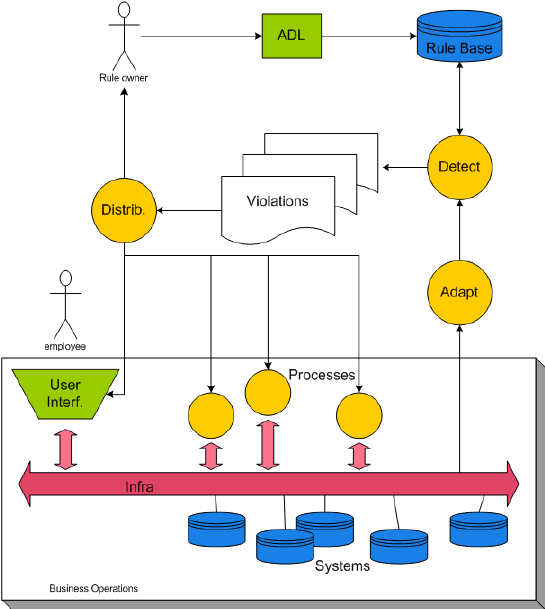
\includegraphics[width=7cm, height=6cm]{Principle-of-rule-based-process-management.png}
\caption{rule-based-proces}
\label{fig:rule-based-proces}
\end{wrapfigure}


The principle of rule-based \acrfull{bpm} as mentioned in \citepNonPub{joosten_joosten} is that any violation of a business rule may be used to trigger actions. 
This is described in the section \nameref{reactive_approach}.

Ampersand consists of concepts that in turn consist of atoms.
An atom is an implementation of the concept.
Inside the \acrshort{big} is a concept "beroep" with associated atoms like "arts, tandarts, etc".
The concepts are given a name, and the name must be recognized by the business.
This also applies to the definition and purpose of the concepts.
These attributes are not mandatory, but when one wants to generate a functional design, these descriptions of the attributes are very useful.
\begin{lstlisting}[language=Octave] 
CONCEPT Beroep "Beroep van een persoon zoals bedoeld in de wet" 
PURPOSE CONCEPT Beroep 
{+Beroep dat uitgeoefend wordt+}
POPULATION Beroep CONTAINS [
    "arts",
    "tandarts",
    "apotheker",
    "gezondheidszorgpsycholoog",
    "psychotherapeut",
    "fysiotherapeut",
    "verloskundige",
    "verpleegkundige",
    "physician assistant",
    "orthopedagoog-generalist"
]
\end{lstlisting}

Concepts can have relationships with each other.
If the data of the concepts is true and the rules yield consistent data then the relationships between real data are facts.
These facts together form one truth.
Not all concepts are directly related.
Within the domain of the \acrshort{big} we could distinguish the concept of "registratie" and the concept of "beroep".
This name is also referred to within ~\citeNonPub{van_wet_2018} in article 3 of \acrshort{big}.
Even the name of the relationship is mentioned in this article, which the legislator calls a "beroepsbeoefenaar".
The law requires that data of the "registratie" be recorded, indicating the corresponding profession (beroep).
In Ampersand, this is modelled as follows.
On the one hand, the "beroep" and also the concept "registratie".
\begin{lstlisting}[language=Octave] 
    CONCEPT Registratie "De registratie van een persoon binnen het register" 
    PURPOSE CONCEPT Registratie 
    {+Vastlegging in het register geeft toegang tot uitoefenen taak binnen de gezondheidszorg+}
\end{lstlisting}
Between the "registratie" and the $persoon$ exists the relationship "beroepsbeoefenaar".
\begin{lstlisting}[language=Octave] 
RELATION beroepsbeoefenaar [Persoon*Registratie] 
MEANING "geregistreerd persoon"
POPULATION beroepsbeoefenaar CONTAINS 
[
  ("Piet",1);
  ("Susan",2);
  ("Gerard",3);
  ("John",4)
]\end{lstlisting}
Also adding the concepts of $persoon$ and $handeling$.
Persons may perform the medical actions, but only when they are qualified.
\begin{lstlisting}[language=Octave] 
    CONCEPT Persoon "Persoon die werkzaam wilt zijn binnen de zorg"
    PURPOSE CONCEPT Persoon 
    {+Vastleggen van de identiteit van de persoon+}
\end{lstlisting}
\begin{lstlisting}[language=Octave] 
    CONCEPT Handeling "Acties die uitgevoerd worden" 
    PURPOSE CONCEPT Handeling 
    {+Vastleggen van de mogelijke handelingen die uitgevoerd kunnen worden binnen de zorg+}
\end{lstlisting}
These concepts can lead us to the following scheme.
\begin{figure}[H] 
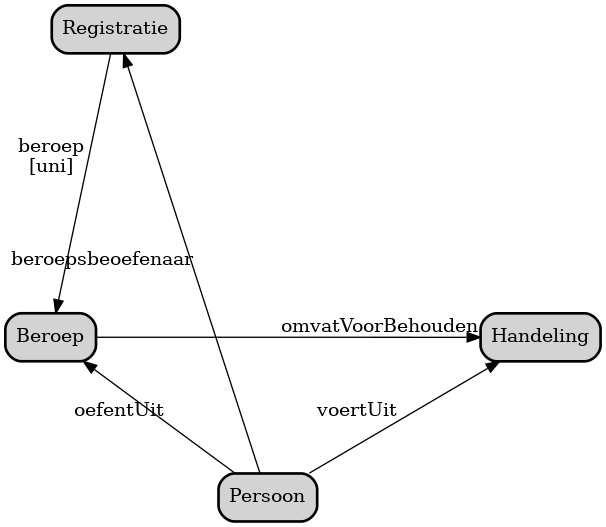
\includegraphics[scale=0.4]{CDConceptBeroep.png}
\centering
\caption{relations}
\label{fig:relations}
\end{figure}
The multiplicity must also be determined for each relation.
\begin{table}[h!]
    \begin{tabular}{||l | l||} 
     \hline
    function & The corresponding control question for the above relation $voerUit$ is\\
    \hline\hline
        Univalent & For each $Persoon$ there is at most 1 $Handeling$\\ %elke P max 1 H
        Total & For each $Persoon$ there is at least 1 $Handeling$ \\ %elke P minimaal 1 H
        Injective & For each $Handeling$ there is only 1 $Persoon$\\ %elke H max 1 P 
        Surjection & For each $Handeling$ there is at least 1 $Persoon$\\ %elke H minimaal 1 P
    \end{tabular}
    \caption{multiplicity}
    \label{tab:multiplicity}
\end{table}

By modelling using the Ampersand method, the question can be answered whether Ampersand provides more insight into the relationships.
As part of the research question, Ampersand can help you gain insight into the relationships.
Although you have to recognize and define these yourself, Ampersand will be helpful in generating functional design and prototype.
The generated prototype will validate the named constraints.
This will prevent registrations that do not meet the constraints.
These constraints are laid down in rules within Ampersand.
For example, a rule can be drawn up that determines whether a person is allowed to perform a certain action.
In figure \ref{fig:relations} the relations are named.
It was previously established that there are 2-tuple relationships.
Here we use the following notation:"$\mathit{relation [Concept \times Concept]}$".
\begin{center}
$\mathit{voertUit [Persoon \times Handeling]}$ ; 
 $\mathit{omvatVoorBehouden [Beroep \times Handeling]~\smallsmile}$
\newline $\subseteq$
\newline $\mathit{beroepsbeoefenaar [persoon \times registratie]}$ ;
$\mathit{beroep [registratie \times beroep]}$
\end{center}
The compared sets are
\newline $\mathit{[Persoon \times Beroep]}$
\newline The rule then will determine if the previous equation is true.
\newline If this is the case, then the rule is validated, otherwise the violation message occurs.
\begin{lstlisting}
    RULE HandelingDoorPersoon: voertUit; omvatVoorBehouden[Beroep*Handeling]~ |- beroepsbeoefenaar; beroep
    MEANING "Een persoon mag handelingen uitvoeren wanneer hij een bepaald beroep uitoefend"
    MESSAGE "Geen toegestane handeling."
    VIOLATION (TXT "Persoon ", SRC I, TXT " voert de handeling uit ", TGT I, TXT " die niet tot zijn beroep behoren ", SRC I[Persoon];oefentUit)
\end{lstlisting}


\subsection{Reactive approach} \label{reactive_approach}

The start of the reactive approach started with the reactive manifesto~\citepNonPub{reactive_manifesto}.
This defines the aspects that a reactive system should meet.
This includes Responsive, Resilient, Elastic and Message Driven.
These are systems that are flexible, loosely coupled and scalable and that makes them easier to develop and maintain.
Reactive Systems are made highly responsive and provide interactive feedback.
\begin{figure}[H] 
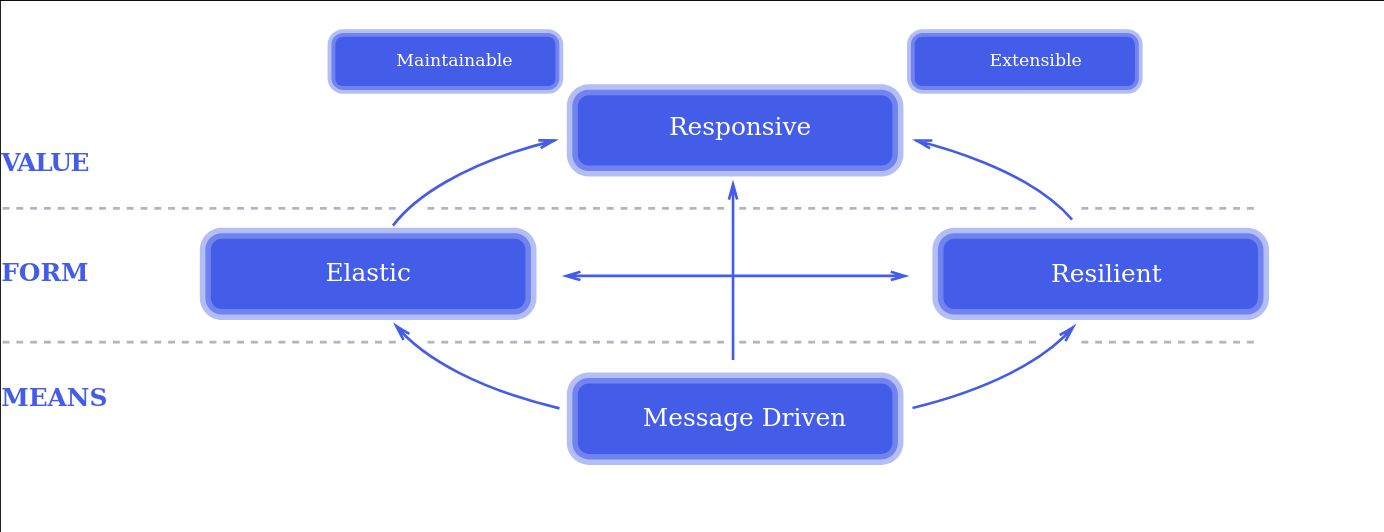
\includegraphics[scale=0.3]{reactive_manifesto.png}
\centering
\caption{reactive manifesto}
\label{fig:reactive manifesto}
\end{figure}


Ampersand is a form of Functional Reactive Programming (FRP)~\citep{elliott_functional_1997}.
The basic of reactive programming is the fact that it involves asynchronous communication.
This means that, as the \citeNonPub{reactive_manifesto} prescribes, use is made of message driven systems, but Ampersand is more than a message-driven system.
It is actually an event-driven system.
The glossary of the \citeNonPub{reactive_manifesto} indicates the difference between message driven systems and event driven systems.
An event-driven system targets event-bus while a message-driven system targets recipients~\citep{bainomugisha_survey_2013}.
The essence is that the order of the flow cannot be determined in advance.
The system will respond to events caused by constraints, Ampersand determines a dynamic flow~\citep{joosten_relation_2018}.




\subsubsection{Law analysis} \label{law_analysis}
The tax authorities have developed a method that is intended to analyse tax laws and other laws.
This is performed in these 6 steps:
\begin{enumerate}
    \item Determining the work area.
    \item Making the structure visible in legislation.
    \item Defining the meaning of legislation.
    \item Validate the analysis results.
    \item Identify missing execution policy.
    \item Setting up the knowledge model.
\end{enumerate}
Emphasis is placed on the cooperation between the implementer, ICT and policy.
By going through the method step by step, one arrives at a shared language.
This shared language includes the definition of concepts by the collaborating parties.
An important part of the approach is dividing the law into small pieces and always refer to these pieces of law in the implementation.
As a result, the method meets the requirement of the justification of government decisions.
The decisions are traceable, explainable, and it is possible to account for them.
What is not clear from the webinar~\citeNonPub{belastingdienst_webinar_2021} is how these steps were converted into an implementation.
The book~\citeNonPub{ausems_wetsanalyse_2021} indicates that the legal analysis method does not contain a development tool, but that the Tax and Customs Administration has developed an instrument based on the legal model, which is not freely available.

\subsection{Design method} \label{design_method}
The method used in this study is the Ampersand method.
The Ampersand method is based on relational algebra.
Ampersand makes it possible to make a conceptual analysis of problems. The data model created thereby makes it possible to accelerate implementation.


\subsubsection{Relation Algebra} \label{relation_algebra}
The field of the relation algebra, founded by De Morgan, focuses on operations with sets.
The signature item of relational algebra is the relationship, as the name implies.
This relationship has several properties, namely the attributes.
The attributes in the example of \acrshort{big} would be the surname, first names, gender, date of birth, nationality and address of the person concerned and the number and time of registration~\footnote{\acrlong{big} article 3, paragraph 2}.
In addition, the relationship consists of tuples.
Since the relationship is always between two objects, this is called 2-tuples.
The tuples contain the attributes of the relation.

Basically the operations on sets are the following:
\begin{itemize}
    \item Union, $R \cup S$ %vereniging
    \item Intersection, $R \cap S$ %doorsnede
    \item Difference, $R - S$ or $S - R$ %verschil
\end{itemize}
A distinction must be made between relation algebra and relational algebra.
Ampersand uses relation algebra, so is tuple related and the relational algebra is the foundation of e.g. relational databases.
This includes projections, selections and joins.
The latter are therefore not part of relation algebra.


\subsubsection{Ampersand} \label{ampersand}
Ampersand is based on relation algebra and focuses on business rules~\citepNonPub{wedemeijer_l_joosten_smm_michels_garkenbout_jlc_werkboek_ontwerpen_met_bedrijfsregelspdf_nodate}.
Ampersand supplies correct information systems.
In this case, Ampersand's goal is to provide a correct registry system.
Ampersand's other strengths are its support for conceptual analysis.
It is a platform for reactive programming and generates prototypes.
Ampersand describes the goals rather than the steps.

Business rules are there to pursue a common goal.
These rules are converted into an information system. 
The Ampersand method ensures that when a precise set of rules has been established, an information system can be generated. 
Ampersand focuses on business rules.
To learn how Ampersand works in real life, we design a registry in Ampersand that implements the \acrshort{big}~\citepNonPub{van_wet_2018} .

\begin{wrapfigure} {r}{0.52\textwidth} 
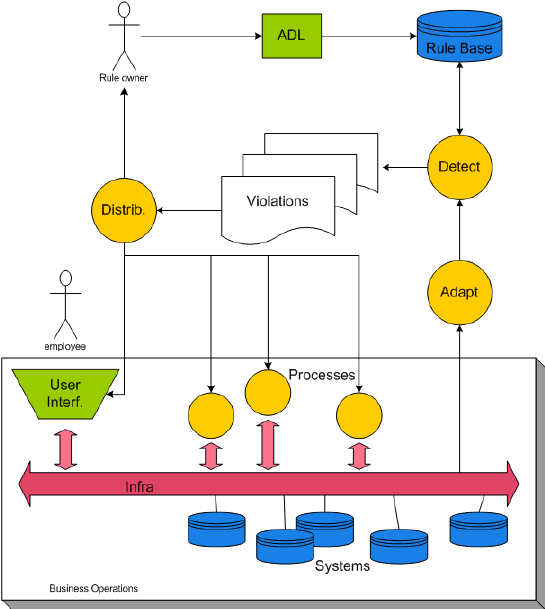
\includegraphics[width=7cm, height=6cm]{Principle-of-rule-based-process-management.png}
\caption{rule-based-proces}
\label{fig:rule-based-proces}
\end{wrapfigure}


The principle of rule-based \acrfull{bpm} as mentioned in \citepNonPub{joosten_joosten} is that any violation of a business rule may be used to trigger actions. 
This is described in the section \nameref{reactive_approach}.

Ampersand consists of concepts that in turn consist of atoms.
An atom is an implementation of the concept.
Inside the \acrshort{big} is a concept "beroep" with associated atoms like "arts, tandarts, etc".
The concepts are given a name, and the name must be recognized by the business.
This also applies to the definition and purpose of the concepts.
These attributes are not mandatory, but when one wants to generate a functional design, these descriptions of the attributes are very useful.
\begin{lstlisting}[language=Octave] 
CONCEPT Beroep "Beroep van een persoon zoals bedoeld in de wet" 
PURPOSE CONCEPT Beroep 
{+Beroep dat uitgeoefend wordt+}
POPULATION Beroep CONTAINS [
    "arts",
    "tandarts",
    "apotheker",
    "gezondheidszorgpsycholoog",
    "psychotherapeut",
    "fysiotherapeut",
    "verloskundige",
    "verpleegkundige",
    "physician assistant",
    "orthopedagoog-generalist"
]
\end{lstlisting}

Concepts can have relationships with each other.
If the data of the concepts is true and the rules yield consistent data then the relationships between real data are facts.
These facts together form one truth.
Not all concepts are directly related.
Within the domain of the \acrshort{big} we could distinguish the concept of "registratie" and the concept of "beroep".
This name is also referred to within ~\citeNonPub{van_wet_2018} in article 3 of \acrshort{big}.
Even the name of the relationship is mentioned in this article, which the legislator calls a "beroepsbeoefenaar".
The law requires that data of the "registratie" be recorded, indicating the corresponding profession (beroep).
In Ampersand, this is modelled as follows.
On the one hand, the "beroep" and also the concept "registratie".
\begin{lstlisting}[language=Octave] 
    CONCEPT Registratie "De registratie van een persoon binnen het register" 
    PURPOSE CONCEPT Registratie 
    {+Vastlegging in het register geeft toegang tot uitoefenen taak binnen de gezondheidszorg+}
\end{lstlisting}
Between the "registratie" and the $persoon$ exists the relationship "beroepsbeoefenaar".
\begin{lstlisting}[language=Octave] 
RELATION beroepsbeoefenaar [Persoon*Registratie] 
MEANING "geregistreerd persoon"
POPULATION beroepsbeoefenaar CONTAINS 
[
  ("Piet",1);
  ("Susan",2);
  ("Gerard",3);
  ("John",4)
]\end{lstlisting}
Also adding the concepts of $persoon$ and $handeling$.
Persons may perform the medical actions, but only when they are qualified.
\begin{lstlisting}[language=Octave] 
    CONCEPT Persoon "Persoon die werkzaam wilt zijn binnen de zorg"
    PURPOSE CONCEPT Persoon 
    {+Vastleggen van de identiteit van de persoon+}
\end{lstlisting}
\begin{lstlisting}[language=Octave] 
    CONCEPT Handeling "Acties die uitgevoerd worden" 
    PURPOSE CONCEPT Handeling 
    {+Vastleggen van de mogelijke handelingen die uitgevoerd kunnen worden binnen de zorg+}
\end{lstlisting}
These concepts can lead us to the following scheme.
\begin{figure}[H] 
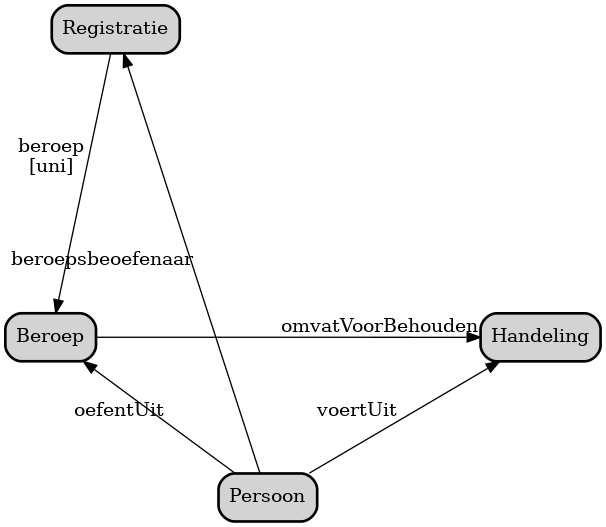
\includegraphics[scale=0.4]{CDConceptBeroep.png}
\centering
\caption{relations}
\label{fig:relations}
\end{figure}
The multiplicity must also be determined for each relation.
\begin{table}[h!]
    \begin{tabular}{||l | l||} 
     \hline
    function & The corresponding control question for the above relation $voerUit$ is\\
    \hline\hline
        Univalent & For each $Persoon$ there is at most 1 $Handeling$\\ %elke P max 1 H
        Total & For each $Persoon$ there is at least 1 $Handeling$ \\ %elke P minimaal 1 H
        Injective & For each $Handeling$ there is only 1 $Persoon$\\ %elke H max 1 P 
        Surjection & For each $Handeling$ there is at least 1 $Persoon$\\ %elke H minimaal 1 P
    \end{tabular}
    \caption{multiplicity}
    \label{tab:multiplicity}
\end{table}

By modelling using the Ampersand method, the question can be answered whether Ampersand provides more insight into the relationships.
As part of the research question, Ampersand can help you gain insight into the relationships.
Although you have to recognize and define these yourself, Ampersand will be helpful in generating functional design and prototype.
The generated prototype will validate the named constraints.
This will prevent registrations that do not meet the constraints.
These constraints are laid down in rules within Ampersand.
For example, a rule can be drawn up that determines whether a person is allowed to perform a certain action.
In figure \ref{fig:relations} the relations are named.
It was previously established that there are 2-tuple relationships.
Here we use the following notation:"$\mathit{relation [Concept \times Concept]}$".
\begin{center}
$\mathit{voertUit [Persoon \times Handeling]}$ ; 
 $\mathit{omvatVoorBehouden [Beroep \times Handeling]~\smallsmile}$
\newline $\subseteq$
\newline $\mathit{beroepsbeoefenaar [persoon \times registratie]}$ ;
$\mathit{beroep [registratie \times beroep]}$
\end{center}
The compared sets are
\newline $\mathit{[Persoon \times Beroep]}$
\newline The rule then will determine if the previous equation is true.
\newline If this is the case, then the rule is validated, otherwise the violation message occurs.
\begin{lstlisting}
    RULE HandelingDoorPersoon: voertUit; omvatVoorBehouden[Beroep*Handeling]~ |- beroepsbeoefenaar; beroep
    MEANING "Een persoon mag handelingen uitvoeren wanneer hij een bepaald beroep uitoefend"
    MESSAGE "Geen toegestane handeling."
    VIOLATION (TXT "Persoon ", SRC I, TXT " voert de handeling uit ", TGT I, TXT " die niet tot zijn beroep behoren ", SRC I[Persoon];oefentUit)
\end{lstlisting}


\subsection{Reactive approach} \label{reactive_approach}

The start of the reactive approach started with the reactive manifesto~\citepNonPub{reactive_manifesto}.
This defines the aspects that a reactive system should meet.
This includes Responsive, Resilient, Elastic and Message Driven.
These are systems that are flexible, loosely coupled and scalable and that makes them easier to develop and maintain.
Reactive Systems are made highly responsive and provide interactive feedback.
\begin{figure}[H] 
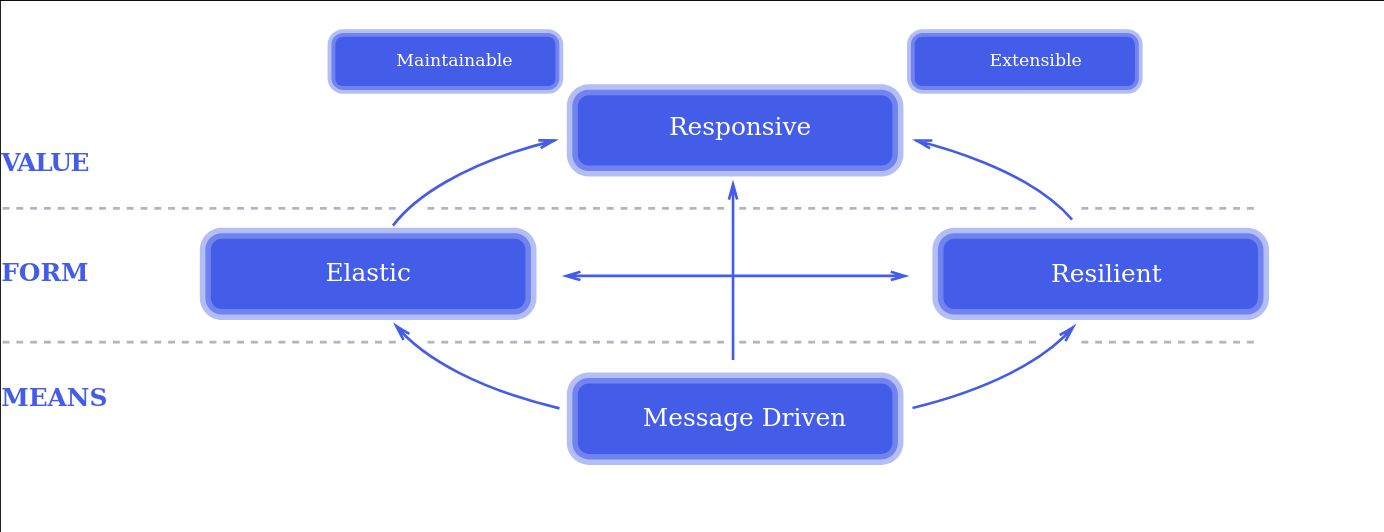
\includegraphics[scale=0.3]{reactive_manifesto.png}
\centering
\caption{reactive manifesto}
\label{fig:reactive manifesto}
\end{figure}


Ampersand is a form of Functional Reactive Programming (FRP)~\citep{elliott_functional_1997}.
The basic of reactive programming is the fact that it involves asynchronous communication.
This means that, as the \citeNonPub{reactive_manifesto} prescribes, use is made of message driven systems, but Ampersand is more than a message-driven system.
It is actually an event-driven system.
The glossary of the \citeNonPub{reactive_manifesto} indicates the difference between message driven systems and event driven systems.
An event-driven system targets event-bus while a message-driven system targets recipients~\citep{bainomugisha_survey_2013}.
The essence is that the order of the flow cannot be determined in advance.
The system will respond to events caused by constraints, Ampersand determines a dynamic flow~\citep{joosten_relation_2018}.




\subsubsection{Law analysis} \label{law_analysis}
The tax authorities have developed a method that is intended to analyse tax laws and other laws.
This is performed in these 6 steps:
\begin{enumerate}
    \item Determining the work area.
    \item Making the structure visible in legislation.
    \item Defining the meaning of legislation.
    \item Validate the analysis results.
    \item Identify missing execution policy.
    \item Setting up the knowledge model.
\end{enumerate}
Emphasis is placed on the cooperation between the implementer, ICT and policy.
By going through the method step by step, one arrives at a shared language.
This shared language includes the definition of concepts by the collaborating parties.
An important part of the approach is dividing the law into small pieces and always refer to these pieces of law in the implementation.
As a result, the method meets the requirement of the justification of government decisions.
The decisions are traceable, explainable, and it is possible to account for them.
What is not clear from the webinar~\citeNonPub{belastingdienst_webinar_2021} is how these steps were converted into an implementation.
The book~\citeNonPub{ausems_wetsanalyse_2021} indicates that the legal analysis method does not contain a development tool, but that the Tax and Customs Administration has developed an instrument based on the legal model, which is not freely available.
\subsection{Design method} \label{design_method}
The method used in this study is the Ampersand method.
The Ampersand method is based on relational algebra.
Ampersand makes it possible to make a conceptual analysis of problems. The data model created thereby makes it possible to accelerate implementation.


\subsubsection{Relation Algebra} \label{relation_algebra}
The field of the relation algebra, founded by De Morgan, focuses on operations with sets.
The signature item of relational algebra is the relationship, as the name implies.
This relationship has several properties, namely the attributes.
The attributes in the example of \acrshort{big} would be the surname, first names, gender, date of birth, nationality and address of the person concerned and the number and time of registration~\footnote{\acrlong{big} article 3, paragraph 2}.
In addition, the relationship consists of tuples.
Since the relationship is always between two objects, this is called 2-tuples.
The tuples contain the attributes of the relation.

Basically the operations on sets are the following:
\begin{itemize}
    \item Union, $R \cup S$ %vereniging
    \item Intersection, $R \cap S$ %doorsnede
    \item Difference, $R - S$ or $S - R$ %verschil
\end{itemize}
A distinction must be made between relation algebra and relational algebra.
Ampersand uses relation algebra, so is tuple related and the relational algebra is the foundation of e.g. relational databases.
This includes projections, selections and joins.
The latter are therefore not part of relation algebra.


\subsubsection{Ampersand} \label{ampersand}
Ampersand is based on relation algebra and focuses on business rules~\citepNonPub{wedemeijer_l_joosten_smm_michels_garkenbout_jlc_werkboek_ontwerpen_met_bedrijfsregelspdf_nodate}.
Ampersand supplies correct information systems.
In this case, Ampersand's goal is to provide a correct registry system.
Ampersand's other strengths are its support for conceptual analysis.
It is a platform for reactive programming and generates prototypes.
Ampersand describes the goals rather than the steps.

Business rules are there to pursue a common goal.
These rules are converted into an information system. 
The Ampersand method ensures that when a precise set of rules has been established, an information system can be generated. 
Ampersand focuses on business rules.
To learn how Ampersand works in real life, we design a registry in Ampersand that implements the \acrshort{big}~\citepNonPub{van_wet_2018} .

\begin{wrapfigure} {r}{0.52\textwidth} 
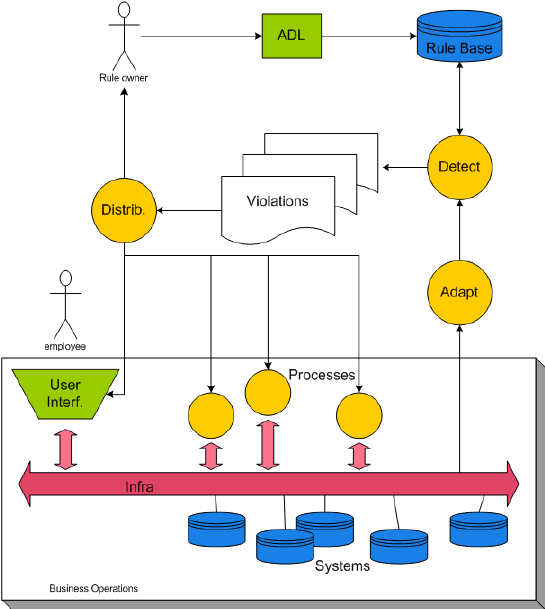
\includegraphics[width=7cm, height=6cm]{Principle-of-rule-based-process-management.png}
\caption{rule-based-proces}
\label{fig:rule-based-proces}
\end{wrapfigure}


The principle of rule-based \acrfull{bpm} as mentioned in \citepNonPub{joosten_joosten} is that any violation of a business rule may be used to trigger actions. 
This is described in the section \nameref{reactive_approach}.

Ampersand consists of concepts that in turn consist of atoms.
An atom is an implementation of the concept.
Inside the \acrshort{big} is a concept "beroep" with associated atoms like "arts, tandarts, etc".
The concepts are given a name, and the name must be recognized by the business.
This also applies to the definition and purpose of the concepts.
These attributes are not mandatory, but when one wants to generate a functional design, these descriptions of the attributes are very useful.
\begin{lstlisting}[language=Octave] 
CONCEPT Beroep "Beroep van een persoon zoals bedoeld in de wet" 
PURPOSE CONCEPT Beroep 
{+Beroep dat uitgeoefend wordt+}
POPULATION Beroep CONTAINS [
    "arts",
    "tandarts",
    "apotheker",
    "gezondheidszorgpsycholoog",
    "psychotherapeut",
    "fysiotherapeut",
    "verloskundige",
    "verpleegkundige",
    "physician assistant",
    "orthopedagoog-generalist"
]
\end{lstlisting}

Concepts can have relationships with each other.
If the data of the concepts is true and the rules yield consistent data then the relationships between real data are facts.
These facts together form one truth.
Not all concepts are directly related.
Within the domain of the \acrshort{big} we could distinguish the concept of "registratie" and the concept of "beroep".
This name is also referred to within ~\citeNonPub{van_wet_2018} in article 3 of \acrshort{big}.
Even the name of the relationship is mentioned in this article, which the legislator calls a "beroepsbeoefenaar".
The law requires that data of the "registratie" be recorded, indicating the corresponding profession (beroep).
In Ampersand, this is modelled as follows.
On the one hand, the "beroep" and also the concept "registratie".
\begin{lstlisting}[language=Octave] 
    CONCEPT Registratie "De registratie van een persoon binnen het register" 
    PURPOSE CONCEPT Registratie 
    {+Vastlegging in het register geeft toegang tot uitoefenen taak binnen de gezondheidszorg+}
\end{lstlisting}
Between the "registratie" and the $persoon$ exists the relationship "beroepsbeoefenaar".
\begin{lstlisting}[language=Octave] 
RELATION beroepsbeoefenaar [Persoon*Registratie] 
MEANING "geregistreerd persoon"
POPULATION beroepsbeoefenaar CONTAINS 
[
  ("Piet",1);
  ("Susan",2);
  ("Gerard",3);
  ("John",4)
]\end{lstlisting}
Also adding the concepts of $persoon$ and $handeling$.
Persons may perform the medical actions, but only when they are qualified.
\begin{lstlisting}[language=Octave] 
    CONCEPT Persoon "Persoon die werkzaam wilt zijn binnen de zorg"
    PURPOSE CONCEPT Persoon 
    {+Vastleggen van de identiteit van de persoon+}
\end{lstlisting}
\begin{lstlisting}[language=Octave] 
    CONCEPT Handeling "Acties die uitgevoerd worden" 
    PURPOSE CONCEPT Handeling 
    {+Vastleggen van de mogelijke handelingen die uitgevoerd kunnen worden binnen de zorg+}
\end{lstlisting}
These concepts can lead us to the following scheme.
\begin{figure}[H] 
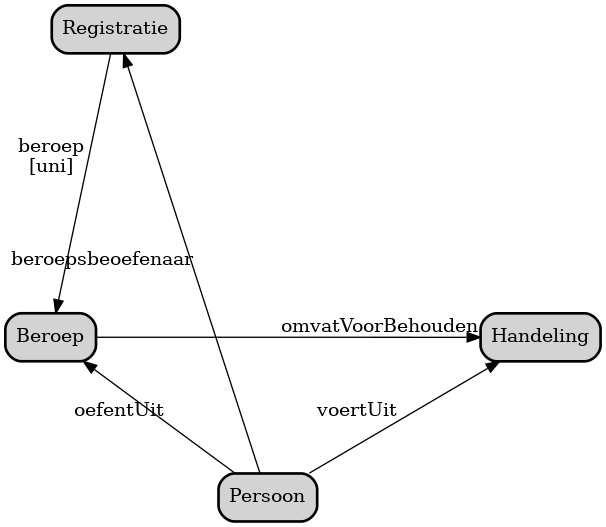
\includegraphics[scale=0.4]{CDConceptBeroep.png}
\centering
\caption{relations}
\label{fig:relations}
\end{figure}
The multiplicity must also be determined for each relation.
\begin{table}[h!]
    \begin{tabular}{||l | l||} 
     \hline
    function & The corresponding control question for the above relation $voerUit$ is\\
    \hline\hline
        Univalent & For each $Persoon$ there is at most 1 $Handeling$\\ %elke P max 1 H
        Total & For each $Persoon$ there is at least 1 $Handeling$ \\ %elke P minimaal 1 H
        Injective & For each $Handeling$ there is only 1 $Persoon$\\ %elke H max 1 P 
        Surjection & For each $Handeling$ there is at least 1 $Persoon$\\ %elke H minimaal 1 P
    \end{tabular}
    \caption{multiplicity}
    \label{tab:multiplicity}
\end{table}

By modelling using the Ampersand method, the question can be answered whether Ampersand provides more insight into the relationships.
As part of the research question, Ampersand can help you gain insight into the relationships.
Although you have to recognize and define these yourself, Ampersand will be helpful in generating functional design and prototype.
The generated prototype will validate the named constraints.
This will prevent registrations that do not meet the constraints.
These constraints are laid down in rules within Ampersand.
For example, a rule can be drawn up that determines whether a person is allowed to perform a certain action.
In figure \ref{fig:relations} the relations are named.
It was previously established that there are 2-tuple relationships.
Here we use the following notation:"$\mathit{relation [Concept \times Concept]}$".
\begin{center}
$\mathit{voertUit [Persoon \times Handeling]}$ ; 
 $\mathit{omvatVoorBehouden [Beroep \times Handeling]~\smallsmile}$
\newline $\subseteq$
\newline $\mathit{beroepsbeoefenaar [persoon \times registratie]}$ ;
$\mathit{beroep [registratie \times beroep]}$
\end{center}
The compared sets are
\newline $\mathit{[Persoon \times Beroep]}$
\newline The rule then will determine if the previous equation is true.
\newline If this is the case, then the rule is validated, otherwise the violation message occurs.
\begin{lstlisting}
    RULE HandelingDoorPersoon: voertUit; omvatVoorBehouden[Beroep*Handeling]~ |- beroepsbeoefenaar; beroep
    MEANING "Een persoon mag handelingen uitvoeren wanneer hij een bepaald beroep uitoefend"
    MESSAGE "Geen toegestane handeling."
    VIOLATION (TXT "Persoon ", SRC I, TXT " voert de handeling uit ", TGT I, TXT " die niet tot zijn beroep behoren ", SRC I[Persoon];oefentUit)
\end{lstlisting}


\subsection{Reactive approach} \label{reactive_approach}

The start of the reactive approach started with the reactive manifesto~\citepNonPub{reactive_manifesto}.
This defines the aspects that a reactive system should meet.
This includes Responsive, Resilient, Elastic and Message Driven.
These are systems that are flexible, loosely coupled and scalable and that makes them easier to develop and maintain.
Reactive Systems are made highly responsive and provide interactive feedback.
\begin{figure}[H] 
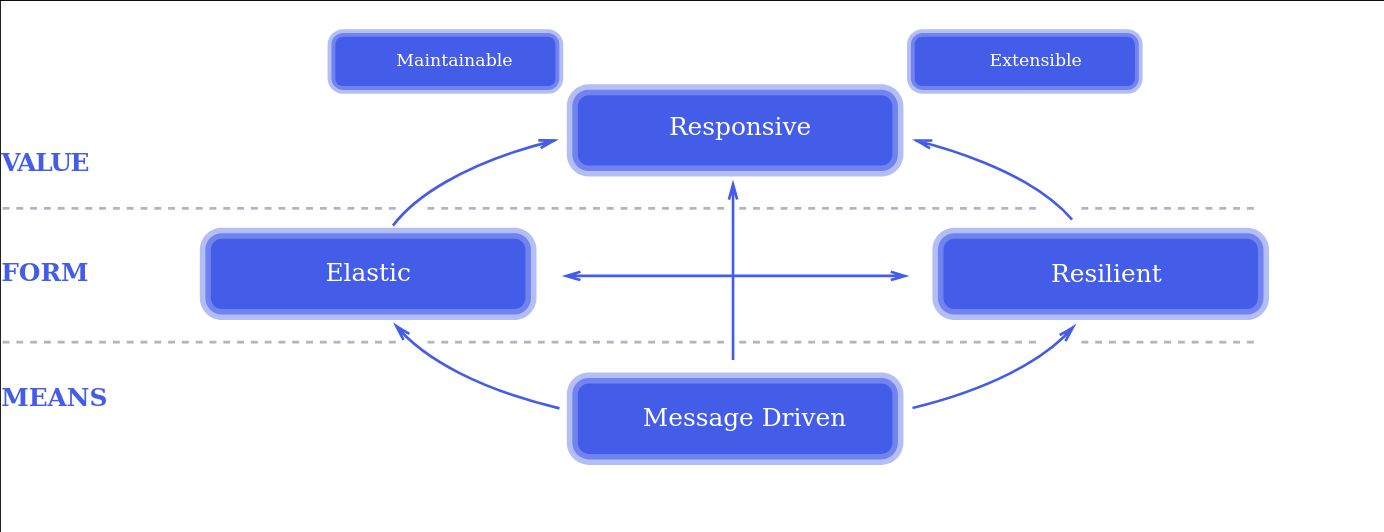
\includegraphics[scale=0.3]{reactive_manifesto.png}
\centering
\caption{reactive manifesto}
\label{fig:reactive manifesto}
\end{figure}


Ampersand is a form of Functional Reactive Programming (FRP)~\citep{elliott_functional_1997}.
The basic of reactive programming is the fact that it involves asynchronous communication.
This means that, as the \citeNonPub{reactive_manifesto} prescribes, use is made of message driven systems, but Ampersand is more than a message-driven system.
It is actually an event-driven system.
The glossary of the \citeNonPub{reactive_manifesto} indicates the difference between message driven systems and event driven systems.
An event-driven system targets event-bus while a message-driven system targets recipients~\citep{bainomugisha_survey_2013}.
The essence is that the order of the flow cannot be determined in advance.
The system will respond to events caused by constraints, Ampersand determines a dynamic flow~\citep{joosten_relation_2018}.




\subsubsection{Law analysis} \label{law_analysis}
The tax authorities have developed a method that is intended to analyse tax laws and other laws.
This is performed in these 6 steps:
\begin{enumerate}
    \item Determining the work area.
    \item Making the structure visible in legislation.
    \item Defining the meaning of legislation.
    \item Validate the analysis results.
    \item Identify missing execution policy.
    \item Setting up the knowledge model.
\end{enumerate}
Emphasis is placed on the cooperation between the implementer, ICT and policy.
By going through the method step by step, one arrives at a shared language.
This shared language includes the definition of concepts by the collaborating parties.
An important part of the approach is dividing the law into small pieces and always refer to these pieces of law in the implementation.
As a result, the method meets the requirement of the justification of government decisions.
The decisions are traceable, explainable, and it is possible to account for them.
What is not clear from the webinar~\citeNonPub{belastingdienst_webinar_2021} is how these steps were converted into an implementation.
The book~\citeNonPub{ausems_wetsanalyse_2021} indicates that the legal analysis method does not contain a development tool, but that the Tax and Customs Administration has developed an instrument based on the legal model, which is not freely available.
\subsection{Design method} \label{design_method}
The method used in this study is the Ampersand method.
The Ampersand method is based on relational algebra.
Ampersand makes it possible to make a conceptual analysis of problems. The data model created thereby makes it possible to accelerate implementation.


\subsubsection{Relation Algebra} \label{relation_algebra}
The field of the relation algebra, founded by De Morgan, focuses on operations with sets.
The signature item of relational algebra is the relationship, as the name implies.
This relationship has several properties, namely the attributes.
The attributes in the example of \acrshort{big} would be the surname, first names, gender, date of birth, nationality and address of the person concerned and the number and time of registration~\footnote{\acrlong{big} article 3, paragraph 2}.
In addition, the relationship consists of tuples.
Since the relationship is always between two objects, this is called 2-tuples.
The tuples contain the attributes of the relation.

Basically the operations on sets are the following:
\begin{itemize}
    \item Union, $R \cup S$ %vereniging
    \item Intersection, $R \cap S$ %doorsnede
    \item Difference, $R - S$ or $S - R$ %verschil
\end{itemize}
A distinction must be made between relation algebra and relational algebra.
Ampersand uses relation algebra, so is tuple related and the relational algebra is the foundation of e.g. relational databases.
This includes projections, selections and joins.
The latter are therefore not part of relation algebra.


\subsubsection{Ampersand} \label{ampersand}
Ampersand is based on relation algebra and focuses on business rules~\citepNonPub{wedemeijer_l_joosten_smm_michels_garkenbout_jlc_werkboek_ontwerpen_met_bedrijfsregelspdf_nodate}.
Ampersand supplies correct information systems.
In this case, Ampersand's goal is to provide a correct registry system.
Ampersand's other strengths are its support for conceptual analysis.
It is a platform for reactive programming and generates prototypes.
Ampersand describes the goals rather than the steps.

Business rules are there to pursue a common goal.
These rules are converted into an information system. 
The Ampersand method ensures that when a precise set of rules has been established, an information system can be generated. 
Ampersand focuses on business rules.
To learn how Ampersand works in real life, we design a registry in Ampersand that implements the \acrshort{big}~\citepNonPub{van_wet_2018} .

\begin{wrapfigure} {r}{0.52\textwidth} 
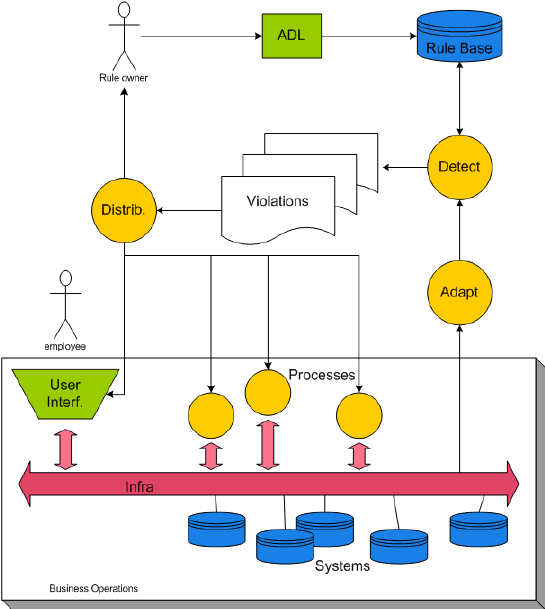
\includegraphics[width=7cm, height=6cm]{Principle-of-rule-based-process-management.png}
\caption{rule-based-proces}
\label{fig:rule-based-proces}
\end{wrapfigure}


The principle of rule-based \acrfull{bpm} as mentioned in \citepNonPub{joosten_joosten} is that any violation of a business rule may be used to trigger actions. 
This is described in the section \nameref{reactive_approach}.

Ampersand consists of concepts that in turn consist of atoms.
An atom is an implementation of the concept.
Inside the \acrshort{big} is a concept "beroep" with associated atoms like "arts, tandarts, etc".
The concepts are given a name, and the name must be recognized by the business.
This also applies to the definition and purpose of the concepts.
These attributes are not mandatory, but when one wants to generate a functional design, these descriptions of the attributes are very useful.
\begin{lstlisting}[language=Octave] 
CONCEPT Beroep "Beroep van een persoon zoals bedoeld in de wet" 
PURPOSE CONCEPT Beroep 
{+Beroep dat uitgeoefend wordt+}
POPULATION Beroep CONTAINS [
    "arts",
    "tandarts",
    "apotheker",
    "gezondheidszorgpsycholoog",
    "psychotherapeut",
    "fysiotherapeut",
    "verloskundige",
    "verpleegkundige",
    "physician assistant",
    "orthopedagoog-generalist"
]
\end{lstlisting}

Concepts can have relationships with each other.
If the data of the concepts is true and the rules yield consistent data then the relationships between real data are facts.
These facts together form one truth.
Not all concepts are directly related.
Within the domain of the \acrshort{big} we could distinguish the concept of "registratie" and the concept of "beroep".
This name is also referred to within ~\citeNonPub{van_wet_2018} in article 3 of \acrshort{big}.
Even the name of the relationship is mentioned in this article, which the legislator calls a "beroepsbeoefenaar".
The law requires that data of the "registratie" be recorded, indicating the corresponding profession (beroep).
In Ampersand, this is modelled as follows.
On the one hand, the "beroep" and also the concept "registratie".
\begin{lstlisting}[language=Octave] 
    CONCEPT Registratie "De registratie van een persoon binnen het register" 
    PURPOSE CONCEPT Registratie 
    {+Vastlegging in het register geeft toegang tot uitoefenen taak binnen de gezondheidszorg+}
\end{lstlisting}
Between the "registratie" and the $persoon$ exists the relationship "beroepsbeoefenaar".
\begin{lstlisting}[language=Octave] 
RELATION beroepsbeoefenaar [Persoon*Registratie] 
MEANING "geregistreerd persoon"
POPULATION beroepsbeoefenaar CONTAINS 
[
  ("Piet",1);
  ("Susan",2);
  ("Gerard",3);
  ("John",4)
]\end{lstlisting}
Also adding the concepts of $persoon$ and $handeling$.
Persons may perform the medical actions, but only when they are qualified.
\begin{lstlisting}[language=Octave] 
    CONCEPT Persoon "Persoon die werkzaam wilt zijn binnen de zorg"
    PURPOSE CONCEPT Persoon 
    {+Vastleggen van de identiteit van de persoon+}
\end{lstlisting}
\begin{lstlisting}[language=Octave] 
    CONCEPT Handeling "Acties die uitgevoerd worden" 
    PURPOSE CONCEPT Handeling 
    {+Vastleggen van de mogelijke handelingen die uitgevoerd kunnen worden binnen de zorg+}
\end{lstlisting}
These concepts can lead us to the following scheme.
\begin{figure}[H] 
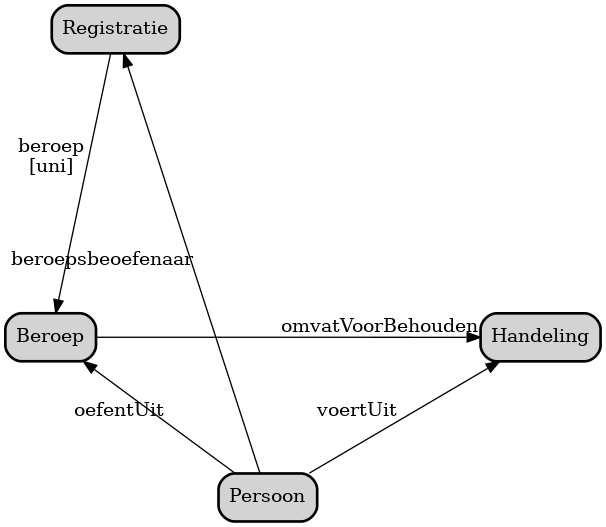
\includegraphics[scale=0.4]{CDConceptBeroep.png}
\centering
\caption{relations}
\label{fig:relations}
\end{figure}
The multiplicity must also be determined for each relation.
\begin{table}[h!]
    \begin{tabular}{||l | l||} 
     \hline
    function & The corresponding control question for the above relation $voerUit$ is\\
    \hline\hline
        Univalent & For each $Persoon$ there is at most 1 $Handeling$\\ %elke P max 1 H
        Total & For each $Persoon$ there is at least 1 $Handeling$ \\ %elke P minimaal 1 H
        Injective & For each $Handeling$ there is only 1 $Persoon$\\ %elke H max 1 P 
        Surjection & For each $Handeling$ there is at least 1 $Persoon$\\ %elke H minimaal 1 P
    \end{tabular}
    \caption{multiplicity}
    \label{tab:multiplicity}
\end{table}

By modelling using the Ampersand method, the question can be answered whether Ampersand provides more insight into the relationships.
As part of the research question, Ampersand can help you gain insight into the relationships.
Although you have to recognize and define these yourself, Ampersand will be helpful in generating functional design and prototype.
The generated prototype will validate the named constraints.
This will prevent registrations that do not meet the constraints.
These constraints are laid down in rules within Ampersand.
For example, a rule can be drawn up that determines whether a person is allowed to perform a certain action.
In figure \ref{fig:relations} the relations are named.
It was previously established that there are 2-tuple relationships.
Here we use the following notation:"$\mathit{relation [Concept \times Concept]}$".
\begin{center}
$\mathit{voertUit [Persoon \times Handeling]}$ ; 
 $\mathit{omvatVoorBehouden [Beroep \times Handeling]~\smallsmile}$
\newline $\subseteq$
\newline $\mathit{beroepsbeoefenaar [persoon \times registratie]}$ ;
$\mathit{beroep [registratie \times beroep]}$
\end{center}
The compared sets are
\newline $\mathit{[Persoon \times Beroep]}$
\newline The rule then will determine if the previous equation is true.
\newline If this is the case, then the rule is validated, otherwise the violation message occurs.
\begin{lstlisting}
    RULE HandelingDoorPersoon: voertUit; omvatVoorBehouden[Beroep*Handeling]~ |- beroepsbeoefenaar; beroep
    MEANING "Een persoon mag handelingen uitvoeren wanneer hij een bepaald beroep uitoefend"
    MESSAGE "Geen toegestane handeling."
    VIOLATION (TXT "Persoon ", SRC I, TXT " voert de handeling uit ", TGT I, TXT " die niet tot zijn beroep behoren ", SRC I[Persoon];oefentUit)
\end{lstlisting}


\subsection{Reactive approach} \label{reactive_approach}

The start of the reactive approach started with the reactive manifesto~\citepNonPub{reactive_manifesto}.
This defines the aspects that a reactive system should meet.
This includes Responsive, Resilient, Elastic and Message Driven.
These are systems that are flexible, loosely coupled and scalable and that makes them easier to develop and maintain.
Reactive Systems are made highly responsive and provide interactive feedback.
\begin{figure}[H] 
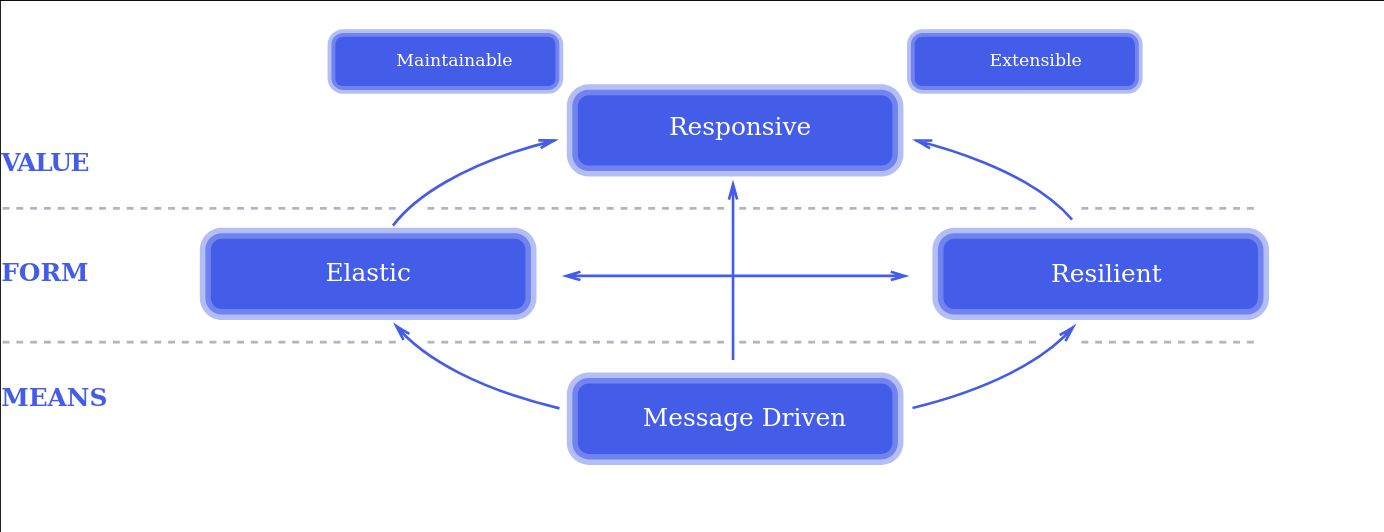
\includegraphics[scale=0.3]{reactive_manifesto.png}
\centering
\caption{reactive manifesto}
\label{fig:reactive manifesto}
\end{figure}


Ampersand is a form of Functional Reactive Programming (FRP)~\citep{elliott_functional_1997}.
The basic of reactive programming is the fact that it involves asynchronous communication.
This means that, as the \citeNonPub{reactive_manifesto} prescribes, use is made of message driven systems, but Ampersand is more than a message-driven system.
It is actually an event-driven system.
The glossary of the \citeNonPub{reactive_manifesto} indicates the difference between message driven systems and event driven systems.
An event-driven system targets event-bus while a message-driven system targets recipients~\citep{bainomugisha_survey_2013}.
The essence is that the order of the flow cannot be determined in advance.
The system will respond to events caused by constraints, Ampersand determines a dynamic flow~\citep{joosten_relation_2018}.




\subsubsection{Law analysis} \label{law_analysis}
The tax authorities have developed a method that is intended to analyse tax laws and other laws.
This is performed in these 6 steps:
\begin{enumerate}
    \item Determining the work area.
    \item Making the structure visible in legislation.
    \item Defining the meaning of legislation.
    \item Validate the analysis results.
    \item Identify missing execution policy.
    \item Setting up the knowledge model.
\end{enumerate}
Emphasis is placed on the cooperation between the implementer, ICT and policy.
By going through the method step by step, one arrives at a shared language.
This shared language includes the definition of concepts by the collaborating parties.
An important part of the approach is dividing the law into small pieces and always refer to these pieces of law in the implementation.
As a result, the method meets the requirement of the justification of government decisions.
The decisions are traceable, explainable, and it is possible to account for them.
What is not clear from the webinar~\citeNonPub{belastingdienst_webinar_2021} is how these steps were converted into an implementation.
The book~\citeNonPub{ausems_wetsanalyse_2021} indicates that the legal analysis method does not contain a development tool, but that the Tax and Customs Administration has developed an instrument based on the legal model, which is not freely available.

\subsection{Design method} \label{design_method}
The method used in this study is the Ampersand method.
The Ampersand method is based on relational algebra.
Ampersand makes it possible to make a conceptual analysis of problems. The data model created thereby makes it possible to accelerate implementation.


\subsubsection{Relation Algebra} \label{relation_algebra}
The field of the relation algebra, founded by De Morgan, focuses on operations with sets.
The signature item of relational algebra is the relationship, as the name implies.
This relationship has several properties, namely the attributes.
The attributes in the example of \acrshort{big} would be the surname, first names, gender, date of birth, nationality and address of the person concerned and the number and time of registration~\footnote{\acrlong{big} article 3, paragraph 2}.
In addition, the relationship consists of tuples.
Since the relationship is always between two objects, this is called 2-tuples.
The tuples contain the attributes of the relation.

Basically the operations on sets are the following:
\begin{itemize}
    \item Union, $R \cup S$ %vereniging
    \item Intersection, $R \cap S$ %doorsnede
    \item Difference, $R - S$ or $S - R$ %verschil
\end{itemize}
A distinction must be made between relation algebra and relational algebra.
Ampersand uses relation algebra, so is tuple related and the relational algebra is the foundation of e.g. relational databases.
This includes projections, selections and joins.
The latter are therefore not part of relation algebra.


\subsubsection{Ampersand} \label{ampersand}
Ampersand is based on relation algebra and focuses on business rules~\citepNonPub{wedemeijer_l_joosten_smm_michels_garkenbout_jlc_werkboek_ontwerpen_met_bedrijfsregelspdf_nodate}.
Ampersand supplies correct information systems.
In this case, Ampersand's goal is to provide a correct registry system.
Ampersand's other strengths are its support for conceptual analysis.
It is a platform for reactive programming and generates prototypes.
Ampersand describes the goals rather than the steps.

Business rules are there to pursue a common goal.
These rules are converted into an information system. 
The Ampersand method ensures that when a precise set of rules has been established, an information system can be generated. 
Ampersand focuses on business rules.
To learn how Ampersand works in real life, we design a registry in Ampersand that implements the \acrshort{big}~\citepNonPub{van_wet_2018} .

\begin{wrapfigure} {r}{0.52\textwidth} 
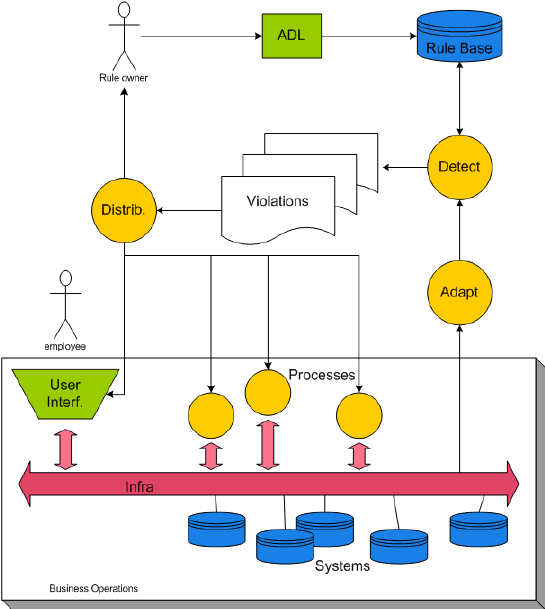
\includegraphics[width=7cm, height=6cm]{Principle-of-rule-based-process-management.png}
\caption{rule-based-proces}
\label{fig:rule-based-proces}
\end{wrapfigure}


The principle of rule-based \acrfull{bpm} as mentioned in \citepNonPub{joosten_joosten} is that any violation of a business rule may be used to trigger actions. 
This is described in the section \nameref{reactive_approach}.

Ampersand consists of concepts that in turn consist of atoms.
An atom is an implementation of the concept.
Inside the \acrshort{big} is a concept "beroep" with associated atoms like "arts, tandarts, etc".
The concepts are given a name, and the name must be recognized by the business.
This also applies to the definition and purpose of the concepts.
These attributes are not mandatory, but when one wants to generate a functional design, these descriptions of the attributes are very useful.
\begin{lstlisting}[language=Octave] 
CONCEPT Beroep "Beroep van een persoon zoals bedoeld in de wet" 
PURPOSE CONCEPT Beroep 
{+Beroep dat uitgeoefend wordt+}
POPULATION Beroep CONTAINS [
    "arts",
    "tandarts",
    "apotheker",
    "gezondheidszorgpsycholoog",
    "psychotherapeut",
    "fysiotherapeut",
    "verloskundige",
    "verpleegkundige",
    "physician assistant",
    "orthopedagoog-generalist"
]
\end{lstlisting}

Concepts can have relationships with each other.
If the data of the concepts is true and the rules yield consistent data then the relationships between real data are facts.
These facts together form one truth.
Not all concepts are directly related.
Within the domain of the \acrshort{big} we could distinguish the concept of "registratie" and the concept of "beroep".
This name is also referred to within ~\citeNonPub{van_wet_2018} in article 3 of \acrshort{big}.
Even the name of the relationship is mentioned in this article, which the legislator calls a "beroepsbeoefenaar".
The law requires that data of the "registratie" be recorded, indicating the corresponding profession (beroep).
In Ampersand, this is modelled as follows.
On the one hand, the "beroep" and also the concept "registratie".
\begin{lstlisting}[language=Octave] 
    CONCEPT Registratie "De registratie van een persoon binnen het register" 
    PURPOSE CONCEPT Registratie 
    {+Vastlegging in het register geeft toegang tot uitoefenen taak binnen de gezondheidszorg+}
\end{lstlisting}
Between the "registratie" and the $persoon$ exists the relationship "beroepsbeoefenaar".
\begin{lstlisting}[language=Octave] 
RELATION beroepsbeoefenaar [Persoon*Registratie] 
MEANING "geregistreerd persoon"
POPULATION beroepsbeoefenaar CONTAINS 
[
  ("Piet",1);
  ("Susan",2);
  ("Gerard",3);
  ("John",4)
]\end{lstlisting}
Also adding the concepts of $persoon$ and $handeling$.
Persons may perform the medical actions, but only when they are qualified.
\begin{lstlisting}[language=Octave] 
    CONCEPT Persoon "Persoon die werkzaam wilt zijn binnen de zorg"
    PURPOSE CONCEPT Persoon 
    {+Vastleggen van de identiteit van de persoon+}
\end{lstlisting}
\begin{lstlisting}[language=Octave] 
    CONCEPT Handeling "Acties die uitgevoerd worden" 
    PURPOSE CONCEPT Handeling 
    {+Vastleggen van de mogelijke handelingen die uitgevoerd kunnen worden binnen de zorg+}
\end{lstlisting}
These concepts can lead us to the following scheme.
\begin{figure}[H] 
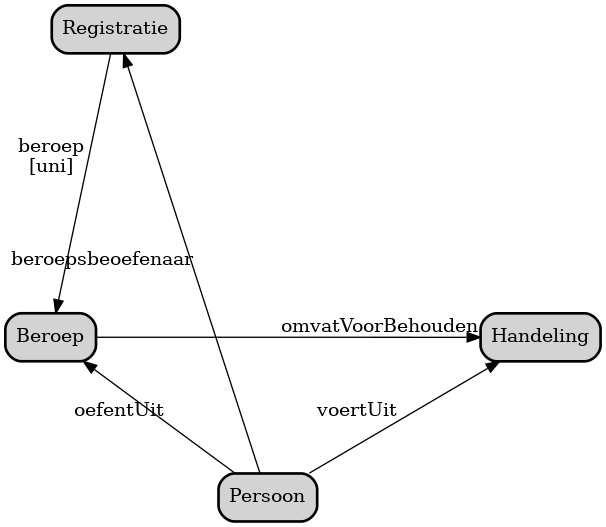
\includegraphics[scale=0.4]{CDConceptBeroep.png}
\centering
\caption{relations}
\label{fig:relations}
\end{figure}
The multiplicity must also be determined for each relation.
\begin{table}[h!]
    \begin{tabular}{||l | l||} 
     \hline
    function & The corresponding control question for the above relation $voerUit$ is\\
    \hline\hline
        Univalent & For each $Persoon$ there is at most 1 $Handeling$\\ %elke P max 1 H
        Total & For each $Persoon$ there is at least 1 $Handeling$ \\ %elke P minimaal 1 H
        Injective & For each $Handeling$ there is only 1 $Persoon$\\ %elke H max 1 P 
        Surjection & For each $Handeling$ there is at least 1 $Persoon$\\ %elke H minimaal 1 P
    \end{tabular}
    \caption{multiplicity}
    \label{tab:multiplicity}
\end{table}

By modelling using the Ampersand method, the question can be answered whether Ampersand provides more insight into the relationships.
As part of the research question, Ampersand can help you gain insight into the relationships.
Although you have to recognize and define these yourself, Ampersand will be helpful in generating functional design and prototype.
The generated prototype will validate the named constraints.
This will prevent registrations that do not meet the constraints.
These constraints are laid down in rules within Ampersand.
For example, a rule can be drawn up that determines whether a person is allowed to perform a certain action.
In figure \ref{fig:relations} the relations are named.
It was previously established that there are 2-tuple relationships.
Here we use the following notation:"$\mathit{relation [Concept \times Concept]}$".
\begin{center}
$\mathit{voertUit [Persoon \times Handeling]}$ ; 
 $\mathit{omvatVoorBehouden [Beroep \times Handeling]~\smallsmile}$
\newline $\subseteq$
\newline $\mathit{beroepsbeoefenaar [persoon \times registratie]}$ ;
$\mathit{beroep [registratie \times beroep]}$
\end{center}
The compared sets are
\newline $\mathit{[Persoon \times Beroep]}$
\newline The rule then will determine if the previous equation is true.
\newline If this is the case, then the rule is validated, otherwise the violation message occurs.
\begin{lstlisting}
    RULE HandelingDoorPersoon: voertUit; omvatVoorBehouden[Beroep*Handeling]~ |- beroepsbeoefenaar; beroep
    MEANING "Een persoon mag handelingen uitvoeren wanneer hij een bepaald beroep uitoefend"
    MESSAGE "Geen toegestane handeling."
    VIOLATION (TXT "Persoon ", SRC I, TXT " voert de handeling uit ", TGT I, TXT " die niet tot zijn beroep behoren ", SRC I[Persoon];oefentUit)
\end{lstlisting}


\subsection{Reactive approach} \label{reactive_approach}

The start of the reactive approach started with the reactive manifesto~\citepNonPub{reactive_manifesto}.
This defines the aspects that a reactive system should meet.
This includes Responsive, Resilient, Elastic and Message Driven.
These are systems that are flexible, loosely coupled and scalable and that makes them easier to develop and maintain.
Reactive Systems are made highly responsive and provide interactive feedback.
\begin{figure}[H] 
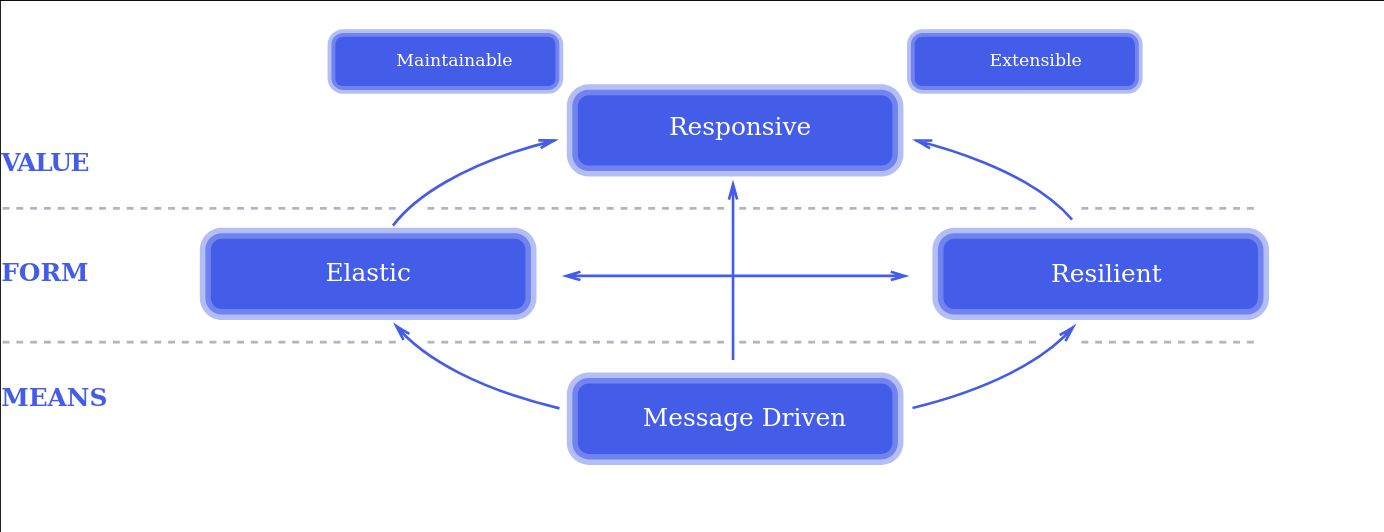
\includegraphics[scale=0.3]{reactive_manifesto.png}
\centering
\caption{reactive manifesto}
\label{fig:reactive manifesto}
\end{figure}


Ampersand is a form of Functional Reactive Programming (FRP)~\citep{elliott_functional_1997}.
The basic of reactive programming is the fact that it involves asynchronous communication.
This means that, as the \citeNonPub{reactive_manifesto} prescribes, use is made of message driven systems, but Ampersand is more than a message-driven system.
It is actually an event-driven system.
The glossary of the \citeNonPub{reactive_manifesto} indicates the difference between message driven systems and event driven systems.
An event-driven system targets event-bus while a message-driven system targets recipients~\citep{bainomugisha_survey_2013}.
The essence is that the order of the flow cannot be determined in advance.
The system will respond to events caused by constraints, Ampersand determines a dynamic flow~\citep{joosten_relation_2018}.




\subsubsection{Law analysis} \label{law_analysis}
The tax authorities have developed a method that is intended to analyse tax laws and other laws.
This is performed in these 6 steps:
\begin{enumerate}
    \item Determining the work area.
    \item Making the structure visible in legislation.
    \item Defining the meaning of legislation.
    \item Validate the analysis results.
    \item Identify missing execution policy.
    \item Setting up the knowledge model.
\end{enumerate}
Emphasis is placed on the cooperation between the implementer, ICT and policy.
By going through the method step by step, one arrives at a shared language.
This shared language includes the definition of concepts by the collaborating parties.
An important part of the approach is dividing the law into small pieces and always refer to these pieces of law in the implementation.
As a result, the method meets the requirement of the justification of government decisions.
The decisions are traceable, explainable, and it is possible to account for them.
What is not clear from the webinar~\citeNonPub{belastingdienst_webinar_2021} is how these steps were converted into an implementation.
The book~\citeNonPub{ausems_wetsanalyse_2021} indicates that the legal analysis method does not contain a development tool, but that the Tax and Customs Administration has developed an instrument based on the legal model, which is not freely available.
\subsection{Design method} \label{design_method}
The method used in this study is the Ampersand method.
The Ampersand method is based on relational algebra.
Ampersand makes it possible to make a conceptual analysis of problems. The data model created thereby makes it possible to accelerate implementation.


\subsubsection{Relation Algebra} \label{relation_algebra}
The field of the relation algebra, founded by De Morgan, focuses on operations with sets.
The signature item of relational algebra is the relationship, as the name implies.
This relationship has several properties, namely the attributes.
The attributes in the example of \acrshort{big} would be the surname, first names, gender, date of birth, nationality and address of the person concerned and the number and time of registration~\footnote{\acrlong{big} article 3, paragraph 2}.
In addition, the relationship consists of tuples.
Since the relationship is always between two objects, this is called 2-tuples.
The tuples contain the attributes of the relation.

Basically the operations on sets are the following:
\begin{itemize}
    \item Union, $R \cup S$ %vereniging
    \item Intersection, $R \cap S$ %doorsnede
    \item Difference, $R - S$ or $S - R$ %verschil
\end{itemize}
A distinction must be made between relation algebra and relational algebra.
Ampersand uses relation algebra, so is tuple related and the relational algebra is the foundation of e.g. relational databases.
This includes projections, selections and joins.
The latter are therefore not part of relation algebra.


\subsubsection{Ampersand} \label{ampersand}
Ampersand is based on relation algebra and focuses on business rules~\citepNonPub{wedemeijer_l_joosten_smm_michels_garkenbout_jlc_werkboek_ontwerpen_met_bedrijfsregelspdf_nodate}.
Ampersand supplies correct information systems.
In this case, Ampersand's goal is to provide a correct registry system.
Ampersand's other strengths are its support for conceptual analysis.
It is a platform for reactive programming and generates prototypes.
Ampersand describes the goals rather than the steps.

Business rules are there to pursue a common goal.
These rules are converted into an information system. 
The Ampersand method ensures that when a precise set of rules has been established, an information system can be generated. 
Ampersand focuses on business rules.
To learn how Ampersand works in real life, we design a registry in Ampersand that implements the \acrshort{big}~\citepNonPub{van_wet_2018} .

\begin{wrapfigure} {r}{0.52\textwidth} 
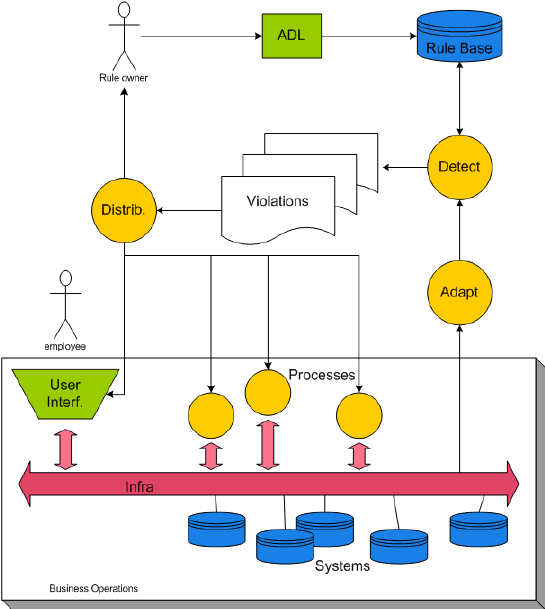
\includegraphics[width=7cm, height=6cm]{Principle-of-rule-based-process-management.png}
\caption{rule-based-proces}
\label{fig:rule-based-proces}
\end{wrapfigure}


The principle of rule-based \acrfull{bpm} as mentioned in \citepNonPub{joosten_joosten} is that any violation of a business rule may be used to trigger actions. 
This is described in the section \nameref{reactive_approach}.

Ampersand consists of concepts that in turn consist of atoms.
An atom is an implementation of the concept.
Inside the \acrshort{big} is a concept "beroep" with associated atoms like "arts, tandarts, etc".
The concepts are given a name, and the name must be recognized by the business.
This also applies to the definition and purpose of the concepts.
These attributes are not mandatory, but when one wants to generate a functional design, these descriptions of the attributes are very useful.
\begin{lstlisting}[language=Octave] 
CONCEPT Beroep "Beroep van een persoon zoals bedoeld in de wet" 
PURPOSE CONCEPT Beroep 
{+Beroep dat uitgeoefend wordt+}
POPULATION Beroep CONTAINS [
    "arts",
    "tandarts",
    "apotheker",
    "gezondheidszorgpsycholoog",
    "psychotherapeut",
    "fysiotherapeut",
    "verloskundige",
    "verpleegkundige",
    "physician assistant",
    "orthopedagoog-generalist"
]
\end{lstlisting}

Concepts can have relationships with each other.
If the data of the concepts is true and the rules yield consistent data then the relationships between real data are facts.
These facts together form one truth.
Not all concepts are directly related.
Within the domain of the \acrshort{big} we could distinguish the concept of "registratie" and the concept of "beroep".
This name is also referred to within ~\citeNonPub{van_wet_2018} in article 3 of \acrshort{big}.
Even the name of the relationship is mentioned in this article, which the legislator calls a "beroepsbeoefenaar".
The law requires that data of the "registratie" be recorded, indicating the corresponding profession (beroep).
In Ampersand, this is modelled as follows.
On the one hand, the "beroep" and also the concept "registratie".
\begin{lstlisting}[language=Octave] 
    CONCEPT Registratie "De registratie van een persoon binnen het register" 
    PURPOSE CONCEPT Registratie 
    {+Vastlegging in het register geeft toegang tot uitoefenen taak binnen de gezondheidszorg+}
\end{lstlisting}
Between the "registratie" and the $persoon$ exists the relationship "beroepsbeoefenaar".
\begin{lstlisting}[language=Octave] 
RELATION beroepsbeoefenaar [Persoon*Registratie] 
MEANING "geregistreerd persoon"
POPULATION beroepsbeoefenaar CONTAINS 
[
  ("Piet",1);
  ("Susan",2);
  ("Gerard",3);
  ("John",4)
]\end{lstlisting}
Also adding the concepts of $persoon$ and $handeling$.
Persons may perform the medical actions, but only when they are qualified.
\begin{lstlisting}[language=Octave] 
    CONCEPT Persoon "Persoon die werkzaam wilt zijn binnen de zorg"
    PURPOSE CONCEPT Persoon 
    {+Vastleggen van de identiteit van de persoon+}
\end{lstlisting}
\begin{lstlisting}[language=Octave] 
    CONCEPT Handeling "Acties die uitgevoerd worden" 
    PURPOSE CONCEPT Handeling 
    {+Vastleggen van de mogelijke handelingen die uitgevoerd kunnen worden binnen de zorg+}
\end{lstlisting}
These concepts can lead us to the following scheme.
\begin{figure}[H] 
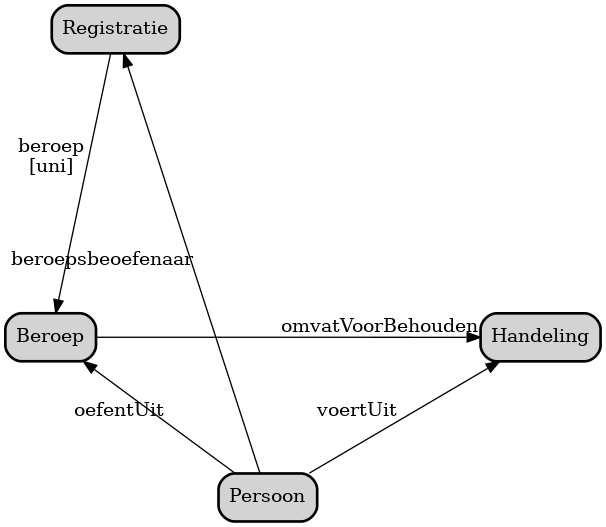
\includegraphics[scale=0.4]{CDConceptBeroep.png}
\centering
\caption{relations}
\label{fig:relations}
\end{figure}
The multiplicity must also be determined for each relation.
\begin{table}[h!]
    \begin{tabular}{||l | l||} 
     \hline
    function & The corresponding control question for the above relation $voerUit$ is\\
    \hline\hline
        Univalent & For each $Persoon$ there is at most 1 $Handeling$\\ %elke P max 1 H
        Total & For each $Persoon$ there is at least 1 $Handeling$ \\ %elke P minimaal 1 H
        Injective & For each $Handeling$ there is only 1 $Persoon$\\ %elke H max 1 P 
        Surjection & For each $Handeling$ there is at least 1 $Persoon$\\ %elke H minimaal 1 P
    \end{tabular}
    \caption{multiplicity}
    \label{tab:multiplicity}
\end{table}

By modelling using the Ampersand method, the question can be answered whether Ampersand provides more insight into the relationships.
As part of the research question, Ampersand can help you gain insight into the relationships.
Although you have to recognize and define these yourself, Ampersand will be helpful in generating functional design and prototype.
The generated prototype will validate the named constraints.
This will prevent registrations that do not meet the constraints.
These constraints are laid down in rules within Ampersand.
For example, a rule can be drawn up that determines whether a person is allowed to perform a certain action.
In figure \ref{fig:relations} the relations are named.
It was previously established that there are 2-tuple relationships.
Here we use the following notation:"$\mathit{relation [Concept \times Concept]}$".
\begin{center}
$\mathit{voertUit [Persoon \times Handeling]}$ ; 
 $\mathit{omvatVoorBehouden [Beroep \times Handeling]~\smallsmile}$
\newline $\subseteq$
\newline $\mathit{beroepsbeoefenaar [persoon \times registratie]}$ ;
$\mathit{beroep [registratie \times beroep]}$
\end{center}
The compared sets are
\newline $\mathit{[Persoon \times Beroep]}$
\newline The rule then will determine if the previous equation is true.
\newline If this is the case, then the rule is validated, otherwise the violation message occurs.
\begin{lstlisting}
    RULE HandelingDoorPersoon: voertUit; omvatVoorBehouden[Beroep*Handeling]~ |- beroepsbeoefenaar; beroep
    MEANING "Een persoon mag handelingen uitvoeren wanneer hij een bepaald beroep uitoefend"
    MESSAGE "Geen toegestane handeling."
    VIOLATION (TXT "Persoon ", SRC I, TXT " voert de handeling uit ", TGT I, TXT " die niet tot zijn beroep behoren ", SRC I[Persoon];oefentUit)
\end{lstlisting}


\subsection{Reactive approach} \label{reactive_approach}

The start of the reactive approach started with the reactive manifesto~\citepNonPub{reactive_manifesto}.
This defines the aspects that a reactive system should meet.
This includes Responsive, Resilient, Elastic and Message Driven.
These are systems that are flexible, loosely coupled and scalable and that makes them easier to develop and maintain.
Reactive Systems are made highly responsive and provide interactive feedback.
\begin{figure}[H] 
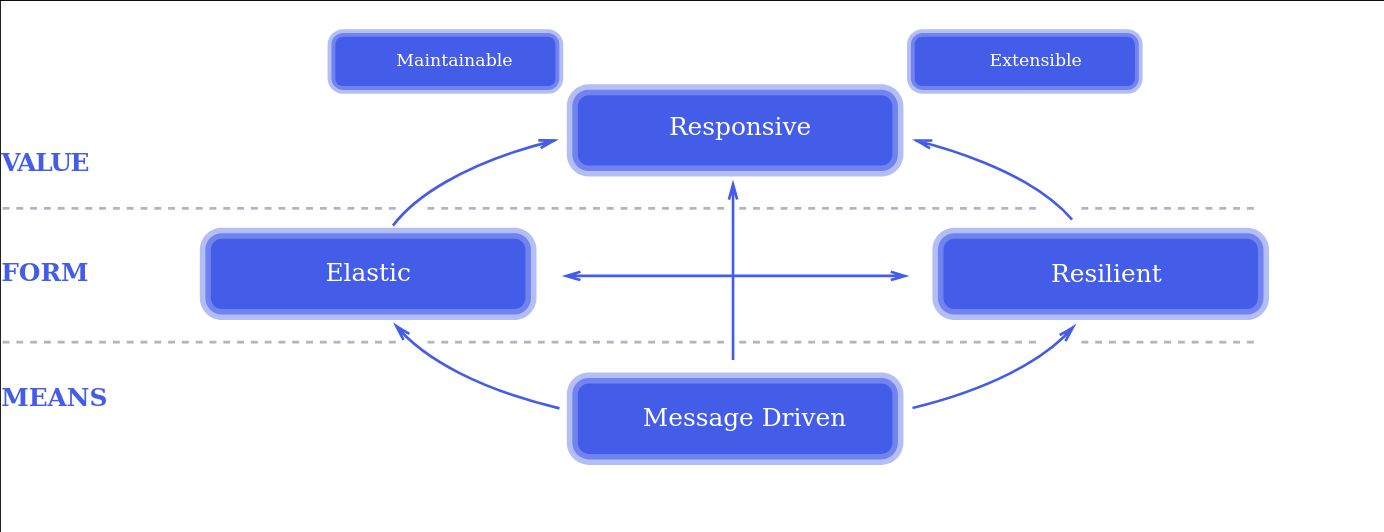
\includegraphics[scale=0.3]{reactive_manifesto.png}
\centering
\caption{reactive manifesto}
\label{fig:reactive manifesto}
\end{figure}


Ampersand is a form of Functional Reactive Programming (FRP)~\citep{elliott_functional_1997}.
The basic of reactive programming is the fact that it involves asynchronous communication.
This means that, as the \citeNonPub{reactive_manifesto} prescribes, use is made of message driven systems, but Ampersand is more than a message-driven system.
It is actually an event-driven system.
The glossary of the \citeNonPub{reactive_manifesto} indicates the difference between message driven systems and event driven systems.
An event-driven system targets event-bus while a message-driven system targets recipients~\citep{bainomugisha_survey_2013}.
The essence is that the order of the flow cannot be determined in advance.
The system will respond to events caused by constraints, Ampersand determines a dynamic flow~\citep{joosten_relation_2018}.




\subsubsection{Law analysis} \label{law_analysis}
The tax authorities have developed a method that is intended to analyse tax laws and other laws.
This is performed in these 6 steps:
\begin{enumerate}
    \item Determining the work area.
    \item Making the structure visible in legislation.
    \item Defining the meaning of legislation.
    \item Validate the analysis results.
    \item Identify missing execution policy.
    \item Setting up the knowledge model.
\end{enumerate}
Emphasis is placed on the cooperation between the implementer, ICT and policy.
By going through the method step by step, one arrives at a shared language.
This shared language includes the definition of concepts by the collaborating parties.
An important part of the approach is dividing the law into small pieces and always refer to these pieces of law in the implementation.
As a result, the method meets the requirement of the justification of government decisions.
The decisions are traceable, explainable, and it is possible to account for them.
What is not clear from the webinar~\citeNonPub{belastingdienst_webinar_2021} is how these steps were converted into an implementation.
The book~\citeNonPub{ausems_wetsanalyse_2021} indicates that the legal analysis method does not contain a development tool, but that the Tax and Customs Administration has developed an instrument based on the legal model, which is not freely available.


%\subsection{Design method} \label{design_method}
The method used in this study is the Ampersand method.
The Ampersand method is based on relational algebra.
Ampersand makes it possible to make a conceptual analysis of problems. The data model created thereby makes it possible to accelerate implementation.


\subsubsection{Relation Algebra} \label{relation_algebra}
The field of the relation algebra, founded by De Morgan, focuses on operations with sets.
The signature item of relational algebra is the relationship, as the name implies.
This relationship has several properties, namely the attributes.
The attributes in the example of \acrshort{big} would be the surname, first names, gender, date of birth, nationality and address of the person concerned and the number and time of registration~\footnote{\acrlong{big} article 3, paragraph 2}.
In addition, the relationship consists of tuples.
Since the relationship is always between two objects, this is called 2-tuples.
The tuples contain the attributes of the relation.

Basically the operations on sets are the following:
\begin{itemize}
    \item Union, $R \cup S$ %vereniging
    \item Intersection, $R \cap S$ %doorsnede
    \item Difference, $R - S$ or $S - R$ %verschil
\end{itemize}
A distinction must be made between relation algebra and relational algebra.
Ampersand uses relation algebra, so is tuple related and the relational algebra is the foundation of e.g. relational databases.
This includes projections, selections and joins.
The latter are therefore not part of relation algebra.


\subsubsection{Ampersand} \label{ampersand}
Ampersand is based on relation algebra and focuses on business rules~\citepNonPub{wedemeijer_l_joosten_smm_michels_garkenbout_jlc_werkboek_ontwerpen_met_bedrijfsregelspdf_nodate}.
Ampersand supplies correct information systems.
In this case, Ampersand's goal is to provide a correct registry system.
Ampersand's other strengths are its support for conceptual analysis.
It is a platform for reactive programming and generates prototypes.
Ampersand describes the goals rather than the steps.

Business rules are there to pursue a common goal.
These rules are converted into an information system. 
The Ampersand method ensures that when a precise set of rules has been established, an information system can be generated. 
Ampersand focuses on business rules.
To learn how Ampersand works in real life, we design a registry in Ampersand that implements the \acrshort{big}~\citepNonPub{van_wet_2018} .

\begin{wrapfigure} {r}{0.52\textwidth} 
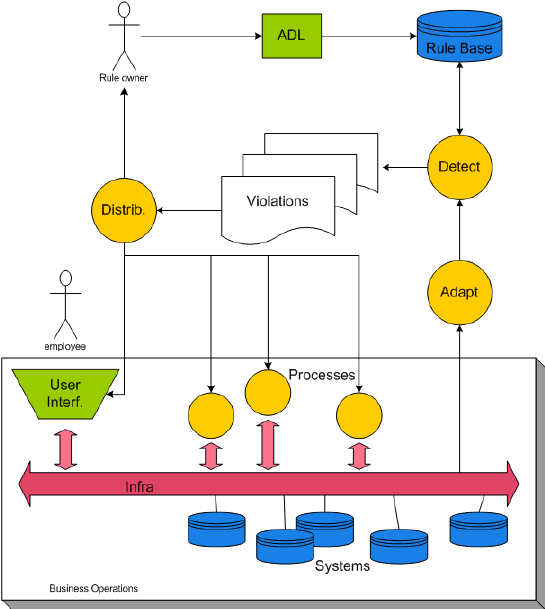
\includegraphics[width=7cm, height=6cm]{Principle-of-rule-based-process-management.png}
\caption{rule-based-proces}
\label{fig:rule-based-proces}
\end{wrapfigure}


The principle of rule-based \acrfull{bpm} as mentioned in \citepNonPub{joosten_joosten} is that any violation of a business rule may be used to trigger actions. 
This is described in the section \nameref{reactive_approach}.

Ampersand consists of concepts that in turn consist of atoms.
An atom is an implementation of the concept.
Inside the \acrshort{big} is a concept "beroep" with associated atoms like "arts, tandarts, etc".
The concepts are given a name, and the name must be recognized by the business.
This also applies to the definition and purpose of the concepts.
These attributes are not mandatory, but when one wants to generate a functional design, these descriptions of the attributes are very useful.
\begin{lstlisting}[language=Octave] 
CONCEPT Beroep "Beroep van een persoon zoals bedoeld in de wet" 
PURPOSE CONCEPT Beroep 
{+Beroep dat uitgeoefend wordt+}
POPULATION Beroep CONTAINS [
    "arts",
    "tandarts",
    "apotheker",
    "gezondheidszorgpsycholoog",
    "psychotherapeut",
    "fysiotherapeut",
    "verloskundige",
    "verpleegkundige",
    "physician assistant",
    "orthopedagoog-generalist"
]
\end{lstlisting}

Concepts can have relationships with each other.
If the data of the concepts is true and the rules yield consistent data then the relationships between real data are facts.
These facts together form one truth.
Not all concepts are directly related.
Within the domain of the \acrshort{big} we could distinguish the concept of "registratie" and the concept of "beroep".
This name is also referred to within ~\citeNonPub{van_wet_2018} in article 3 of \acrshort{big}.
Even the name of the relationship is mentioned in this article, which the legislator calls a "beroepsbeoefenaar".
The law requires that data of the "registratie" be recorded, indicating the corresponding profession (beroep).
In Ampersand, this is modelled as follows.
On the one hand, the "beroep" and also the concept "registratie".
\begin{lstlisting}[language=Octave] 
    CONCEPT Registratie "De registratie van een persoon binnen het register" 
    PURPOSE CONCEPT Registratie 
    {+Vastlegging in het register geeft toegang tot uitoefenen taak binnen de gezondheidszorg+}
\end{lstlisting}
Between the "registratie" and the $persoon$ exists the relationship "beroepsbeoefenaar".
\begin{lstlisting}[language=Octave] 
RELATION beroepsbeoefenaar [Persoon*Registratie] 
MEANING "geregistreerd persoon"
POPULATION beroepsbeoefenaar CONTAINS 
[
  ("Piet",1);
  ("Susan",2);
  ("Gerard",3);
  ("John",4)
]\end{lstlisting}
Also adding the concepts of $persoon$ and $handeling$.
Persons may perform the medical actions, but only when they are qualified.
\begin{lstlisting}[language=Octave] 
    CONCEPT Persoon "Persoon die werkzaam wilt zijn binnen de zorg"
    PURPOSE CONCEPT Persoon 
    {+Vastleggen van de identiteit van de persoon+}
\end{lstlisting}
\begin{lstlisting}[language=Octave] 
    CONCEPT Handeling "Acties die uitgevoerd worden" 
    PURPOSE CONCEPT Handeling 
    {+Vastleggen van de mogelijke handelingen die uitgevoerd kunnen worden binnen de zorg+}
\end{lstlisting}
These concepts can lead us to the following scheme.
\begin{figure}[H] 
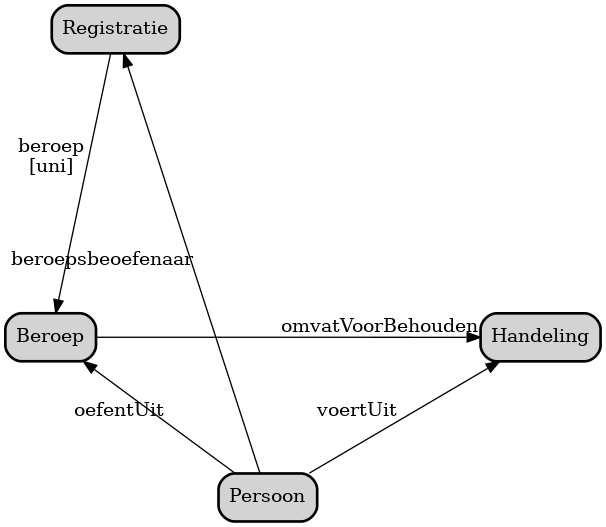
\includegraphics[scale=0.4]{CDConceptBeroep.png}
\centering
\caption{relations}
\label{fig:relations}
\end{figure}
The multiplicity must also be determined for each relation.
\begin{table}[h!]
    \begin{tabular}{||l | l||} 
     \hline
    function & The corresponding control question for the above relation $voerUit$ is\\
    \hline\hline
        Univalent & For each $Persoon$ there is at most 1 $Handeling$\\ %elke P max 1 H
        Total & For each $Persoon$ there is at least 1 $Handeling$ \\ %elke P minimaal 1 H
        Injective & For each $Handeling$ there is only 1 $Persoon$\\ %elke H max 1 P 
        Surjection & For each $Handeling$ there is at least 1 $Persoon$\\ %elke H minimaal 1 P
    \end{tabular}
    \caption{multiplicity}
    \label{tab:multiplicity}
\end{table}

By modelling using the Ampersand method, the question can be answered whether Ampersand provides more insight into the relationships.
As part of the research question, Ampersand can help you gain insight into the relationships.
Although you have to recognize and define these yourself, Ampersand will be helpful in generating functional design and prototype.
The generated prototype will validate the named constraints.
This will prevent registrations that do not meet the constraints.
These constraints are laid down in rules within Ampersand.
For example, a rule can be drawn up that determines whether a person is allowed to perform a certain action.
In figure \ref{fig:relations} the relations are named.
It was previously established that there are 2-tuple relationships.
Here we use the following notation:"$\mathit{relation [Concept \times Concept]}$".
\begin{center}
$\mathit{voertUit [Persoon \times Handeling]}$ ; 
 $\mathit{omvatVoorBehouden [Beroep \times Handeling]~\smallsmile}$
\newline $\subseteq$
\newline $\mathit{beroepsbeoefenaar [persoon \times registratie]}$ ;
$\mathit{beroep [registratie \times beroep]}$
\end{center}
The compared sets are
\newline $\mathit{[Persoon \times Beroep]}$
\newline The rule then will determine if the previous equation is true.
\newline If this is the case, then the rule is validated, otherwise the violation message occurs.
\begin{lstlisting}
    RULE HandelingDoorPersoon: voertUit; omvatVoorBehouden[Beroep*Handeling]~ |- beroepsbeoefenaar; beroep
    MEANING "Een persoon mag handelingen uitvoeren wanneer hij een bepaald beroep uitoefend"
    MESSAGE "Geen toegestane handeling."
    VIOLATION (TXT "Persoon ", SRC I, TXT " voert de handeling uit ", TGT I, TXT " die niet tot zijn beroep behoren ", SRC I[Persoon];oefentUit)
\end{lstlisting}


\subsection{Reactive approach} \label{reactive_approach}

The start of the reactive approach started with the reactive manifesto~\citepNonPub{reactive_manifesto}.
This defines the aspects that a reactive system should meet.
This includes Responsive, Resilient, Elastic and Message Driven.
These are systems that are flexible, loosely coupled and scalable and that makes them easier to develop and maintain.
Reactive Systems are made highly responsive and provide interactive feedback.
\begin{figure}[H] 
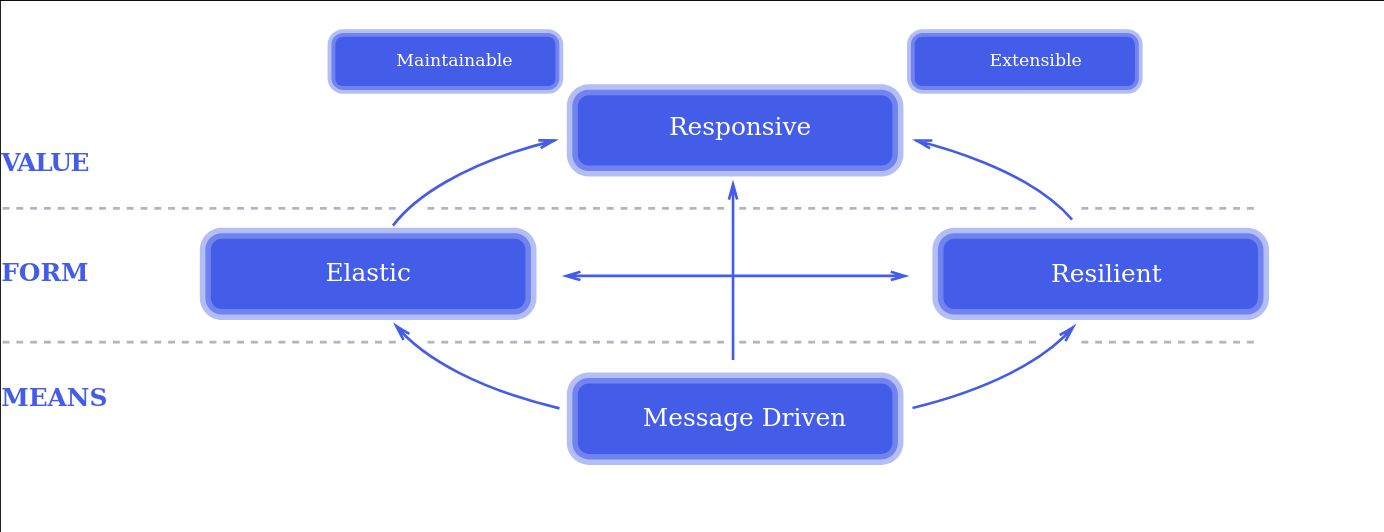
\includegraphics[scale=0.3]{reactive_manifesto.png}
\centering
\caption{reactive manifesto}
\label{fig:reactive manifesto}
\end{figure}


Ampersand is a form of Functional Reactive Programming (FRP)~\citep{elliott_functional_1997}.
The basic of reactive programming is the fact that it involves asynchronous communication.
This means that, as the \citeNonPub{reactive_manifesto} prescribes, use is made of message driven systems, but Ampersand is more than a message-driven system.
It is actually an event-driven system.
The glossary of the \citeNonPub{reactive_manifesto} indicates the difference between message driven systems and event driven systems.
An event-driven system targets event-bus while a message-driven system targets recipients~\citep{bainomugisha_survey_2013}.
The essence is that the order of the flow cannot be determined in advance.
The system will respond to events caused by constraints, Ampersand determines a dynamic flow~\citep{joosten_relation_2018}.




\subsubsection{Law analysis} \label{law_analysis}
The tax authorities have developed a method that is intended to analyse tax laws and other laws.
This is performed in these 6 steps:
\begin{enumerate}
    \item Determining the work area.
    \item Making the structure visible in legislation.
    \item Defining the meaning of legislation.
    \item Validate the analysis results.
    \item Identify missing execution policy.
    \item Setting up the knowledge model.
\end{enumerate}
Emphasis is placed on the cooperation between the implementer, ICT and policy.
By going through the method step by step, one arrives at a shared language.
This shared language includes the definition of concepts by the collaborating parties.
An important part of the approach is dividing the law into small pieces and always refer to these pieces of law in the implementation.
As a result, the method meets the requirement of the justification of government decisions.
The decisions are traceable, explainable, and it is possible to account for them.
What is not clear from the webinar~\citeNonPub{belastingdienst_webinar_2021} is how these steps were converted into an implementation.
The book~\citeNonPub{ausems_wetsanalyse_2021} indicates that the legal analysis method does not contain a development tool, but that the Tax and Customs Administration has developed an instrument based on the legal model, which is not freely available.

\newpage
\newpage
\printglossary


%\nocite{*}
\bibliographystyle{plainnat}
\bibliographystyleNonPub{plainnat}
\bibliography{00_common/report}
\bibliographyNonPub{00_common/reportNonPub}

%appendix
\newpage
\appendix

\section{Observations} \label{appendixLoglines}
\def\rq{RQ1}
\cntA{Ampersand}
\cntA{api}
\cntA{classify}      
\cntA{concept}   
\cntA{Conceptual analysis}
\cntA{concepten}     
\cntA{crud}           
\cntA{Docker}   
\cntA{documentation}
\cntA{flexible}     
\cntA{include}
\cntA{interface}     
\cntA{latex}
\cntA{Lifecycle}
\cntA{linkto}        
\cntA{multiplicity}  
\cntA{Obsidian}
\cntA{pattern}
\cntA{php}
\cntA{population}    
\cntA{prototype}
\cntA{RAP}            
\cntA{relation}
\cntA{represent}      
\cntA{rule}
\cntA{VSC}
\cntA{XML}
\cntA{JSON}
\cntA{RTF}
\cntA{PDF}
\cntA{validation}
\cntA{architecture}

\acrlong{\rq}

\paragraph{Ampersand}
\begin{enumerate}
    \item rq1-13:17-10: The setup of \A{Ampersand} in local environment is specific and not self-explanatory.
    Help is needed here to get this working.
    Attempts to get the process working in localhost were unsuccessful.
    The manual on the Ampersand site showed how to do this.
    But it still didn't work
    \newline\textbf{obs}: the documentation gives an indication of how to configure ampersand and make it work locally.
    Using XAMP.
    All this is not going to work.
    Not clear why.
    It did work in a Docker environment.

    \item rq1-18 Can not find an example on the internet, only in the repo of \A{Ampersand} itself.
    That is difficult to find.
    \newline\textbf{obs}: Little to be found about Ampersand except in its own repos.

    \item rq1-45:24-10: Overview within a \A{Ampersand}script is difficult to maintain and obtain.
    \newline\textbf{obs}: The need for overview is there as the script grows.

    \item rq1-2 \A{Ampersand} has no annotation option, therefore requires a separate action or document to keep track of what has been passed.
    \newline\textbf{obs}: it comes down to wanting to maintain an overview. 
    That is what I want with the annotation.

    \item rq1-47:27-10: Detecting a bug.
    Placing these in github issues at the \A{Ampersand} repository will get a response within a day and resolve it.
    In this case it was a bug in Ampersand that was quickly fixed with a new version.
    \newline\textbf{obs}: Quick fix of a bug in Ampersand by the development team.

    \item rt1-60:9-11: The process of writing a \A{Ampersand} script is not without practice.
    \newline\textbf{obs}: There should always be someone with experience in the background or in the collaboration.

    \item rq1-96:30-12: Skill in scripting within \A{Ampersand} is quickly lost if you don't do this frequently.
    \newline\textbf{obs}: Practice a lot and keep using it.

\end{enumerate}

\paragraph{Api}
\begin{enumerate}
    \item rq1-8:14-11: No swagger is created for the \A{api};
    \newline\textbf{obs}: If you want to use an external input, API descriptions are very relevant.
    These are not generated automatically.
    
    \item rq1-70:14-11: Postman works with api/v1/resource, e.g. GET \url{localhost/api/v1/resource/Person/P001/Person}, retrieves that of an existing person.
    So the validation structure of ampersand can be used from outside Ampersand by means of \A{api}.
    \newline\textbf{obs}: Ampersand is more open than it first appears.

    \item rq1-72:14-11: Besides the GET(get), the POST(append) and PUT (mutate) also work
    \newline\textbf{obs}: Using Postman, the \A{api} features were tested.
    
    \item rq1-73:14-11: Ampersand can be used from other applications through \A{api}'s, but the return values are next to the requested information also messages and not message codes.
    These codes could be included in the reports, but now remain "unstructured" data.
    \newline\textbf{obs}: Here you are missing the structure of the responses.
    So Ampersand is apparently not intended to be used in this way.
    See also note on swagger(rq1-8).
    
    \item rq1-74:16-11: Link between an external front-end and an Ampersand back-end (Ampersand\-\A{api}).
    A change in the back-end, so an Ampersand change, then the front end almost certainly has to change with it.
    \newline\textbf{obs}: Forced maintenance of the external front-end due to changes within Ampersand APIs.

\end{enumerate}

\paragraph{Architecture}
\begin{enumerate}
    \item rq1-62:10-11: There has be the \A{architecture} link between the {law core} and the {register core}
    \newline\textbf{obs}: Ampersand analysis must fit the architecture of the organization and the way of working.

\end{enumerate}

\paragraph{Classify}
\begin{enumerate}
    \item rq1-86:30-11: \A{classify} is a specialization of a concept.
    No experience has been gained with this.
    \newline\textbf{obs}: There was no place for this in the research.

\end{enumerate}

\paragraph{Concept}
\begin{enumerate}
    \item rq1-16 Notation method of \A{concept} and {relation}s and {rule}s are defined for a very small part.
    Only the first position is uppercase or lowercase.
    There is no rule about other spelling.
    So using CamelCase or underscore or hyphen.
    \newline\textbf{obs}: You are not forced to work in any particular structure.
    There is no need for coercion in this area, but advice is practical for novice users.
     
    \item rq1-79:20-11: Once the \A{concept} Define date and then it can be used anywhere in the context.
    The question then is how to deal with shared Concepts and how to manage them.
    \newline\textbf{obs}: Within the context, a concept is reused.
    The operation of shared concept within other contexts is not self-evident.
     
    \item rq1-30:12-9: Defining the meaning and definition of the \A{concept} is free.
    There is no fixed pattern for documentation.
    \newline\textbf{obs}: Defining the meaning and definition is very free.
     
    \item rq1-42:19-10: Immediately add the description when recording a \A{concept} and {relation}.
    Later it is difficult to find out why the recording took place.
    \newline\textbf{obs}: To avoid rework, the definition and meaning and purpose should be defined immediately when defining concepts and relationships.

    \item rq1-48:27-10: The \A{concept} current date is solved very complicated.
    But eventually it works.
    Current time does not seem to have developed yet.
    Although the example scripts seem to say something different.
    \newline\textbf{obs}: A frequently used element like date and time is not easily solved in Ampersand.
    
    \item rq1-46:24-10: There is no find able relationship between the {relation} and the \A{concept} in the script.
    \newline\textbf{obs}: The {overview} where a concept is used is difficult to obtain.
    The IDE used also does not provide any tooling to obtain this overview.

    \item rq1-80:20-11: A consistent naming of a \A{concept} is necessary.
    \newline\textbf{obs}: A once defined concept could just be redefined (due to lack of overview).
    With just a different format or definition.
    
    \item rq1-84:30-11: A \A{concept} is immutable.
    for example a person is concept, not doctor.
    It must be an intrinsic property, which cannot be changed.
    \newline\textbf{obs}: The important property of concept within Ampersand.
    
    \item rq1-89:7-12: Items named as common \A{concept}s.
    \newline\textbf{obs}: There are common elements across registers. The question is how to address this commonality.
    
    \item rq1-91:14-12: A \A{concept} and a {relation} can be defined several times within your own patterns.
    So that the patterns can stand on their own.
    \newline\textbf{obs}: Dangerous because it allows the same concepts to have different definitions.
\end{enumerate}

\paragraph{Conceptual analysis}
\begin{enumerate}
    \item rq1-1 Formatting in Ampersand ({pattern}s) has consequences for the \A{Conceptual analysis}.
    \newline\textbf{obs}: \textbf{\textit{**welke dan ?? nog even over nadenken**}}
    
    \item rq1-43:23-10: The order of the data in the \A{Conceptual analysis} is a bit strange.
    First the definition is shown, then the name of the relation and below that the meaning again.
    \newline\textbf{obs}: The layout of the Conceptual design doesn't seem quite logical and is therefore confusing.

    \item rq1-44:23-10: In the \A{Conceptual analysis} enters must be taken into account in the texts.
    These come back directly in the documents and then yield broken sentences.
    \newline\textbf{obs}: Break enters in the \acrshort{ide} also produce extra newlines in the output.
    This causes the formatting to go wrong.

    \item rq1-76:20-11: The "disclaimer" does not appear in the \A{Conceptual analysis}.
    \newline\textbf{obs}: The "disclaimer" does not appear in the Conceptual analysis.

    \item rq1-99:6-1: when generating a \A{Conceptual analysis} the doc gets the name of the first concept.
    \newline\textbf{obs}: The name of the generated document will be the name of the first draft contained in the document.

    \item rq1-35:14-9: The law has been drawn up in Dutch, which means that the \A{Conceptual analysis} can also be done in Dutch.
    \newline\textbf{obs}: The starting point is to make the Conceptual analysis in Dutch.

    \item rq1-51:2-11: Discussing the \A{Conceptual analysis} should be done theme by theme.
    \newline\textbf{obs}: Where a theme equals pattern.

\end{enumerate}

\paragraph{\acrlong{crud}}
\begin{enumerate}
    \item rq1-53:2-11: The \A{crud} (\acrlong{crud}) and \acrshort{crud} in the {interface} don't always work as it should be.
    There is no full validation on usage.
    So an on/off does not make sense everywhere.
    \newline rq1-37:3-10: CRUD/crud options also need some study before they can be applied properly.
    \newline\textbf{obs}: No (full) validation on the use of crud.
    It is possible to apply variations that have no impact.

\end{enumerate}

\paragraph{Docker}
\begin{enumerate}
    \item rq1-11 Implementation in \A{Docker} with RAP creates new directories all the time.
    \newline\textbf{obs}: The Docker environment is polluted by adding new directories all the time.
    This makes analysis difficult because it is not clear which directory is used.

    \item rq1-6:21-10/30-10: \A{Docker} is also another thing to learn.
    There should also be an introductory course to quickly understand Docker usage for Ampersand.
    A waste of time to have to look this up yourself or it is preconditions to be able to use Ampersand.
    \newline\textbf{obs}: Docker knowledge (limited) is required

    \item rq1-49:30-10: Isolating a {pattern} or subsystem for testing does not work.
    This has to do with setting up \A{Docker} and possible ignorance on my part.
    \newline\textbf{obs}: The goal was to put a part of the system on its own so that only that part could be tested.
    But due to the Docker setup, this doesn't seem possible.
    Or I don't have enough knowledge of Docker to make this possible.

\end{enumerate}

\paragraph{Documentation}
\begin{enumerate}
    \item rq1-78:20-11: The \A{documentation} generated in HTML loaded in firefox and no PNG's are visible.
    Chrome is doing well.
    \newline\textbf{obs}: Firefox does not show the generated models.

    \item rq1-41:19-10: The law bank website contains a persistent hyperlink, which can be used in the \A{documentation} as reference.
    \newline\textbf{obs}: References to persistent links can be included.
    But is the output still pleasant to read because of the continuous references.

    \item rq1-54:2-11: The \A{documentation} can be written in different ways.
    This can be done using mark down, html and latex.
    \newline\textbf{obs}: You will encounter this in usage, even though the documentation states this as well.

    \item rq1-97:30-12: By puzzling with Ampersand people quickly forget to make correct \A{documentation}.
    Often you are happy that something works.
    \newline\textbf{obs}: Too much trying and figuring distracts from documenting.

    \item rq1-75:20-11: Some more experimentation with the \A{documentation} in the prototype.
    When describing the purpose of the context, it takes a while to figure out how this text can be properly conveyed.
    An <h1> results in an extra chapter in H4 and H4 then becomes H5. And H5 has then become a meaningless piece.
    With an <h2> and <h3> it works well.
    \newline\textbf{obs}: Interfering with structure can have unexpected consequences.

\end{enumerate}

\paragraph{Flexible}
\begin{enumerate}
    \item rq1-63:10-11: Ampersand is \A{flexible} by extension concepts and relationships.
    Such as dividing an address into street name, house number and addition is quickly realized.
    Actual address formatting is not in the law.
    The usual method within the government is to conform to BRP use of addresses.
    \newline\textbf{obs}: Ampersand is very flexible.
    Define a Concept and relationship and it is realized.
    Second observation is that in the case of the address it is not immediately clear what this should look like.
    But there are other sources for that.
    It takes some searching and making assumptions.

\end{enumerate}

\paragraph{Include}
\begin{enumerate}
    \item rq1-81:20-11: Compilation error due to a \A{include} that no longer existed.
    Observation here is that an adl has been renamed or moved or deleted.
    The tool \acrlong{vsc} does not support a refactoring stroke on said changes.
    \newline\textbf{obs}: Refactoring is not supported with \acrlong{vsc}.

    \item rq1-15:4-10 With \A{include} statements the order of the contents of the document is determined.
    The expectation was that includes are needed to link parts of code together but includes are not everywhere necessary to get the code working.
    \newline\textbf{obs}: Includes are not only to run the scripts completely, but also to send the documentation.

    \item rq1-82:20-11: \A{include} don't always seem necessary on compilation.
    It is not entirely clear when this is necessary or not.
    Another function of includes is to format the analysis.
    \newline\textbf{obs}: Includes are useful and necessary, but it's not always clear how to use them.

    \item rq1-90:14-12: Collection model of regulations than by means of \A{include}s keep it small and therefore clear.
    This is for the reusability of the script.
    One module per feature.
    \newline\textbf{obs}: Small modules with reusability in mind.

\end{enumerate}
 
\paragraph{Interface}
\begin{enumerate}
    \item rq1-12 At the start it is not clear when a capital letter or small letter should be used with the crud in the \A{interface}.
    \newline\textbf{obs}: It is in the manual\footnote{\url{https://ampersandtarski.gitbook.io/documentation/the-language-ampersand/services/crud}}, 
    but you have to find out by trial and error how it really works.
    
    \item rq1-40:10-10/27-11: The concepts used in the \A{interface} must be of type "object" (represent).
    The concept may therefore not be alpha or integer.
    \newline\textbf{obs}: Interface did not start correctly.
    This was caused by the interface concept not being of type "object".

    \item rq1-53:2-11: The {crud} (\acrlong{crud}) and \acrshort{crud} in the \A{interface} don't always work as it should be.
    There is no full validation on usage.
    So an on/off does not make sense everywhere.
    \newline rq1-37:3-10: CRUD/crud options also need some study before they can be applied properly.
    \newline\textbf{obs}: No (full) validation on the use of crud.
    It is possible to apply variations that have no impact.

    \item rq1-58:8-11: Per \A{interface} max 1 {multiplicity}, otherwise you won't get data stored.
    \newline\textbf{obs}: Within an interface, multiple total constraints were included in the relationships.
    The result was that no more data could be added within the prototype.

    \item rq1-71:14-11/16-11: The \A{interface} also belongs to the design and not just to the prototype.
    Changing the \acrlong{crud} changes the behavior of the API.
    \newline\textbf{obs}: API behavior changes by changing \acrshort{crud}.

    \item rq1-83:27-11: Experiment with HTML view within the \A{interface} fails.
    Documentation of this is not conclusive.
    The examples are not enough
    \newline\textbf{obs}: This part was not made to work.    

    \item rq1-98:30-12: When using {linkto} in the \A{interface} as last element in the interface and the signature occurs more often than a dropdown to all subinterfaces (of the same signature) appears.
    \newline\textbf{obs}: Unexpected behavior of the LINKTO.
    
    \item rq1-5:30-10: The browser is holding data from the \A{interface} and periodically the cache needs to be cleared for customization to work.
    \newline\textbf{obs}: It looks like the changes made to the script don't affect operation.
    It is caused by the browser's cache not being emptied automatically.
    There are browser extensions to still do this manually.

    \item rq1-10 The function html href with target blank does not work within the \A{interface}
    \newline rq1-77:20-11: In html mode the 
    \begin{lstlisting}
    <a href="x" target=\_blank>
    \end{lstlisting}
    is not supported.
    The target is removed in the complation.
    \newline\textbf{obs}: The expectation was that the target \_blank would open a new tab in the html text, but that does not happen.
    
\end{enumerate}

\paragraph{Latex}
\begin{enumerate}
    \item rq1-33:9-1: \A{VSC} does not support the \A{latex} environment well.
    My PC often hangs on this.
    \newline rq1-87:3-12: Latex can also be written in VSC.
    Apparently it is a different version, because the import does not immediately succeed.
    Does not work really well and the result is poor.
    \newline\textbf{obs}: \acrlong{vsc} also supports the TEX environment through add-ons.
    But this add-on completely hangs my system.
    I got a 100\% cpu load for a long time. 


\end{enumerate}

\paragraph{Lifecycle}
\begin{enumerate}
    \item rq1-39:3-10: Do not forget to create delete rules in addition to append and edit rules in the {rule}\textbf{s} in the context of the \A{Lifecycle} approach.
    \newline\textbf{obs}: Completeness of functions on the relations.

\end{enumerate}

\paragraph{Linkto}
\begin{enumerate}
    \item rq1-98:30-12: When using \A{linkto} in the {interface} as last element in the interface and the signature occurs more often than a dropdown to all subinterfaces (of the same signature) appears.
    \newline\textbf{obs}: Unexpected behavior of the LINKTO.
    

\end{enumerate}

\paragraph{Multiplicity}
\begin{enumerate}
    \item rq1-58:8-11: Per \A{interface} max 1 \A{multiplicity}, otherwise you won't get data stored.
    \newline\textbf{obs}: Within an interface, multiple total constraints were included in the relationships.
    The result was that no more data could be added within the prototype.

    \item rq1-66:10-11: XLSX files format is created partly on the basis of \A{multiplicity}.
    1 on n relation produces its own tab.
    \newline\textbf{obs}: The Excel file is a reflection of the database structure so that insight can be obtained in the database structure.

    \item rq2-5:2-10: Making the \A{multiplicity} explicit.\newline
    \begin{tabular}{ || l | l | l ||}
    \hline
    UNI & P->0-1 H &  most\\  \hline    
    TOT & P->1-* H  & least\\  \hline
    INJ & H->1 P  &   one\\  \hline
    SUR & H->1-* P &  at least 1\\ \hline
    \end{tabular}
    \newline\textbf{obs}: Since you don't always have a clear picture of how this works, it needs to be written out to make it workable.
    
    \item rq1-3 Created a separate excel to write out and discover the \A{multiplicity} of the relations.
    \newline\textbf{obs}: As a method this is a clear way.
    Did notice that it is difficult (from a management perspective) to keep the Excel document in sync with the scripts.

\end{enumerate}

\paragraph{Obsedian}
\begin{enumerate}
    \item rq1-88:5-12: Tried the tool \A{Obsidian} as a new tool.
    But here too I do not get an immediate overview and it is digital.
    Apparently writing in a log is more convenient for me
    \newline\textbf{obs}: Also tried a new tool while writing the logs.
    Either this one does not work for me or I need to be more patient.

\end{enumerate}

\paragraph{Pattern}
\begin{enumerate}
    \item rq1-1 Formatting in Ampersand (\A{pattern}s) has consequences for the {Conceptual analysis}.
    \newline\textbf{obs}: \textbf{\textit{**welke dan ?? nog even over nadenken**}}
    
    \item rq1-49:30-10: Isolating a \A{pattern} or subsystem for testing does not work.
    This has to do with setting up {Docker} and possible ignorance on my part.
    \newline\textbf{obs}: The goal was to put a part of the system on its own so that only that part could be tested.
    But due to the Docker setup, this doesn't seem possible.
    Or I don't have enough knowledge of Docker to make this possible.

    \item rq1-33:14-9: The use of \A{pattern}s within Ampersand is important.
    These are the subsystems of the information system.
    The question is whether this should be classified in advance or whether it builds up on its own.
    \newline\textbf{obs}: Use of patterns is necessary for the subsystem layout.

    \item rq1-34:14-9: The spelling of a \A{pattern} is capitalized.
    And the pattern ends with an end-pattern.
    Multiple patterns are possible within one script.
    \newline\textbf{obs}: It's in the documentation, but you read about it.
    It must happen to you.

    \item rq1-38:3-10: Should the subsystems be mapped in advance.
    This is controlled via \A{pattern}\textbf{s}.
    \newline\textbf{obs}: It is not necessary to divide the analysis in advance into patterns or subsystems.
    It is possible, but then there must already be a good picture of the text.

\end{enumerate}

\paragraph{PDF, RTF, XML, JSON}
\begin{enumerate}
    \item rq1-24 12-9/14-9 \A{XML} download from wetBig seems like a logical step for the analysis and processing, but it is too complex.
    This also applies to the JSON structure.
    Both structures are not pleasant to read.
    The thought that comes to mind here is why SDU doesn't directly annotate the concepts and relationships.
    \newline\textbf{obs}: Both structures have been downloaded to add the annotations to them.
    To later use a program to extract the annotation (xml/json annotations) together with the definitions and meaning and to generate a script or part of a script with this.

    \item rq1-31:14-9: Besides \A{XML} and {JSON}, {RTF} and {PDF} are also an option.
    In rtf (doc) you can add items in the margins via "comments".
    With a PDF, annotations and color highlighting can be given this feature.
    \newline\textbf{obs}: To get the overview and to keep track of what has already been processed.
    
\end{enumerate}

\paragraph{Php}
\begin{enumerate}
    \item rq1-9 Adding pieces of \A{php} code in the script is possible, but it is not clear how
    \newline\textbf{obs}: Information is missing  on how to do this.
     
    \item rq1-57-2:7-11: Parts like next big number or now() and today() are better solved in a dev language, like \A{php}.
    \newline\textbf{obs}: A development language like php because it's in the Ampersand software stack.

\end{enumerate}

\paragraph{Prototype}
\begin{enumerate}
    \item rq1-36:29-9: Failed to run \A{prototype} under localhost in Windows\-10.
    The service would not start in localhost.
    We did manage to get the service running within Docker.
    There was an error in the installation documentation.
    Turns out that is was not the installation directory RapInstall, but the directory RAP.
    \newline\textbf{obs}: Unable to run the service in localhost, but within Docker.

    \item rq1-69:14-11: Postman\footnote{\url{https://www.postman.com/product/what-is-postman/}} application installed and works with the \A{prototype}.
    \newline\textbf{obs}: An external resource that can perform tests using api.

    \item rq1-36:3-10: What about \A{prototype} test scenarios.
    \newline\textbf{obs}: Apparently lacking testing tools.
    Generic tools such as Selenium may need to be used.

\end{enumerate}

\paragraph{RAP}
\begin{enumerate}
    \item rq1-11 Implementation in \A{RAP} works, but not with includes.
    \newline\textbf{obs}: By using RAP all the used scripts must be included in one total script.
     
\end{enumerate}

\paragraph{Register}
\begin{enumerate}
    \item rq1-85:30-11: A new structure where the \A{register}s can operate independently of each other, with only the generic elements as common items.
    \newline\textbf{obs}: This does not work due to multicontext issue.

    \item rq1-92:14-12: Basically trying to create its own container per \A{register}.
    Multi-context problem.
    This makes it impossible to isolate these containers.
    \newline\textbf{obs}: It is not possible in the current setup of Ampersand to create your own container per registry.
    
    \item rq1-93:19-12/21-12: Implementation choice for separate \A{register}s has an impact on the whole.
    How to deal with shared modules.
    How to deal with shared data (such as person).
    Should the choice be made to only share the concepts and relationships and not implementation.
    \newline\textbf{obs}: solution could be to provide each register with its own db and a shared db for eg people
    Port usage is therefore an issue.
    Can something be arranged in the .env.
    Elaboration of the own containers does not seem to work, the db structure is always overwritten by the new registry.

\end{enumerate}

\paragraph{Relation}
\begin{enumerate}
    \item rq1-7:10-11: Each \A{relation} is part of a record structure.
    \newline\textbf{obs}: Good to discover how the database structure is established.
    It is probably stated somewhere how this happens.
    But this can be determined through reversed engineering.
    Above all, it provides insight and makes it more tangible.

    \item rq2-11:19-10: An \A{relation} that is univalent is a function.
    A one function there can only come out one thing.
    The description of UNI is therefore P ->0-1 H at most (see 2-5)
    \newline\textbf{obs}: An relation that is univalent is a function.
    
    \item rq1-16 Notation method of {concept} and \A{relation}s and {rule}s are defined for a very small part.
    Only the first position is uppercase or lowercase.
    There is no rule about other spelling.
    So using CamelCase or underscore or hyphen.
    \newline\textbf{obs}: You are not forced to work in any particular structure.
    There is no need for coercion in this area, but advice is practical for novice users.

    \item rq1-42:19-10: Immediately add the description when recording a {concept} and \A{relation}.
    Later it is difficult to find out why the recording took place.
    \newline\textbf{obs}: To avoid rework, the definition and meaning and purpose should be defined immediately when defining concepts and relationships.
    
    \item rq1-91:14-12: A {concept} and a \A{relation} can be defined several times within your own patterns.
    So that the patterns can stand on their own.
    \newline\textbf{obs}: Dangerous because it allows the same concepts to have different definitions.

    \item rq1-46:24-10: There is no find able relationship between the \A{relation} and the {concept} in the script.
    \newline\textbf{obs}: The {overview} where a concept is used is difficult to obtain.
    The IDE used also does not provide any tooling to obtain this overview.

\end{enumerate}

\paragraph{Represent}
\begin{enumerate}
    \item rq1-50:30-10: The \A{represent} statement makes the interface react differently.
    When using the represent statement, the append option ("+") disappears.
    \newline\textbf{obs}: Unexpected behavior, it is not immediately clear why this is happening.

    \item rq1-65:10-11: DATETIME (\A{represent}) field could not be converted to Excel.
    The compilation process hangs on this.
    \newline\textbf{obs}: Crashing while building the application using DATETIME in the represent statement.

\end{enumerate}

\paragraph{Rule}
\begin{enumerate}
    \item rq1-4 Automatically executed \A{rule} are easy to describe, but implementation here also takes a lot of patience and trying.
    \newline\textbf{obs}: Rules are not easy to create.
    To implement rules, knowledge of Ampersand is required and many examples must be used.
    It is usually not possible to immediately implement a rule.
    Many attempts are needed to realize this.

    \item rq1-55:2-11: At the \A{rule} it is necessary to add a ROLE with a MAINTAINS, otherwise the rule will not work.
    \newline\textbf{obs}: In the beginning this is not obvious.
    This becomes clear when studying examples.

    \item rq1-59:9-11: Many messages remain open if not all \A{rule}s are met.
    \newline\textbf{obs}: When the input is handled easily, more and more messages appear.
    The messages are grouped by type.
    The workable screen is getting smaller and smaller.    

    \item rq1-17 Applying a \A{rule}\textbf{s} takes a lot of patience and practice.
    This is quite a steep learning curve.
    \newline\textbf{obs}: Implementing a rule requires knowledge of relation algebra and a lot of trying and looking at examples.

    \item rq1-39:3-10: Do not forget to create delete rules in addition to append and edit rules in the \A{rule}\textbf{s} in the context of the \A{Lifecycle} approach.
    \newline\textbf{obs}: Completeness of functions on the relations.

    \item rq1-67:11-11: If there is an automatic \A{rule}, should there still be a validation rule on it?
    \newline\textbf{obs}: Yes, if there is a chance that the automatic rule is (accidentally) removed or changed.
    Use as an intrinsic control agent.

    \item rq1-16 Notation method of {concept} and {relation}s and \A{rule}s are defined for a very small part.
    Only the first position is uppercase or lowercase.
    There is no rule about other spelling.
    So using CamelCase or underscore or hyphen.
    \newline\textbf{obs}: You are not forced to work in any particular structure.
    There is no need for coercion in this area, but advice is practical for novice users.
    

\end{enumerate}

\paragraph{Validation}
\begin{enumerate}
    \item rq1-57-1:7-11: Using Ampersand for \A{validation}.
    \newline\textbf{obs}: Building an Ampersand script delivers a core on all defined validations and can be used immediately.

\end{enumerate}

\paragraph{\acrlong{vsc}}
\begin{enumerate}
    \item rq1-22 The tool \A{VSC} also doesn't have a generic search option across the adls.
    \newline\textbf{obs}: Not being able to search globally is inconvenient when looking for usage of concepts and relationships or when refactoring them.
    To promote reuse, findability is necessary.
    Now tools outside of \acrshort{vsc} must be used, within the OS being used, to search within files.

    \item rq1-32:14-9: The tool \A{VSC} has an Ampersand extension.
    It hangs once in a while.
    \newline\textbf{obs}: Must be my system, but it's annoying.

    \item rq1-33:9-1: \A{VSC} does not support the {latex} environment well.
    My PC often hangs on this.
    \newline rq1-87:3-12: Latex can also be written in VSC.
    Apparently it is a different version, because the import does not immediately succeed.
    Does not work really well and the result is poor.
    \newline\textbf{obs}: \acrlong{vsc} also supports the TEX environment through add-ons.
    But this add-on completely hangs my system.
    I got a 100\% cpu load for a long time. 
    
\end{enumerate}


\begin{tabular}{ || l | c | c ||}
    \hline
    object in \rq & count & y\\
    \hline\hline
    \tabifA{Ampersand}
    \tabifA{architecture}
    \tabifA{api}
    \tabifA{classify}      
    \tabifA{concept}     
    \tabifA{Conceptual analysis}
    \tabifA{crud}           
    \tabifA{Docker}   
    \tabifA{documentation}
    \tabifA{flexible}    
    \tabifA{include}
    \tabifA{interface}     
    \tabifA{JSON}
    \tabifA{latex}    
    \tabifA{Lifecycle}
    \tabifA{linkto}        
    \tabifA{multiplicity}  
    \tabifA{Obsidian}
    \tabifA{pattern}
    \tabifA{PDF}
    \tabifA{php}
    \tabifA{population}    
    \tabifA{prototype}
    \tabifA{RAP}            
    \tabifA{relation}
    \tabifA{represent}      
    \tabifA{RTF}
    \tabifA{rule}
    \tabifA{validation}
    \tabifA{VSC}
    \tabifA{XML}

\end{tabular}

\newpage

%\def\rq{RQ2}
\cntA{Ampersand}
\cntA{api}
\cntA{classify}      
\cntA{concept}   
\cntA{Conceptual analysis}
\cntA{concepten}     
\cntA{crud}           
\cntA{Docker}   
\cntA{documentation}
\cntA{flexible}     
\cntA{include}
\cntA{interface}     
\cntA{latex}
\cntA{Lifecycle}
\cntA{linkto}        
\cntA{multiplicity}  
\cntA{Obsidian}
\cntA{pattern}
\cntA{php}
\cntA{population}    
\cntA{prototype}
\cntA{RAP}            
\cntA{relation}
\cntA{represent}      
\cntA{rule}
\cntA{VSC}
\cntA{XML}
\cntA{JSON}
\cntA{RTF}
\cntA{PDF}
\cntA{validation}
\cntA{architecture}

\acrlong{\rq}
\paragraph{Ampersand}
\begin{enumerate}
    \item rq2-19:16-11: \A{Ampersand} returns constraints and no executable
    \newline\textbf{obs}: It is not an executable file, but a collection of database constraints that is the core of Ampersand.

\end{enumerate}

\paragraph{Authorized}
\begin{enumerate}
    \item rq2-15:19-10: In the {interface} a FOR can also be used.
    This populates user roles.
    \newline\textbf{obs}: So be \A{authorized} can be arranged here.
    The question is how this works in, for example, a combination of api with FOR.

    \item rq2-14:19-10: The role gives control to the user.
    A user is \A{authorized} for use.
    It indicates which user is allowed to use the function.
    \newline\textbf{obs}: In the beginning I left this element out of consideration, assuming there was some kind of authorization.
    But this is necessary to get the {rule} working.

\end{enumerate}

\paragraph{Concept}
\begin{enumerate}
    \item rq2-7:4-10: A \A{concept} Person is not equal to BIG-number.
    A big number is an attribute of the registration.
    A person can have multiple BIG-numbers.
    \newline\textbf{obs}: It seems in the text that a BIG-number is equated with a person.

\end{enumerate}

\paragraph{Conceptual analysis}
\begin{enumerate}
    \item rq2-4:30-9: Which agreements must be made regarding the structure of the descriptions for \A{Conceptual analysis}.
    Do agreements have to be made about it or leave it unstructured?    
    \newline\textbf{obs}: To prevent the description from becoming a mess, agreements (implicit or explicit) must be made about the way of escribing.
    And name the references.

    \item rq2-18:16-11: Good to realize that the {meaning} you write down also ends up in the \A{Conceptual analysis}.
    So looking at the way of writing it down can form a story in the analysis.
    \newline\textbf{obs}: The meaning must be worded in such a way that all these meanings form a story.
    
\end{enumerate}

\paragraph{Interface}
\begin{enumerate}
    \item rq2-12:19-10: TOT has the property that this must be entered in the \A{interface} because otherwise the data will not be saved.
    A variant of this is an {rule} with this property
    As a result, the other items are stored in the database, but a notification of incompleteness continues to appear.
    \newline rq1-21:7-11: TOT is usually overcome by a tot-rule, it turns out that a TOT causes something to be saved when entered, while a tot-rule allows a save to occur while the notification remains open to stand.
    \newline\textbf{obs}: so there are several ways to deal with a TOT.
    Therefore, the use of this resource must also be considered.

    \item rq2-15:19-10: In the \A{interface} a FOR can also be used.
    This populates user roles.
    \newline\textbf{obs}: So be {authorized} can be arranged here.
    The question is how this works in, for example, a combination of api with FOR.

\end{enumerate}

\paragraph{Meaning}
\begin{enumerate}
    \item rq2-18:16-11: Good to realize that the \A{meaning} you write down also ends up in the {Conceptual analysis}.
    So looking at the way of writing it down can form a story in the analysis.
    \newline\textbf{obs}: The meaning must be worded in such a way that all these meanings form a story.

\end{enumerate}

\paragraph{Multiplicity}
\begin{enumerate}
    \item rq2-2 Only UNI, TOT, INJ and SUR are used.
    \newline\textbf{obs}: Although there are more forms of \A{multiplicity}, in practice (also in the examples) UNI and TOT are mainly used.
    To a lesser extent INJ and SUR.

    \item rq2-13:19-10: What applies to \A{multiplicity} TOT, also applies to SUR. 
    \newline\textbf{obs}: There are several ways to deal with a SUR.
    Therefore, the use of this resource must also be considered.

\end{enumerate}

\paragraph{Php}
\begin{enumerate}
    \item rq2-9:7-10: Subscription time is added automatically.
    This is done by means of a \A{rule}.
    \newline\textbf{obs}: Despite not being able to add \A{php} functions, it appears to be possible to add a date-time automatically.
    That failed in previous attempts.
    This only worked with support.

    \item rq2-16:19-10/11-11: Ampersand has a hard time determining a period.
    Ampersand cannot calculate out of the box.
    This requires the \A{php} functions, which are also not easy to allocate.
    \newline\textbf{obs}: Ampersand cannot calculate out-of-the-box.
    Is this actually a problem or do you have to solve these types of elements at Ampersand.

\end{enumerate}

\paragraph{Relation}
\begin{enumerate}
    \item rq2-1 Substantively includes \acrshort{big} also includes disciplinary law (tuchtrecht), which is another branch of sport.
    \newline\textbf{obs}: Disciplinary law is not easy to capture in {concept} and \A{relation}s.
    Disciplinary law consists more of processes and procedures.

    \item rq2-10:19-10: The naming of a \A{relation} is usually assigned to the TRG attribute of the set.
    Such as \textit{[Persoon * Voornaam]} with relation name "voornaam".
    \newline\textbf{obs}: Making agreements about processing is important.
    When there are agreements, things can also be found again.

\end{enumerate}

\paragraph{Represent}
\begin{enumerate}
    \item rq2-8:7-10/10-10: Date of birth must be formatted as date.
    The \A{represent} seems to have to fulfill that role.
    Represent defines a type of a concept, but DATETIME causes interface problems.
    \newline\textbf{obs}: Type of elements can be sent, subject to conditions.

\end{enumerate}

\paragraph{Rule}
\begin{enumerate}
    \item rq2-6:2-10/13-11: A \A{rule} is not easy to realize.
    There are tricks to realize this.
    \newline rq1-17 Applying a rule requires a lot of patience and practice.
    \newline\textbf{obs}: Rules require knowledge of Ampersand, but also many examples.
    And they are not very available.

    \item rq2-9:7-10: Subscription time is added automatically.
    This is done by means of a \A{rule}.
    \newline\textbf{obs}: Despite not being able to add {php} functions, it appears to be possible to add a date-time automatically.
    That failed in previous attempts.
    This only worked with support.

    \item rq2-12:19-10: TOT has the property that this must be entered in the {interface} because otherwise the data will not be saved.
    A variant of this is an \A{rule} with this property
    As a result, the other items are stored in the database, but a notification of incompleteness continues to appear.
    \newline rq1-21:7-11: TOT is usually overcome by a tot-rule, it turns out that a TOT causes something to be saved when entered, while a tot-rule allows a save to occur while the notification remains open to stand.
    \newline\textbf{obs}: so there are several ways to deal with a TOT.
    Therefore, the use of this resource must also be considered.

    \item rq2-14:19-10: The role gives control to the user.
    A user is {authorized} for use.
    It indicates which user is allowed to use the function.
    \newline\textbf{obs}: In the beginning I left this element out of consideration, assuming there was some kind of authorization.
    But this is necessary to get the \A{rule} working.

\end{enumerate}


\begin{tabular}{ || l | c | c ||}
    \hline
    object in \rq & count & y\\
    \hline\hline
    \tabifA{Ampersand}
    \tabifA{architecture}
    \tabifA{api}
    \tabifA{classify}      
    \tabifA{concept}     
    \tabifA{Conceptual analysis}
    \tabifA{crud}           
    \tabifA{Docker}   
    \tabifA{documentation}
    \tabifA{flexible}    
    \tabifA{include}
    \tabifA{interface}     
    \tabifA{JSON}
    \tabifA{latex}    
    \tabifA{Lifecycle}
    \tabifA{linkto}        
    \tabifA{multiplicity}  
    \tabifA{Obsidian}
    \tabifA{pattern}
    \tabifA{PDF}
    \tabifA{php}
    \tabifA{population}    
    \tabifA{prototype}
    \tabifA{RAP}            
    \tabifA{relation}
    \tabifA{represent}      
    \tabifA{RTF}
    \tabifA{rule}
    \tabifA{validation}
    \tabifA{VSC}
    \tabifA{XML}

\end{tabular}

\newpage

%\def\rq{RQ3}
\cntA{Ampersand}
\cntA{api}
\cntA{classify}      
\cntA{concept}   
\cntA{Conceptual analysis}
\cntA{concepten}     
\cntA{crud}           
\cntA{Docker}   
\cntA{documentation}
\cntA{flexible}     
\cntA{include}
\cntA{interface}     
\cntA{latex}
\cntA{Lifecycle}
\cntA{linkto}        
\cntA{multiplicity}  
\cntA{Obsidian}
\cntA{pattern}
\cntA{php}
\cntA{population}    
\cntA{prototype}
\cntA{RAP}            
\cntA{relation}
\cntA{represent}      
\cntA{rule}
\cntA{VSC}
\cntA{XML}
\cntA{JSON}
\cntA{RTF}
\cntA{PDF}
\cntA{validation}
\cntA{architecture}

\acrlong{\rq}

\paragraph{Concept}
\begin{enumerate}
    \item rq3-2 By reading the law, a structure becomes clear.
    The \A{concept} \mbox{Person}, \mbox{Registration} and \mbox{Registration} with management and Discipline(Discipline) with measures.
    \newline\textbf{obs}: The main lines of the law seem clear to a non-lawyer.

    \item rq1-95:29-12: The format of a \A{concept} big number is not included in the law
    \newline\textbf{obs}: Should there be requirements for the big number now I think it is 8 digits, but there should be.
    A guid may not be very useful for user-friendliness.

    \item rq2-17:10-11: A dutch person has an \A{concept} address that must conform to the BRP format (should be a standard building block for it!).
    A foreign address is unclear what to do with this.
    \newline\textbf{obs}: It is unclear how to handle addresses.

    \item rq3-14:19-10: A \A{concept} person and a big number are very different things.
    Person is immutable, big number is not.
    They do have a {relation} with each other.
    \newline\textbf{obs}: In speech, these are sometimes used interchangeably, so that it seems that a person is equivalent to a big number.
    
    \item rq2-1 Substantively includes \acrshort{big} also includes disciplinary law (tuchtrecht), which is another branch of sport.
    \newline\textbf{obs}: Disciplinary law is not easy to capture in \A{concept} and {relation}s.
    Disciplinary law consists more of processes and procedures.

\end{enumerate}

\paragraph{Documentation}
\begin{enumerate}
    \item rq3-7 Adding \A{documentation} with the correct description to a concept and relation is not so easy.
    Easy to stray and add your own interpretation.
    \newline\textbf{obs}: While drafting concepts and relationships, a description of the position where the element comes from must be immediately included.
    This doesn't always happen because the scripting language keeps you so busy (a lot of messing around) that you forget to add the text.

\end{enumerate}

\paragraph{Interpretation}
\begin{enumerate}
    \item rq1-42:21-10: It is easy to deviate from the legal texts.
    Because they are so hard to read.
    Some knowledge of the {law} or the process means that your own \A{interpretation} is quickly made.
    Action research also means that you quickly fall into this trap.
    \newline\textbf{obs}: Due to complex texts, there is a danger that knowledge is trusted on your own background.

\end{enumerate}

\paragraph{Law}
\begin{enumerate}
    \item rq3-3 12-9 There are parts of the \A{law} that are no longer valid, they are not included
    \newline\textbf{obs}: The law is quite complex, and it is possible to go back in time.
    The choice that has been made is not to go back in time within this scope.

    \item rq3-4 12-9 There are more \A{law}s involved than just the \acrshort{big}.
    \newline rq3-6 12-9 In addition to the law, decisions are also important.
    \newline\textbf{obs}: The law website contains references to other laws and regulations.

    \item rq1-42:21-10: It is easy to deviate from the legal texts.
    Because they are so hard to read.
    Some knowledge of the \A{law} or the process means that your own {interpretation} is quickly made.
    Action research also means that you quickly fall into this trap.
    \newline\textbf{obs}: Due to complex texts, there is a danger that knowledge is trusted on your own background.

    \item rq1-29:12-9: Not all \A{law}- and regulations using \acrshort{big} can be found under the search term "big".
    \newline\textbf{obs}: There is more than just \acrshort{big}.

    \item rq1-26:12-9: Also the \A{law}s and the regulations can still have {references} to other laws and regulations.
    Because they can be based on these laws or extend it.
    \newline\textbf{obs}: Scoping is important.
    
    \item rq1-27:12-9: There are also laws and regulations that are not included in this particular \A{law}, but are valid from a higher law (implicit references).
    In case of \acrshort{big} this could be eg the Archives Act or the Time Limits Act and Criminal Law.
    \newline\textbf{obs}: To get a complete overview of laws and regulations, the help of a lawyer is needed.
    
    \item rq1-23:24-10: \A{law} Reading is a skill.
    \newline\textbf{obs}: The law consists of jargon and you need a lawyer for that.

    \item rq3-16:24-10: For the Netherlands, we have a country table from the RvIG.
    These are nationally established and maintained tables.
    No maintenance function is therefore required.
    \newline\textbf{obs}: There is more than the \A{law}.

    \item rq3-15:24-10: In the \A{law} the nationality is mentioned, it also refers to the EU and non-eu residents.
    It is not recognized that the nationality definition is defined per country.
    \newline\textbf{obs}: This is a limitation of the law.

    \item rq3-10:12-10: Formatting of the name is not stated literally in the \A{law}, but must conform to BRP standards.
    \newline\textbf{obs}: Is it relevant that this is not in there.
    This could be enforced elsewhere than in Ampersand.
    Input validations at a front-end system.
     
    \item RQ3-11:12-10: Matters such as authorization decisions that allow an information system to retrieve BRP data are not found in the \A{law}.
    \newline\textbf{obs}: The law does not focus on the translation to ICT.
    
\end{enumerate}

\paragraph{Overview}
\begin{enumerate}
    \item rq1-25:12-9: First make \A{overview} of all laws and regulations
    \newline\textbf{obs}: Scoping is important.

\end{enumerate}

\paragraph{Register}
\begin{enumerate}
    \item rq3-9:19-9: The structure of the \A{register}'s is the same, registers are also called registrations
    \newline\textbf{obs}: Commonality emerges here.

    \item rq3-8:19-9: The law states that there are multiple registers.
    There is a \A{register} per profession.
    The scripts may also need to be formatted that way.
    \newline\textbf{obs}: Multiple registers are mentioned in the text of the law.
    The current implementation of Zorro shows that only one register has been implemented, with different workflows for handling the professions (the actual registers).

\end{enumerate}

\paragraph{Relation}
\begin{enumerate}
    \item rq3-14:19-10: A {concept} person and a big number are very different things.
    Person is immutable, big number is not.
    They do have a \A{relation} with each other.
    \newline\textbf{obs}: In speech, these are sometimes used interchangeably, so that it seems that a person is equivalent to a big number.

\end{enumerate}

\paragraph{Rule}
\begin{enumerate}
    \item rq1-61:9-11: There should be a check on the draft date of birth(\A{rule}), so that someone must be at least 18.
    Sounds logical, but is a derived rule.
    This is already implicit in the training requirement.
    The duration of the training means that someone is at least 18 years old before the training is completed.
    \newline\textbf{obs}: You don't have to think of anything yourself.

\end{enumerate}

\paragraph{Specialism}
\begin{enumerate}
    \item rq3-13:17-10: There is no list of specialties in \acrshort{big}, where is it?
    \newline\textbf{obs}: The law does refer to \A{specialism}.

\end{enumerate}



\begin{tabular}{ || l | c | c ||}
    \hline
    object in \rq & count & y\\
    \hline\hline
    \tabifA{Ampersand}
    \tabifA{architecture}
    \tabifA{api}
    \tabifA{classify}      
    \tabifA{concept}     
    \tabifA{Conceptual analysis}
    \tabifA{crud}           
    \tabifA{Docker}   
    \tabifA{documentation}
    \tabifA{flexible}    
    \tabifA{include}
    \tabifA{interface}     
    \tabifA{JSON}
    \tabifA{latex}    
    \tabifA{Lifecycle}
    \tabifA{linkto}        
    \tabifA{multiplicity}  
    \tabifA{Obsidian}
    \tabifA{pattern}
    \tabifA{PDF}
    \tabifA{php}
    \tabifA{population}    
    \tabifA{prototype}
    \tabifA{RAP}            
    \tabifA{relation}
    \tabifA{represent}      
    \tabifA{RTF}
    \tabifA{rule}
    \tabifA{validation}
    \tabifA{VSC}
    \tabifA{XML}

\end{tabular}

\newpage

%\def\rq{rq4}
\cntA{Ampersand}
\cntA{api}
\cntA{classify}      
\cntA{concept}   
\cntA{Conceptual analysis}
\cntA{concepten}     
\cntA{crud}           
\cntA{Docker}   
\cntA{documentation}
\cntA{flexible}     
\cntA{include}
\cntA{interface}     
\cntA{latex}
\cntA{Lifecycle}
\cntA{linkto}        
\cntA{multiplicity}  
\cntA{Obsidian}
\cntA{pattern}
\cntA{php}
\cntA{population}    
\cntA{prototype}
\cntA{RAP}            
\cntA{relation}
\cntA{represent}      
\cntA{rule}
\cntA{VSC}
\cntA{XML}
\cntA{JSON}
\cntA{RTF}
\cntA{PDF}
\cntA{validation}
\cntA{architecture}

\acrlong{\rq}

\begin{enumerate}
    \item rq4-1 Ampersand cannot calculate.
    But since \A{Ampersand} is static, process data can be monitored in other ways.
    \newline\textbf{obs}: Ampersand cannot calculate.
    
    \item rq4-2 The \A{api} link works fine, but entire messages return.
    These should actually get codes.
    \newline\textbf{obs}: An api returned a text.
    Calling applications usually don't handle that very well.
    It is usual to return a code and sometimes with text.
    Think of http response codes.
    
    \item rq4-3 Embedding in \A{architecture}
     %\newline rq4-6 ui model;
     Law core with shared concepts and process part.
     The core of law is specific law.
     Shared concepts are also part of the law but also occur elsewhere.
     This is part of embedding in architecture.
     \newline\textbf{obs}: Embedding into the existing architecture is important for usability, in the form of acceptance.
    
    \item rq4-4 The \A{interface} produces many messages and these remain.
    \newline\textbf{obs}: Prototype screens fill up with messages when they are not resolved.
    
    \item rq4-5 Postman used for \A{api} link with Ampersand.
    \newline\textbf{obs}: As a test it is possible to use Postman for the link.
    So it is not necessary to build an application for this.
    
    \item rq4-7 What happens if \A{Ampersand} is implemented and there are changes in the structure (normal for software)
    \newline\textbf{obs}: When a new model is created within Ampersand, the data structure is reloaded.
    There are no provisions for preserving the data that has already been entered.

    \item rq4-8:22-11: The team behind \A{Ampersand} is very dedicated.
    \newline\textbf{obs}: Calls are resolved quickly.
    Example was the error message on wrong multiplicity.
    (notification \url{https://github.com/AmpersandTarski/RAP/issues/128})
    Reloading a new version is not easy.
    
    
\end{enumerate}


\begin{tabular}{ || l | c | c ||}
    \hline
    object in \rq & count & y\\
    \hline\hline
    \tabifA{Ampersand}
    \tabifA{architecture}
    \tabifA{api}
    \tabifA{classify}      
    \tabifA{concept}     
    \tabifA{Conceptual analysis}
    \tabifA{crud}           
    \tabifA{Docker}   
    \tabifA{documentation}
    \tabifA{flexible}    
    \tabifA{include}
    \tabifA{interface}     
    \tabifA{JSON}
    \tabifA{latex}    
    \tabifA{Lifecycle}
    \tabifA{linkto}        
    \tabifA{multiplicity}  
    \tabifA{Obsidian}
    \tabifA{pattern}
    \tabifA{PDF}
    \tabifA{php}
    \tabifA{population}    
    \tabifA{prototype}
    \tabifA{RAP}            
    \tabifA{relation}
    \tabifA{represent}      
    \tabifA{RTF}
    \tabifA{rule}
    \tabifA{validation}
    \tabifA{VSC}
    \tabifA{XML}

\end{tabular}

\newpage

%\newpage
%\newcommand\tottab[1]{{#1} & \the\value{RQ1-#1} & \the\value{RQ2-#1} & \the\value{RQ3-#1} & \the\value{RQ4-#1} & \xintexpr \the\value{RQ1-#1} + \the\value{RQ2-#1} +\the\value{RQ3-#1} +\the\value{RQ4-#1} \relax \\ \hline}

\begin{table}[H]
    \begin{tabular}{ || l | c | c | c |c|c||}
        \hline
        Term count in & RQ1 & RQ2 & RQ3 & RQ4 & total\\
        \hline\hline
    
        \tottab{Ampersand} 
        \tottab{api}
        \tottab{architecture}
        \tottab{authorized}
        \tottab{classify}      
        \tottab{concept}
        \tottab{Conceptual analysis}
        \tottab{crud}           
        \tottab{Docker}   
        \tottab{documentation}
        \tottab{flexible}    
        \tottab{include}
        \tottab{interface} 
        \tottab{interpretation}
        \tottab{latex}   
        \tottab{law}
        \tottab{Lifecycle}
        \tottab{linkto}        
        \tottab{meaning}
        \tottab{multiplicity}  
        \tottab{Obsidian}
        \tottab{overview}
        \tottab{pattern}
        \tottab{php}
        \tottab{prototype}
        \tottab{RAP}     
        \tottab{register}
        \tottab{relation}
        \tottab{represent}      
        \tottab{rule}
        \tottab{specialism}
        \tottab{validation}
        \tottab{VSC}
        \tottab{XML}
    
    \end{tabular}
    \caption{\label{tab:table-totalCounts}Terms count}
\end{table}


%\printindex 

\newpage
\section{Interviews}\label{appendixInterviews}
Four people were interviewed and their positions are lawyer, developer, information analyst and architect.
The period in which the interviews were conducted concerns the moment when a displayable version of the \acrshort{ca} was available.
The information provided concerns an introduction Ampersand study and the \acrshort{ca}.
In particular, the use of Ampersand was the subject of discussion.


\paragraph{Lawyer}\label{par:interview-lawyer}

\INVA{I-3.1}
{For a lawyer, the IT environment is an unfamiliar environment. 
The lawyer actually wants to form a picture of the system. 
In particular, what it looks like and what it can do. 
This while we want to involve the lawyer at the beginning of the process.
Especially when we don't have the system yet.}

\INVA{I-3.2}
{A draft of the conceptual analysis is available and this is experienced as trusted by the lawyer. 
In fact, these are recognizable texts because they have been taken directly from the law.}

\INVA{I-3.3}
{The \acrshort{big} offers a lot of room for interpretation. 
This interpretation possibility means that the law may lend itself less to an Ampersand translation than a recent law would.
The new laws have therefore been drafted more carefully. 
The law provides a framework and the question is how far one should go with recording. 
This law gives the freedom to fill in matters yourself.}

\INVA{I-3.4}
{The aim should not be to record everything that is stated in the law in an ICT system. 
That makes it very rigid.
Make sure that 80\% of the situations are supported and leave the rest to the employees.
Ampersand is very suitable for this, precisely because it has a reactive approach and therefore does not prescribe how the practitioners should act.}

\INVA{I-3.5}
{The aim of an ICT system should be to do as little manual work as possible and when a new law is being developed, an ICT representative should be present.}

\INVA{I-3.6}
{Because the law was drafted some time ago, the definitions are not always unambiguous and because of the aforementioned interpretation possibility, the legislator can interpret the law slightly differently through jurisprudence.}

\INVA{I-3.7}
{The law consists of the following parts.
Going through the law should be a first step for the conceptual analysis.}
\begin{itemize}
    \item Artikel 1 definities 
    \item Artikel 3 welke beroepen ed
    \item Artikel 4 uitbreiding Artikel 3
    \item Artikel 5 grondslagen voor regelgeving
    \item Artikel 6 weigergronden
    \item Artikel 7 doorhalen - 7a hardheidsclausules
    \item Artikel 8 basis voor herregistratie, technische artikelen
    \item Artikel 9 tuchtgebeuren; wat we aantekenen op het register (inschrijving = registratie) maatregelen, doorgehaalde reden bepaald of je zichtbaar bent 
    \item Artikel 10 beschikking
    \item Artikel 11 aanmelden beschikking (staatscourant)
    \item Artikel 12 openbaarmaking big-registratie - staat wat er gemeld mag worden
    \item Artikel 13 privacy + delen van info; grondslagen per doelgroep
    \item Artikel 14 beroepsverenigingen - wordt aangetekend in big-register
    \item Artikel 15.16.17 specialisten registers
    \item H3- Artikel 18 eisen per beroep oa opleiding tm Artikel 33
    \item Artikel 34 geen beroepstitel, maar wel behandeld als a3-beroep; ook opleiding is bepalend. Geen eigen register
    \item Artikel 35 voorbehouden handelingen
    \item Artikel 36a+b tijdelijke registers bv mondhygenistes
    \item h5 tav buitenlandse gediplomeerden; erkenning process (EU, overige buitenland)
    \item Artikel 45 als Artikel 34
    \item h6/7 tucht
    \item etc
\end{itemize}


\paragraph{Product Owner}
TOGO

\paragraph{Developer}\label{par:interview-developer}
\INVA{I-2.1}{CIBG's architecture for new registers consists largely of \acrlong{rk}. 
This was introduced not so long ago and is still being expanded.}

\INVA{I-2.2}{Ampersand has APIs and that is interesting to be able to link with. 
Whether that can also be linked with \acrlong{rk} is not clear at the moment.}

\INVA{I-2.3}{Nice that Ampersand is an open source product. 
There is not much to be found. 
Only the github repository can be found.}

\INVA{I-2.4}{Does Ampersand support databases other than just MariaDB? Not at the moment, but it is to be expected that this will be possible.}

\INVA{I-2.5}{When maintenance takes place on the model, how do we get from one model to another. 
So how does the IST go to SOLL situation. 
Ampersand is always creating a new model. 
So when the law is changed and a new model is needed as a result, Ampersand will produce a completely new model. 
As a result, no technical debt will remain in the model.
It is always a new model. 
However, the challenge will be in the data migration from the old to the new model.}

\INVA{I-2.6}
{\acrlong{rk} its terminology includes things and products. 
Every service, read implementation of a law, we call a product. 
There are standard parts that always appear in every register. 
These are pre-modeled within \acrlong{rk}. 
This includes a base for each registry and can be expanded according to the needs of the registry. 
The basis is the minimum common denominator of the registers. 
Extendable to specific elements arising from the law. 
There is certainly overlap in the data obtained from the analysis of the big law and the \acrlong{rk}. 
About 80\% of the \acrlong{rk} is generic and the other 20\% is customised. 
So all new registers have the same basic principles and for the most part run on the same software.}

\INVA{I-2.7}{Another aspect of the terminology is that items with the same definition are named differently within the law and within the \acrlong{rk}. In \acrlong{rk} we are talking about business and products, while the law is big about registrations, applications and professional registers. 
A mapping of the terms used will have to take place.}

\INVA{I-2.8}{Due to the overlap between \acrlong{rk} and the Conceptual analysis of Big, it is difficult to find the demarcation line between the two systems. 
Ampersand is state oriented and the \acrlong{rk} is process oriented. 
The link and cooperation must be sought.}

\INVA{I-2.9}{The usual procedure within a register is the application process for a registration. 
The \acrlong{rk} has a wizard for this, which includes a diploma check, for example. 
This diploma check is also part of the current implementation of the \acrshort{big}.}

\INVA{I-2.10}{Ampersand's approach is in line with the \acrlong{rk}, but not at the implementation level. 
It doesn't seem possible to implement Ampersand directly, but the analysis seems quite useful for extending \acrlong{rk}. 
Where generality is discovered and for the specific parts of the law. 
Then we are talking about a conceptual link and not a technical one.}

\INVA{I-2.11}{An addition of Ampersand is that a prototype is made that can also be tested. 
This allows the entire system to be tested because this combination must comply with validation from the law.}

\paragraph{Architecture}\label{par:interview-architecture}

\INVA{I-1.1}
{The assumption made by the interviewee that Ampersand is a tool that performs an interpretation on the law itself, is not correct. 
A manual stroke has to be done over the text of the law to recognize the concepts and relationships. 
This is seen as an intensive action.}

\INVA{I-1.2}
{Ampersand can be interesting, because it will be able to clear conflicting matters from the law. 
By performing the analysis, these will show up in the analysis. 
This makes it a resource to use before the law is enacted.}

\INVA{I-1.3}
{The \acrlong{rk}, an architecture model of CIBG, uses shared concepts. 
With this it has similarities with Ampersand. 
There is also an overlap of Ampersand with \acrlong{rk}. 
Within Ampersand are concepts that are also in \acrlong{rk}. 
\acrlong{rk} is a defining part of the architecture. Other parts will have to conform to this architecture.}

\INVA{I-1.4}
{The danger of using legislation and regulations is that there is a possible incomplete picture of the concepts. 
This by adopting the rules one-on-one, without the interpretations.
More laws are also used in an analysis than just the \acrshort{big}. 
The question is how far is the analysis of the various laws going.}

\INVA{I-1.5}
{To be able to use Ampersand it would be useful to avoid having to write code in C\#.}

\INVA{I-1.6}
{In addition, the implementation must be such that the effective dates of the specific amendments to the law are also taken into account. 
For example, at the time of an application, it is decisive whether the processing will take place in accordance with the old situation or the new situation.}

\INVA{I-1.7}
{Ampersand does not support a maintenance cycle. 
There must be a solution for this.}

\INVA{I-1.8}
{Ampersand its possible positioning is to use it as an interpreter of legislation and regulations. 
Then maintain the current analysis and development process and use the prototype to validate the analysis.
The question is whether this approach will not result in additional work compared to the current working method. 
There is a certain skepticism towards Ampersand.}

\INVA{I-1.9}
{Ampersand relies on facts and not on processes. 
While a practitioner is strongly process oriented. For example, the law does indicate that a diploma is required and also which type, but not exactly which diploma. 
So the law tells you what to do, but in most cases not how.}

\INVA{I-1.10}
{In addition, the practitioner his usual working method is that he works from overviews and lists. 
Ampersand will have to be designed for this with user requirements, because these things are not mentioned in the law. 
The law does not support a method and approach. 
This will have to be a so-called co-creation between IT and business.}

\INVA{I-1.11}
{The question is whether the wet-big is very suitable for this approach. 
The original law dates from 1993 and it is based on the legislation of 1865.}

\INVA{I-1.12}
{The terms case, submission and application are strongly represented in the handling of the registers. 
These terms do not appear in the Ampersand analysis. The term “case” is not mentioned at all in the law-big.
Because the process part is missing, this is considered a weakness of Ampersand. 
It is clear that Ampersand state is oriented and reactive and not process oriented.}

\paragraph{Analyst}\label{par:interview-analist}
The \acrshort{big} is big and also old. 
Ampersand could help detect inconsistencies in the law.

The prototype shown is not easy for the user to understand. 
The user not only looks at the functionality, but also at the design.
The current design does not comply with the national government web guidelines.
The question is whether the user will be able to see through this. 
It was not part of the research, but it was stated that adjusting the CSS could bring closer to the web guidelines.

Ampersand's deployment could be applied to new tasks. 
These have no history and can be built from scratch using the Ampersand method.

A use case can also be devised for the use of rebuilding existing systems. 
Through the analysis with the help of Ampersand, a system can be rebuilt in which the waste has been cut away. 
The question is how much this waste would be. Worth a try.

For use, the question is how quickly a base is set up. 
It may be difficult to get to a 100\% model. 
It may also be okay if this covers an 80\% charge.
LCSH as new project could be a good candidate.

Ampersand method is a way of writing things down. 
That is not necessarily better or worse than any other method. 
So when something is being written down, so analysis is being done, why not with this. 
More is possible with it than with a Word document. 
The output is good to use and the structure too.

In the current trend, validations are usually located in the business layer.
Is that also the case with Ampersand? 
The validations are spread over the database and surrounding code.

How is the maintenance of the system? 
A new model is always made with the help of Ampersand. 
The data will have to be migrated itself. 
Ampersand does not support that. 
Usually the data structure is taken into account in advance so that as little conversion as possible has to take place. 
This means that a system is getting bigger and less manageable. 
So the strength of Ampersand is that this is prevented because a new core system is always being built and the effort is in the data conversion and the connection of adjacent systems.

The learning curve doesn't seem that big. 
Even less technical people can work with this. 
With the adjustment in the styling, a prototype can be quickly made with which a working system can be demonstrated. 
On the other hand, only the conceptual analysis can be used. 
Based on this analysis, test scenarios can be devised and executed.

The Ampersand approach is different from most products. 
Most workbenches work from a drawn model and from there generate code from the documentation or possibly. 
Ampersand does this from a script and generates the models and documentation itself.

The question is whether the system will only work for simple registers or whether we can also use it to tackle complex registers.
The \acrshort{big} is complex, but not fully analyzed either.

A follow-up study could be to make a comparison between a system built traditionally and a system built on the Ampersand method. 
It is expected that due to code generation and being closer to the law, the amount of code will be a lot less. 
And with that also a better SIG qualification.

To start with, a team should be set up to deal with this. 
This team of lawyers and analysts should be doing the analysis of a law and have it built.

One could also only use the output of the analysis to build a system. 
Multiple scenarios are possible.




\newpage
\section{Associated laws and regulations}\label{list:ass-laws-regulations}
    \begin{mylist}
        \begin{itemize}
            \item \acrshort{w1}\\\acrlong{w1}
            \item \acrshort{w2}\\\acrlong{w2}
            \item \acrshort{w3}\\\acrlong{w3}
            \item \acrshort{w4}\\\acrlong{w4}
            \item \acrshort{w5}\\\acrlong{w5}
            \item \acrshort{w6}\\\acrlong{w6}
            \item \acrshort{w7}\\\acrlong{w7}
            \item \acrshort{w8}\\\acrlong{w8}
            \item \acrshort{w9}\\\acrlong{w9}
            \item \acrshort{w10}\\\acrlong{w10}
            \item \acrshort{w11}\\\acrlong{w11}
        \end{itemize} 
    \end{mylist}


\newpage
\section{Content Analysis}\label{appendixContentAnalysis}
\newcommand\PCOS[1]{\footnotesize obs.\ref{#1}: {\nameref{#1}}}
\newcommand\PCIS[1]{\footnotesize int.\ref{#1}: {\nameref{#1}}}

% Please add the following required packages to your document preamble:
% \usepackage[normalem]{ulem}
% \useunder{\uline}{\ul}{}

\begin{figure}[htp]
    \centering
    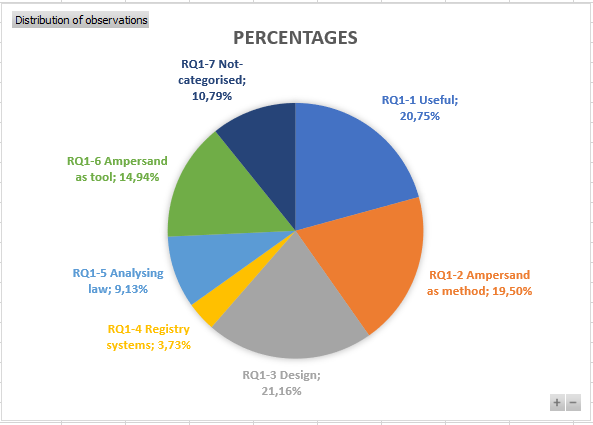
\includegraphics[width=0.7\textwidth]{docs/AF-SE/00_common/04_images/content_analysis.PNG}
    \caption{Content observations Distribution}
    \label{fig:content distribution}
\end{figure}

\def\head{\textbf{RQ1-1, Category:Useful, Reference to observation/interview}}
\begin{xltabular}{\textwidth}{|X|}
\caption{List of observations \head} \\ \hline 
\multicolumn{1}{|l|}{\head}  \\ \hline 
\endfirsthead
{{\bfseries \tablename\ \thetable{} -- continued from previous page}} \\
\hline 
\multicolumn{1}{|l|}{\head}  \\ \hline 
\endhead
\hline \multicolumn{1}{|r|}{{Continued on next page}} \\ \hline
\endfoot \hline \hline
\endlastfoot

\PCIS{int:I-4.5}\\
\PCOS{obs:rq1-11}\\
\PCOS{obs:rq1-18}\\
\PCOS{obs:rq1-13:17-10}\\
\PCOS{obs:rq1-36:29-9}\\
\PCOS{obs:rq1-47:27-10}\\
\PCOS{obs:rq1-6:21-10}\\
\PCOS{obs:rq4-8:22-11}\\

\PCOS{obs:rq1-17}\\
\PCOS{obs:rq1-60:9-11}\\
\PCOS{obs:rq1-96:30-12}\\

\PCIS{int:I-3.7}\\
\PCOS{obs:rq1-2}\\
\PCOS{obs:rq1-25:12-9}\\
\PCOS{obs:rq1-31:14-9}\\

\PCOS{obs:rq1-42:19-10}\\
\PCOS{obs:rq1-45:24-10}\\
\PCOS{obs:rq1-46:24-10}\\
\PCOS{obs:rq1-97:30-12}\\

\PCIS{int:I-3.2}\\
\PCOS{obs:rq3-7}\\

\PCOS{obs:rq1-42:21-10}\\

\PCIS{int:I-1.3}\\
\PCIS{int:I-1.8}\\
\PCIS{int:I-2.10}\\
\PCOS{obs:rq1-62:10-11}\\

\PCIS{int:I-2.2}\\
\PCOS{obs:rq4-2}\\
\PCOS{obs:rq4-5}\\
\PCOS{obs:rq1-70:14-11}\\
\PCOS{obs:rq1-72:14-11}\\
\PCOS{obs:rq1-73:14-11}\\
\PCOS{obs:rq1-74:16-11}\\
\PCOS{obs:rq1-8:14-11}\\

\PCIS{int:I-2.5}\\
\PCIS{int:I-4.8}\\
\PCOS{obs:rq4-7}\\
\PCOS{obs:rq1-63:10-11}\\

\PCIS{int:I-4.6}\\
\PCOS{obs:rq2-18:16-11}\\

\PCIS{int:I-1.2}\\
\PCIS{int:I-1.6}\\

\PCIS{int:I-4.11}\\
\PCIS{int:I-4.12}\\
\PCIS{int:I-4.3}\\
\PCIS{int:I-4.9}\\
\PCOS{obs:rq1-39:3-10}\\
\PCOS{obs:rq1-7:10-11}\\
\PCOS{obs:rq2-16:19-10}\\
\PCOS{obs:rq3-16:24-10}\\


%-	rq1-11 Implementation in Docker with RAP creates new directories all the time.
%\\-	rq1-13:17-10: The setup of Ampersand in local environment is specific and not self-explanatory.
%\\-	rq1-17 Applying a rule requires a lot of patience and practice.
%\\-	rq1-18 Can not find an example on the internet, only in the repo of Ampersand itself.
%\\-	rq1-39:3-10: Do not forget to create delete rules in addition to append and edit rules in the {rule}\textbf{s} in the context of the \A{Lifecycle} approach.
%\\-	rq1-42:19-10: Immediately add the description when recording a {concept} and \A{relation}.
%\\-	rq1-42:21-10: It is easy to deviate from the legal texts.
%\\-	rq1-45:24-10: Overview within a Ampersandscript is difficult to maintain and obtain.
%\\-	rq1-46:24-10: There is no find able relationship between the \A{relation} and the {concept} in the script.
%\\-	rq1-47:27-10: Detecting a bug.
%\-	rq1-60:9-11: The process of writing a \A{Ampersand} script is not without practice.
%\-	rq1-62:10-11: There has be the \A{architecture} link between the {law core} and the {register core}
%\-	rq1-63:10-11: Ampersand is \A{flexible} by extension concepts and relationships.
%\\-	rq1-7:10-11: Each \A{relation} is part of a record structure.
%\\-	rq1-70:14-11: Postman works with api/v1/resource, e.g. GET \url{localhost/api/v1/resource/Person/P001/Person}, retrieves that of an existing person.
%\\-	rq1-73:14-11: Ampersand can be used from other applications through \A{api}'s, but the return values are next to the requested information also messages and not message codes.
%\\-	rq1-96:30-12: Skill in scripting within \A{Ampersand} is quickly lost if you don't do this frequently.
%\\-	rq1-97:30-12: By puzzling with Ampersand people quickly forget to make correct \A{documentation}.
%\\-	rq2-12:19-10: TOT has the property that this must be entered in the \A{interface} because otherwise the data will not be saved.
%\\-	rq2-16:19-10/11-11: Ampersand has a hard time determining a period.
%\\-	rq2-18:16-11: Good to realize that the {meaning} you write down also ends up in the \A{Conceptual analysis}.
%\\-	rq3-7 Adding \A{documentation} with the correct description to a concept and relation is not so easy.
%\\-	rq4-5 Postman used for \A{api} link with Ampersand.
%\\-	rq4-7 What happens if \A{Ampersand} is implemented and there are changes in the structure (normal for software)
%\\-	rq4-8:22-11: The team behind \A{Ampersand} is very dedicated.
%\\-	 rq1-8:14-11: No swagger is created for the \A{api}
%\\-	rq1-46:24-10: There is no find able relationship between the {relation} and the \A{concept} in the script.
%\\-	 rq1-6:21-10/30-10: \A{Docker} is also another thing to learn.
%\\-	 rq1-17 Applying a \A{rule}\textbf{s} takes a lot of patience and practice.
%\\-	 rq2-4:30-9: Which agreements must be made regarding the structure of the descriptions for \A{Conceptual analysis}.
%\\-	 rq3-16:24-10: For the Netherlands, we have a country table from the RvIG.
%\\-	 rq4-2 The \A{api} link works fine, but entire messages return.
%\\-	Ampersand can be interesting, because it will be able to clear conflicting matters from the law.
%\\-	The registry core, an architecture model of CIBG, uses shared concepts
%\\-	In addition, the implementation must be such that the effective dates of the specific amendments to the law are also taken into account.
%\\-	Ampersand's possible positioning is to use it as an interpreter of legislation and regulations
%\\-	Ampersand has APIs and that is interesting to be able to link with
%\\-	When maintenance takes place on the model, how do we get from one model to another
%\\-	Ampersand's approach is in line with the \acrlong{rk}, but not at the implementation level.
%\\-	An addition of Ampersand is that a prototype is made that can also be tested. 
%\\-	A draft of the conceptual analysis is available and this is experienced as trusted by the lawyer. 
%\\-	Going through the law should be a first step for the conceptual analysis.
%\\-	The prototype shown is not easy for the user to understand.
%\\-	Ampersand's deployment could be applied to new tasks.
%\\-	For use, the question is how quickly a base is set up
%\\-	Ampersand method is a way of writing things down
%\\-	How is the maintenance of the system? A new model is always made with the help of Ampersand.
%\\-	The learning curve doesn't seem that big. 
%\\-	The question is whether the system will only work for simple registers or whether we can also use it to tackle complex registers.
%\\-	A follow-up study could be to make a comparison between a system built traditionally and a system built on the Ampersand method. 

\end{xltabular}


\def\head{\textbf{RQ1-2, Category:Ampersand as method, Reference to observation/interview}}
\begin{xltabular}{\textwidth}{|X|}
\caption{List of observations \head} \\ \hline 
\multicolumn{1}{|l|}{\head}  \\ \hline 
\endfirsthead
{{\bfseries \tablename\ \thetable{} -- continued from previous page}} \\
\hline 
\multicolumn{1}{|l|}{\head}  \\ \hline 
\endhead
\hline \multicolumn{1}{|r|}{{Continued on next page}} \\ \hline
\endfoot \hline \hline
\endlastfoot
\PCOS{obs:rq1-30:12-9}\\
\PCOS{obs:rq1-33:14-9}\\
\PCOS{obs:rq1-38:3-10}\\
\PCOS{obs:rq1-46:24-10}\\
\PCOS{obs:rq1-80:20-11}\\
\PCOS{obs:rq2-4:30-9}\\
\PCOS{obs:rq1-3}\\
\PCOS{obs:rq2-2}\\
\PCOS{obs:rq1-21:7-11}\\
\PCOS{obs:rq1-58:8-11}\\
\PCOS{obs:rq2-11:19-10}\\
\PCOS{obs:rq2-12:19-10}\\
\PCOS{obs:rq2-13:19-10}\\
\PCOS{obs:rq2-5:2-10}\\
\PCOS{obs:rq1-4}\\
\PCOS{obs:rq1-61:9-11}\\
\PCOS{obs:rq1-63:10-11}\\
\PCOS{obs:rq1-67:11-11}\\
\PCOS{obs:rq2-19:16-11}\\
\PCOS{obs:rq2-6:2-10}\\
\PCOS{obs:rq1-79:20-11}\\
\PCOS{obs:rq1-91:14-12}\\
\PCIS{int:I-1.4}\\
\PCIS{int:I-3.7}\\
\PCIS{int:I-4.13}\\
\PCOS{obs:rq1-42:19-10}\\
\PCOS{obs:rq1-51:2-11}\\
\PCOS{obs:rq1-84:30-11}\\
\PCIS{int:I-1.8}\\
\PCIS{int:I-2.11}\\
\PCIS{int:I-3.1}\\
\PCIS{int:I-3.2}\\
\PCIS{int:I-4.2}\\
\PCOS{obs:rq1-57-1:7-11}\\
\PCIS{int:I-1.1}\\
\PCIS{int:I-1.9}\\
\PCIS{int:I-4.10}\\
\PCIS{int:I-4.14}\\
\PCIS{int:I-4.5}\\
\PCIS{int:I-4.9}\\
\PCOS{obs:rq1-55:2-11}\\
\PCOS{obs:rq1-7:10-11}\\
\PCOS{obs:rq2-10:19-10}\\
\PCOS{obs:rq2-14:19-10}\\
\PCOS{obs:rq2-8:7-10}\\

\end{xltabular}


\def\head{\textbf{RQ1-3, Category:Design, Reference to observation/interview}}
\begin{xltabular}{\textwidth}{|X|}
\caption{List of observations \head} \\ \hline 
\multicolumn{1}{|l|}{\head}  \\ \hline 
\endfirsthead
{{\bfseries \tablename\ \thetable{} -- continued from previous page}} \\
\hline 
\multicolumn{1}{|l|}{\head}  \\ \hline 
\endhead
\hline \multicolumn{1}{|r|}{{Continued on next page}} \\ \hline
\endfoot \hline \hline
\endlastfoot
\PCIS{int:I-1.12}\\
\PCIS{int:I-1.3}\\
\PCIS{int:I-2.1}\\
\PCIS{int:I-2.6}\\
\PCIS{int:I-2.7}\\
\PCIS{int:I-2.8}\\
\PCOS{obs:rq4-1}\\
\PCOS{obs:rq4-3}\\
\PCOS{obs:rq1-63:10-11}\\
\PCOS{obs:rq1-89:7-12}\\

\PCOS{obs:rq1-1}\\
\PCOS{obs:rq1-75:20-11}\\
\PCOS{obs:rq1-78:20-11}\\
\PCOS{obs:rq1-99:6-1}\\
\PCOS{obs:rq2-18:16-11}\\

\PCOS{obs:rq1-39:3-10}\\
\PCOS{obs:rq1-95:29-12}\\

\PCOS{obs:rq1-92:14-12}\\
\PCOS{obs:rq1-93:19-12}\\
\PCOS{obs:rq3-8:19-9}\\

\PCIS{int:I-4.2}\\
\PCOS{obs:rq1-36:3-10}\\
\PCOS{obs:rq1-69:14-11}\\

\PCIS{int:I-4.7}\\
\PCOS{obs:rq2-17:10-11}\\
\PCOS{obs:rq3-10:12-10}\\
\PCOS{obs:rq3-11:12-10}\\

\PCOS{obs:rq1-71:14-11}\\

\PCIS{int:I-1.10}\\
\PCIS{int:I-3.4}\\
\PCIS{int:I-3.5}\\
\PCIS{int:I-4.8}\\

\PCIS{int:I-4.4}\\
\PCOS{obs:rq4-2}\\
\PCOS{obs:rq4-4}\\
\PCOS{obs:rq4-7}\\
\PCOS{obs:rq2-14:19-10}\\
\PCOS{obs:rq2-15:19-10}\\
\PCOS{obs:rq2-9:7-10}\\


\end{xltabular}

\def\head{\textbf{RQ1-4, Category:Registry systems, Reference to observation/interview}}
\begin{xltabular}{\textwidth}{|X|}
\caption{List of observations \head} \\ \hline 
\multicolumn{1}{|l|}{\head}  \\ \hline 
\endfirsthead
{{\bfseries \tablename\ \thetable{} -- continued from previous page}} \\
\hline 
\multicolumn{1}{|l|}{\head}  \\ \hline 
\endhead
\hline \multicolumn{1}{|r|}{{Continued on next page}} \\ \hline
\endfoot \hline \hline
\endlastfoot
\PCIS{int:I-2.10}\\
\PCIS{int:I-2.6}\\
\PCIS{int:I-2.7}\\
\PCIS{int:I-2.9}\\

\PCOS{obs:rq1-85:30-11}\\
\PCOS{obs:rq1-92:14-12}\\
\PCOS{obs:rq3-8:19-9}\\
\PCOS{obs:rq3-9:19-9}\\
\end{xltabular}

\def\head{\textbf{RQ1-5, Category:Analysing law, Reference to observation/interview}}
\begin{xltabular}{\textwidth}{|X|}
\caption{List of observations \head} \\ \hline 
\multicolumn{1}{|l|}{\head}  \\ \hline 
\endfirsthead
{{\bfseries \tablename\ \thetable{} -- continued from previous page}} \\
\hline 
\multicolumn{1}{|l|}{\head}  \\ \hline 
\endhead
\hline \multicolumn{1}{|r|}{{Continued on next page}} \\ \hline
\endfoot \hline \hline
\endlastfoot
\PCOS{obs:rq3-4:12-9}\\
\PCOS{obs:rq1-26:12-9}\\
\PCOS{obs:rq1-27:12-9}\\
\PCOS{obs:rq1-29:12-9}\\
\PCOS{obs:rq3-15:24-10}\\

\PCOS{obs:rq1-23:24-10}\\
\PCOS{obs:rq1-35:14-9}\\
\PCOS{obs:rq1-41:19-10}\\
\PCOS{obs:rq1-42:21-10}\\

\PCOS{obs:rq2-1}\\
\PCOS{obs:rq3-2}\\

\PCOS{obs:rq1-24:12-9}\\
\PCOS{obs:rq1-25:12-9}\\
\PCOS{obs:rq1-31:14-9}\\

\PCIS{int:I-1.11}\\
\PCIS{int:I-1.8}\\
\PCIS{int:I-3.3}\\
\PCIS{int:I-3.6}\\
\PCIS{int:I-4.1}\\

\PCOS{obs:rq1-93:19-12}\\
\PCOS{obs:rq1-95:29-12}\\
\PCOS{obs:rq3-13:17-10}\\

\end{xltabular}


\def\head{\textbf{RQ1-6, Category:Ampersand as tool, Reference to observation/interview}}
\begin{xltabular}{\textwidth}{|X|}
\caption{List of observations \head} \\ \hline 
\multicolumn{1}{|l|}{\head}  \\ \hline 
\endfirsthead
{{\bfseries \tablename\ \thetable{} -- continued from previous page}} \\
\hline 
\multicolumn{1}{|l|}{\head}  \\ \hline 
\endhead
\hline \multicolumn{1}{|r|}{{Continued on next page}} \\ \hline
\endfoot \hline \hline
\endlastfoot
\PCOS{obs:rq1-15:4-10}\\
\PCOS{obs:rq1-81:20-11}\\
\PCOS{obs:rq1-82:20-11}\\
\PCOS{obs:rq1-90:14-12}\\
\PCOS{obs:rq1-22}\\
\PCOS{obs:rq1-49:30-10}\\
\PCOS{obs:rq1-63:10-11}\\
\PCOS{obs:rq1-85:30-11}\\
\PCOS{obs:rq1-89:7-12}\\
\PCOS{obs:rq1-92:14-12}\\

\PCOS{obs:rq1-12}\\
\PCOS{obs:rq1-50:30-10}\\
\PCOS{obs:rq4-4}\\
\PCOS{obs:rq1-40:10-10}\\
\PCOS{obs:rq1-53:2-11}\\
\PCOS{obs:rq1-83:27-11}\\

\PCOS{obs:rq1-9}\\
\PCOS{obs:rq1-48:27-10}\\
\PCOS{obs:rq2-16:19-10}\\

\PCIS{int:I-1.5}\\
\PCIS{int:I-1.7}\\
\PCIS{int:I-2.4}\\
\PCIS{int:I-2.5}\\
\PCOS{obs:rq4-7}\\

\PCIS{int:I-4.4}\\
\PCOS{obs:rq1-10}\\
\PCOS{obs:rq1-65:10-11}\\
\PCOS{obs:rq1-66:10-11}\\
\PCOS{obs:rq1-91:14-12}\\
\PCOS{obs:rq1-98:30-12}\\
\PCOS{obs:rq2-9:7-10}\\


\end{xltabular}

\def\head{\textbf{RQ1-7, Category:Not-categorised, Reference to observation/interview}}
\begin{xltabular}{\textwidth}{|X|}
\caption{List of observations \head} \\ \hline 
\multicolumn{1}{|l|}{\head}  \\ \hline 
\endfirsthead
{{\bfseries \tablename\ \thetable{} -- continued from previous page}} \\
\hline 
\multicolumn{1}{|l|}{\head}  \\ \hline 
\endhead
\hline \multicolumn{1}{|r|}{{Continued on next page}} \\ \hline
\endfoot \hline \hline
\endlastfoot
\PCIS{int:I-2.3}\\
\PCIS{int:I-3.7}\\
\PCOS{obs:rq1-11}\\
\PCOS{obs:rq1-16}\\
\PCOS{obs:rq3-3:12-9}\\
\PCOS{obs:rq1-32:14-9}\\
\PCOS{obs:rq1-33:9-1}\\
\PCOS{obs:rq1-34:14-9}\\
\PCOS{obs:rq1-43:23-10}\\
\PCOS{obs:rq1-44:23-10}\\
\PCOS{obs:rq1-5:30-10}\\
\PCOS{obs:rq1-54:2-11}\\
\PCOS{obs:rq1-57-2:7-11}\\
\PCOS{obs:rq1-76:20-11}\\
\PCOS{obs:rq1-86:30-11}\\
\PCOS{obs:rq1-88:5-12}\\
\PCOS{obs:rq2-7:4-10}\\
\PCOS{obs:rq3-14:19-10}\\

\end{xltabular}

\newpage
\section{List of Functional Requirements}\label{appendix-functiontal-requirements}
\printindex[fr]

\newpage
\section{Adl scripts}\label{appendixAdl}
\lstinputlisting[caption=Persoon, label=lst:persoon]{../../big/0_generiek/Persoon.adl}
\newpage
\lstinputlisting[caption=PersoonInterface, label=lst:persoon-interface]{../../big/0_generiek/PersoonI.adl}
\newpage
\lstinputlisting[caption=Inschrijving,label=lst:inschrijving]{../../big/0_generiek/Inschrijving.adl}
\newpage
\lstinputlisting[caption=Register,label=lst:register]{../../big/0_generiek/Register.adl}
\newpage
\lstinputlisting[caption=Registratie,label=lst:registratie]{../../big/0_generiek/Registratie.adl}
\newpage
\lstinputlisting[caption=ArtsRegister, label=lst:arts-register]{../../big/1_artsRegister/Main.adl}


\newpage
\section{Prototype}\label{appendixPrototype}
\begin{figure}[ht]
    \centering
    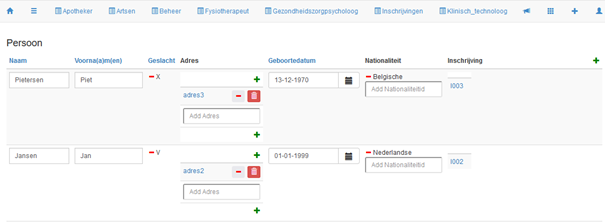
\includegraphics[width=\textwidth]{/prototype/personen.png}
    \caption{Personen}
    \label{fig:proto-personen}
\end{figure}

\begin{figure}[hb]
    \centering
    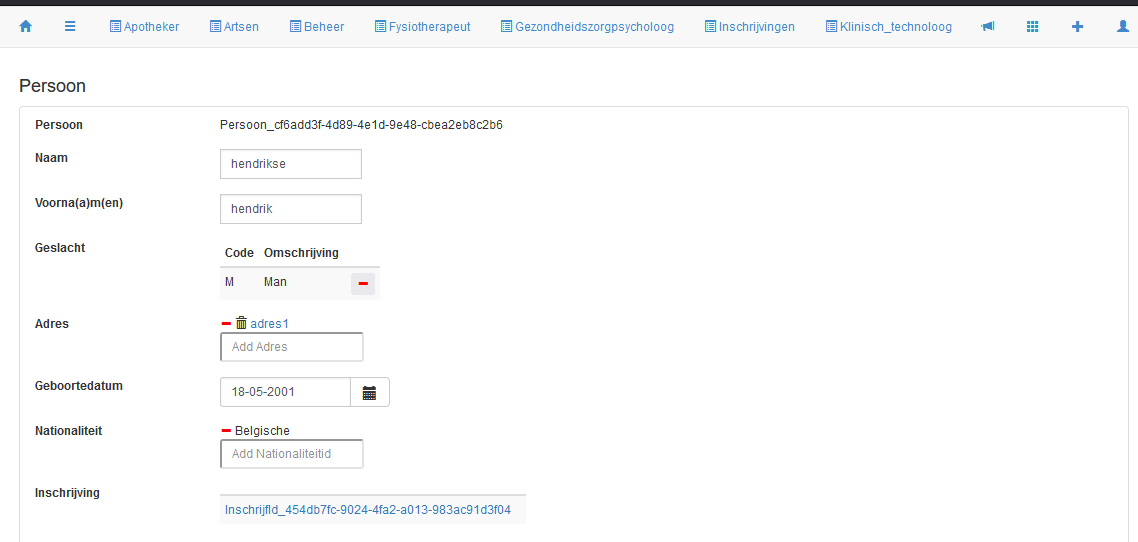
\includegraphics[width=\textwidth]{/prototype/persoon.png}
    \caption{Persoon}
    \label{fig:proto-persoon}
\end{figure}

\newpage

\begin{figure}[ht]
    \centering
    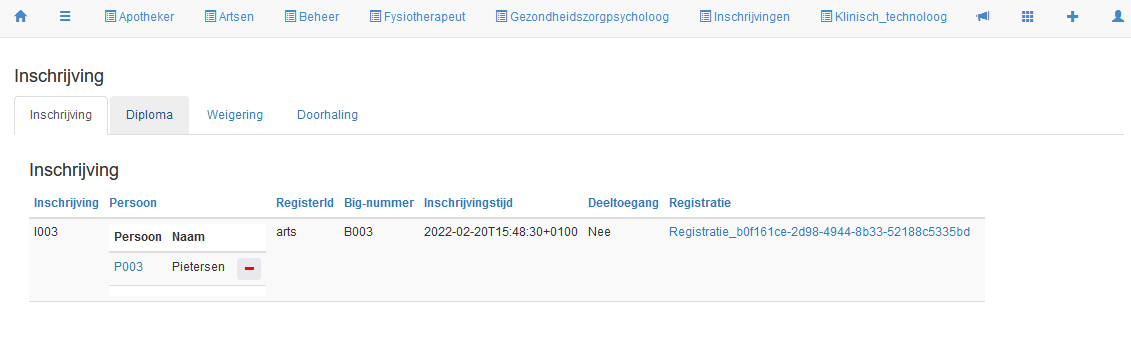
\includegraphics[width=\textwidth]{/prototype/inschrijving.PNG}
    \caption{Inschrijving}
    \label{fig:proto-inschrijving}
\end{figure}

\begin{figure}[!hb]
    \centering
    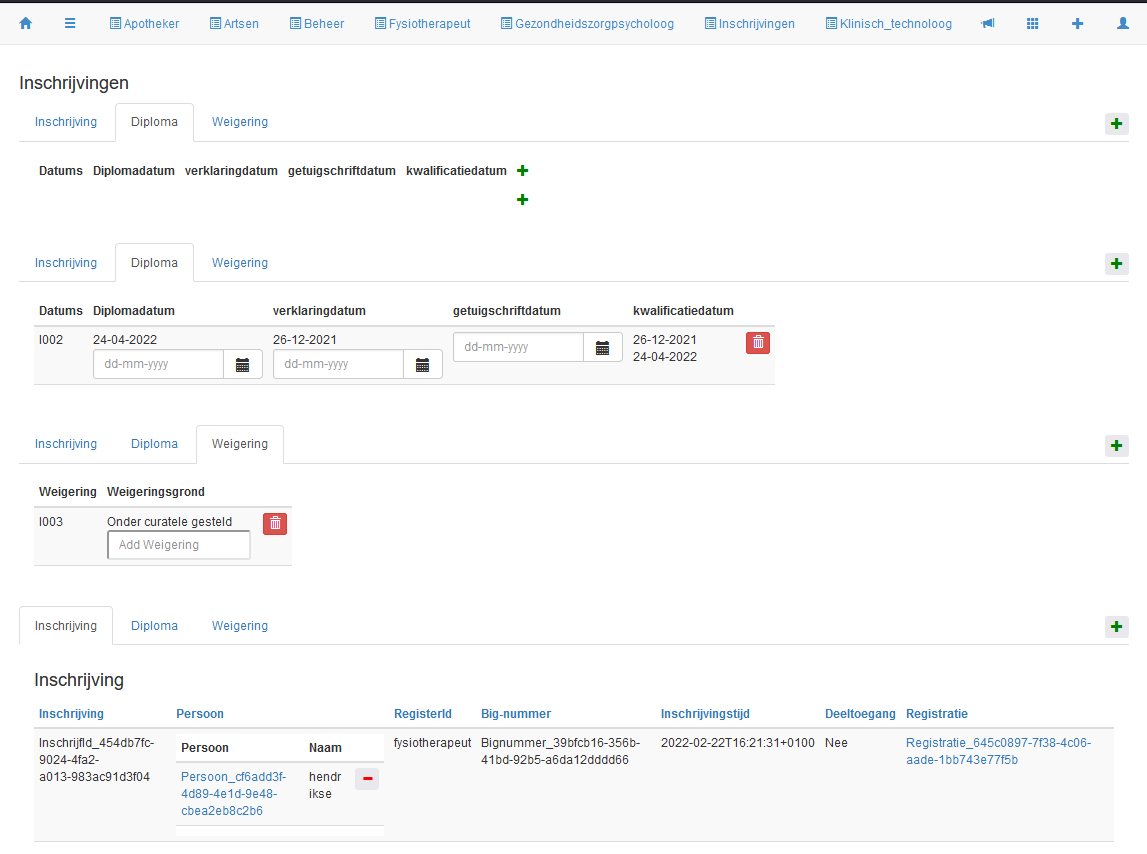
\includegraphics[width=\textwidth]{/prototype/inschrijvingdiplomaenweigergrond.PNG}
    \caption{Inschrijving-diploma-en-weigergrond}
    \label{fig:proto-inschrijving-diploma-en-weigergrond}
\end{figure}

\newpage

\begin{figure}[ht]
    \centering
    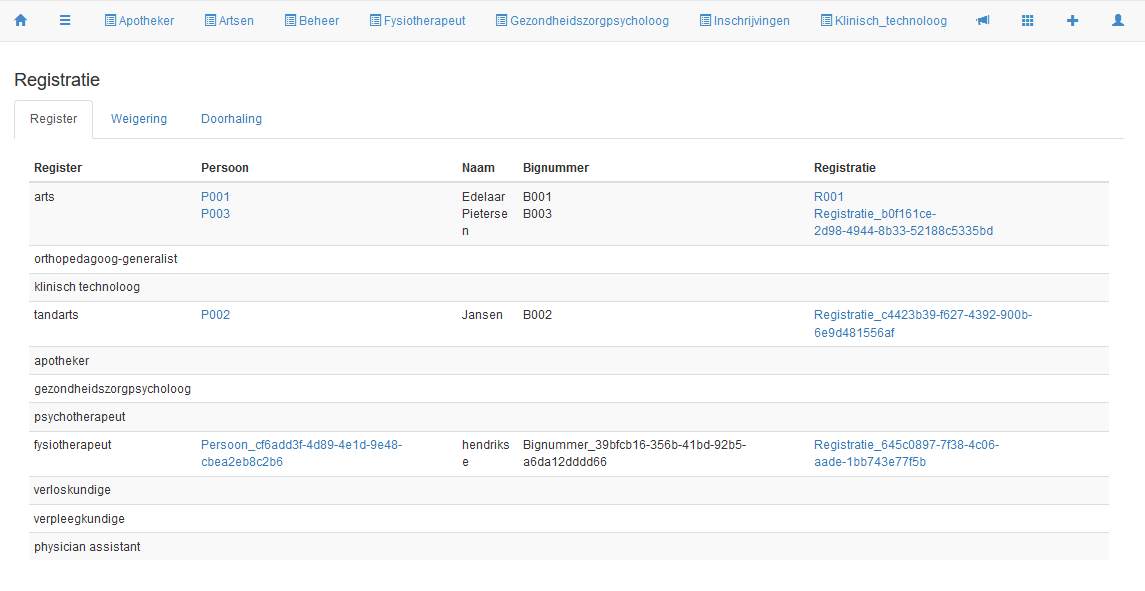
\includegraphics[width=\textwidth]{/prototype/registratie.PNG}
    \caption{Registratie}
    \label{fig:proto-registratie}
\end{figure}

\begin{figure}[!hb]
    \centering
    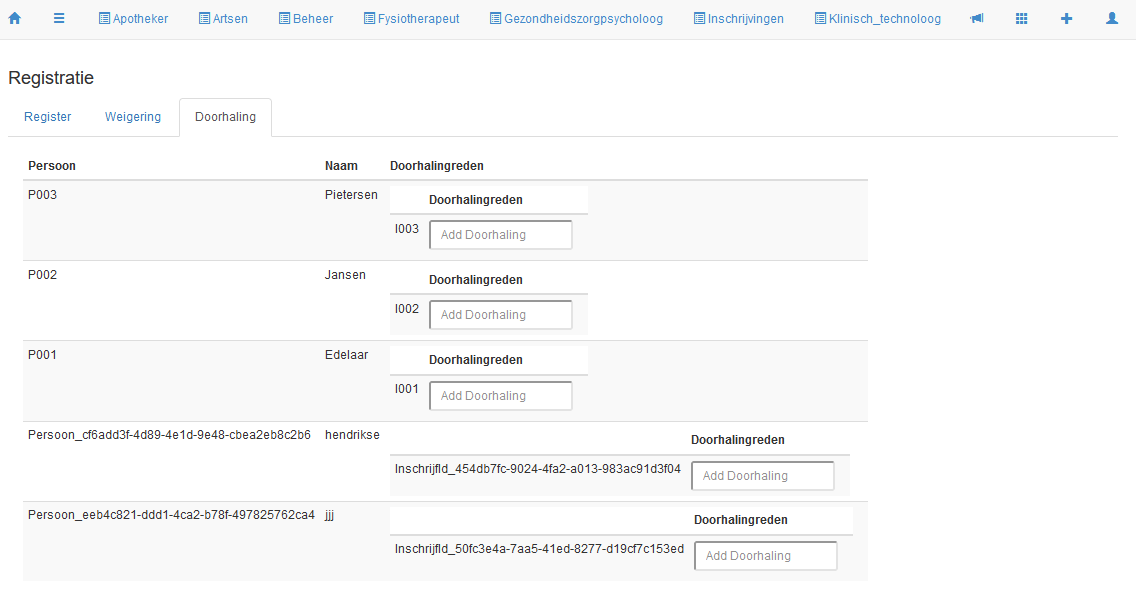
\includegraphics[width=\textwidth]{/prototype/registratiedoorhaling.PNG}
    \caption{Registratie doorhaling}
    \label{fig:proto-registratie-doorhaling}
\end{figure}
\newpage
\begin{figure}[ht]
    \centering
    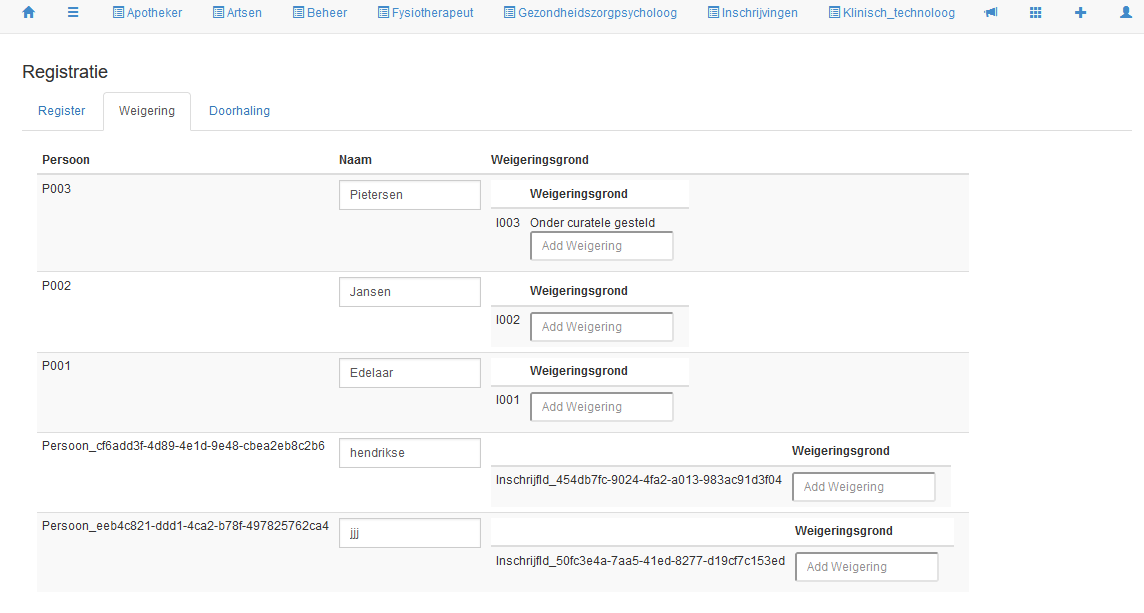
\includegraphics[width=\textwidth]{/prototype/registratieweigering.PNG}
    \caption{Registratie weigering}
    \label{fig:proto-registratie-weigering}
\end{figure}

\begin{figure}[!hb]
    \centering
    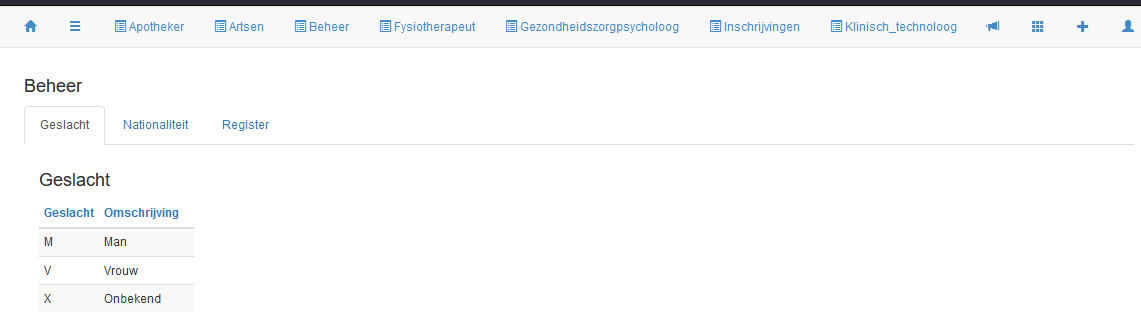
\includegraphics[width=\textwidth]{/prototype/beheergeslacht.PNG}
    \caption{Beheergeslacht}
    \label{fig:proto-beheergeslacht}
\end{figure}
\newpage
\begin{figure}[ht]
    \centering
    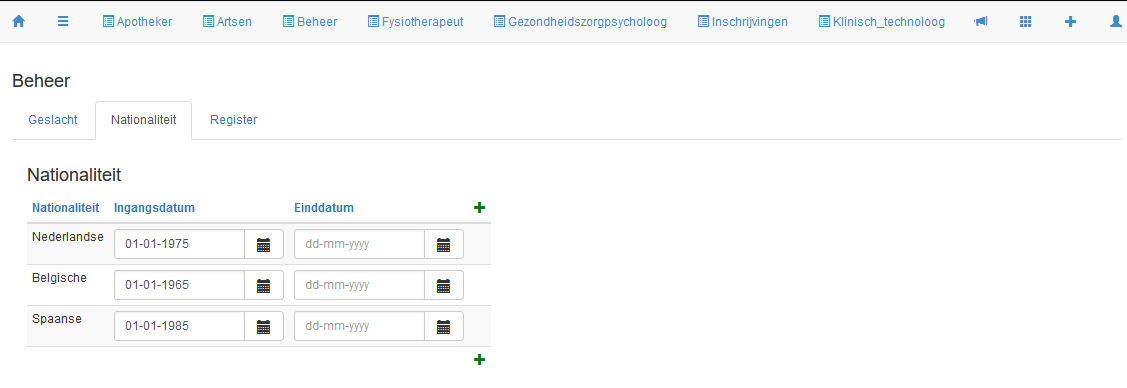
\includegraphics[width=\textwidth]{/prototype/beheernationaliteit.PNG}
    \caption{Beheernationaliteit}
    \label{fig:proto-beheernationaliteit}
\end{figure}

\begin{figure}[!hb]
    \centering
    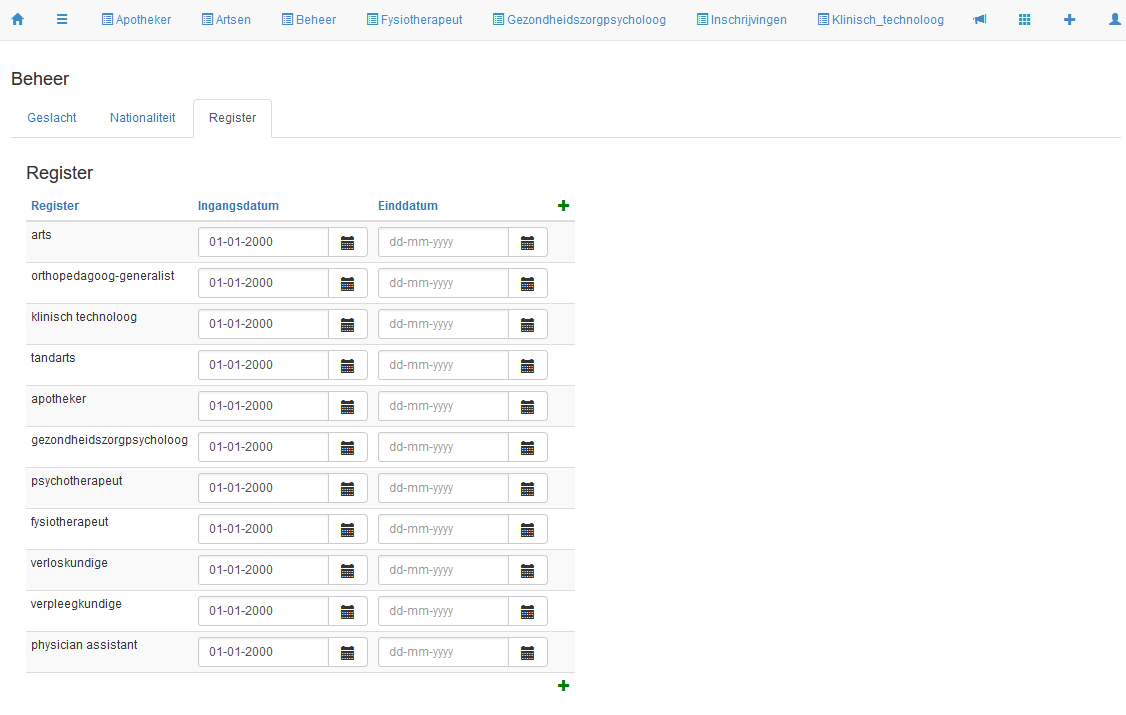
\includegraphics[width=\textwidth]{/prototype/beheerregister.PNG}
    \caption{Beheerregister}
    \label{fig:proto-beheerregister}
\end{figure}
\newpage
\begin{figure}[ht]
    \centering
    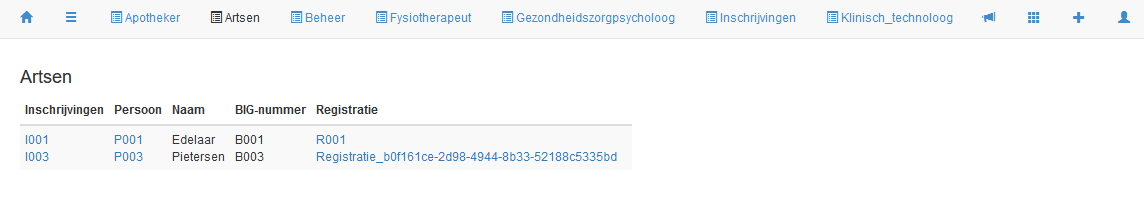
\includegraphics[width=\textwidth]{/prototype/artsregister.PNG}
    \caption{Artsregister}
    \label{fig:proto-artsregister}
\end{figure}

\newpage
\section{Technical Datamodel}\label{appendixTechDatamodel}
\begin{figure}[!htp]
    \centering
        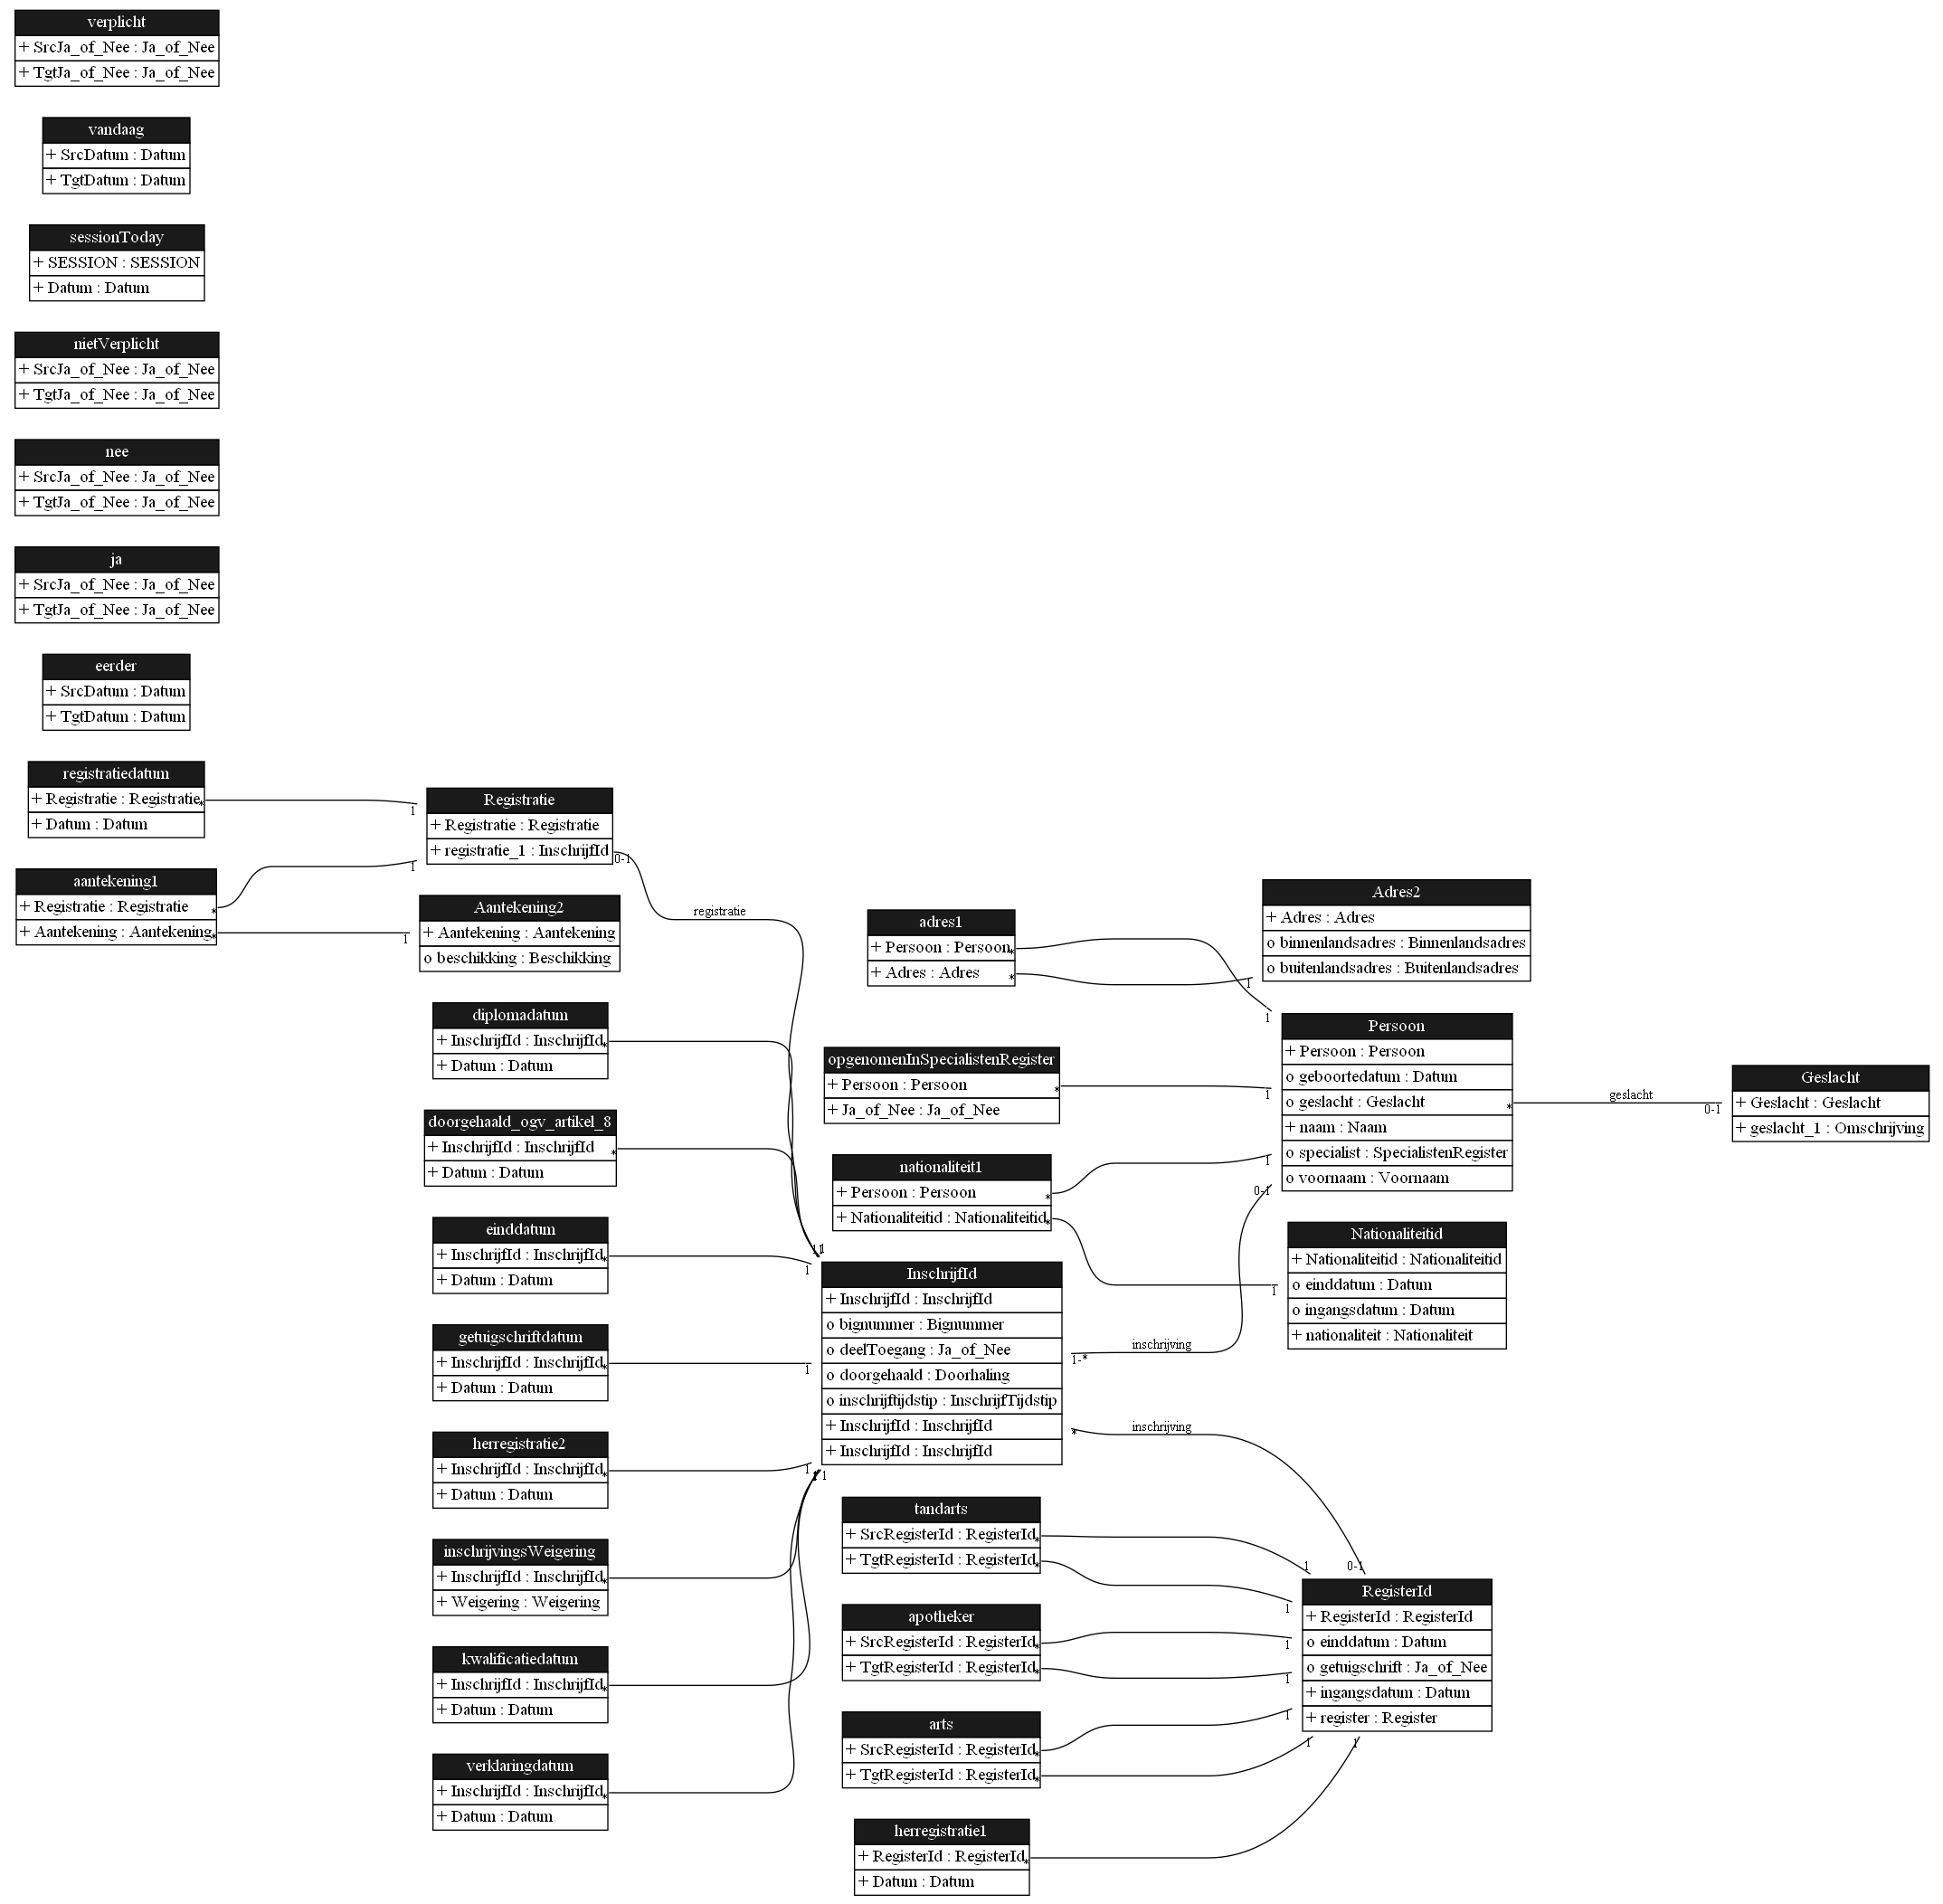
\includegraphics[width=0.8\textwidth]
            {../images/TechnicalDataModel.png}
        \caption{TechnicalDataModel}
    \label{fig:TechnicalDataModel}
\end{figure}



\newpage
\section{Conceptual analysis}\label{ConceptualAnalysis}
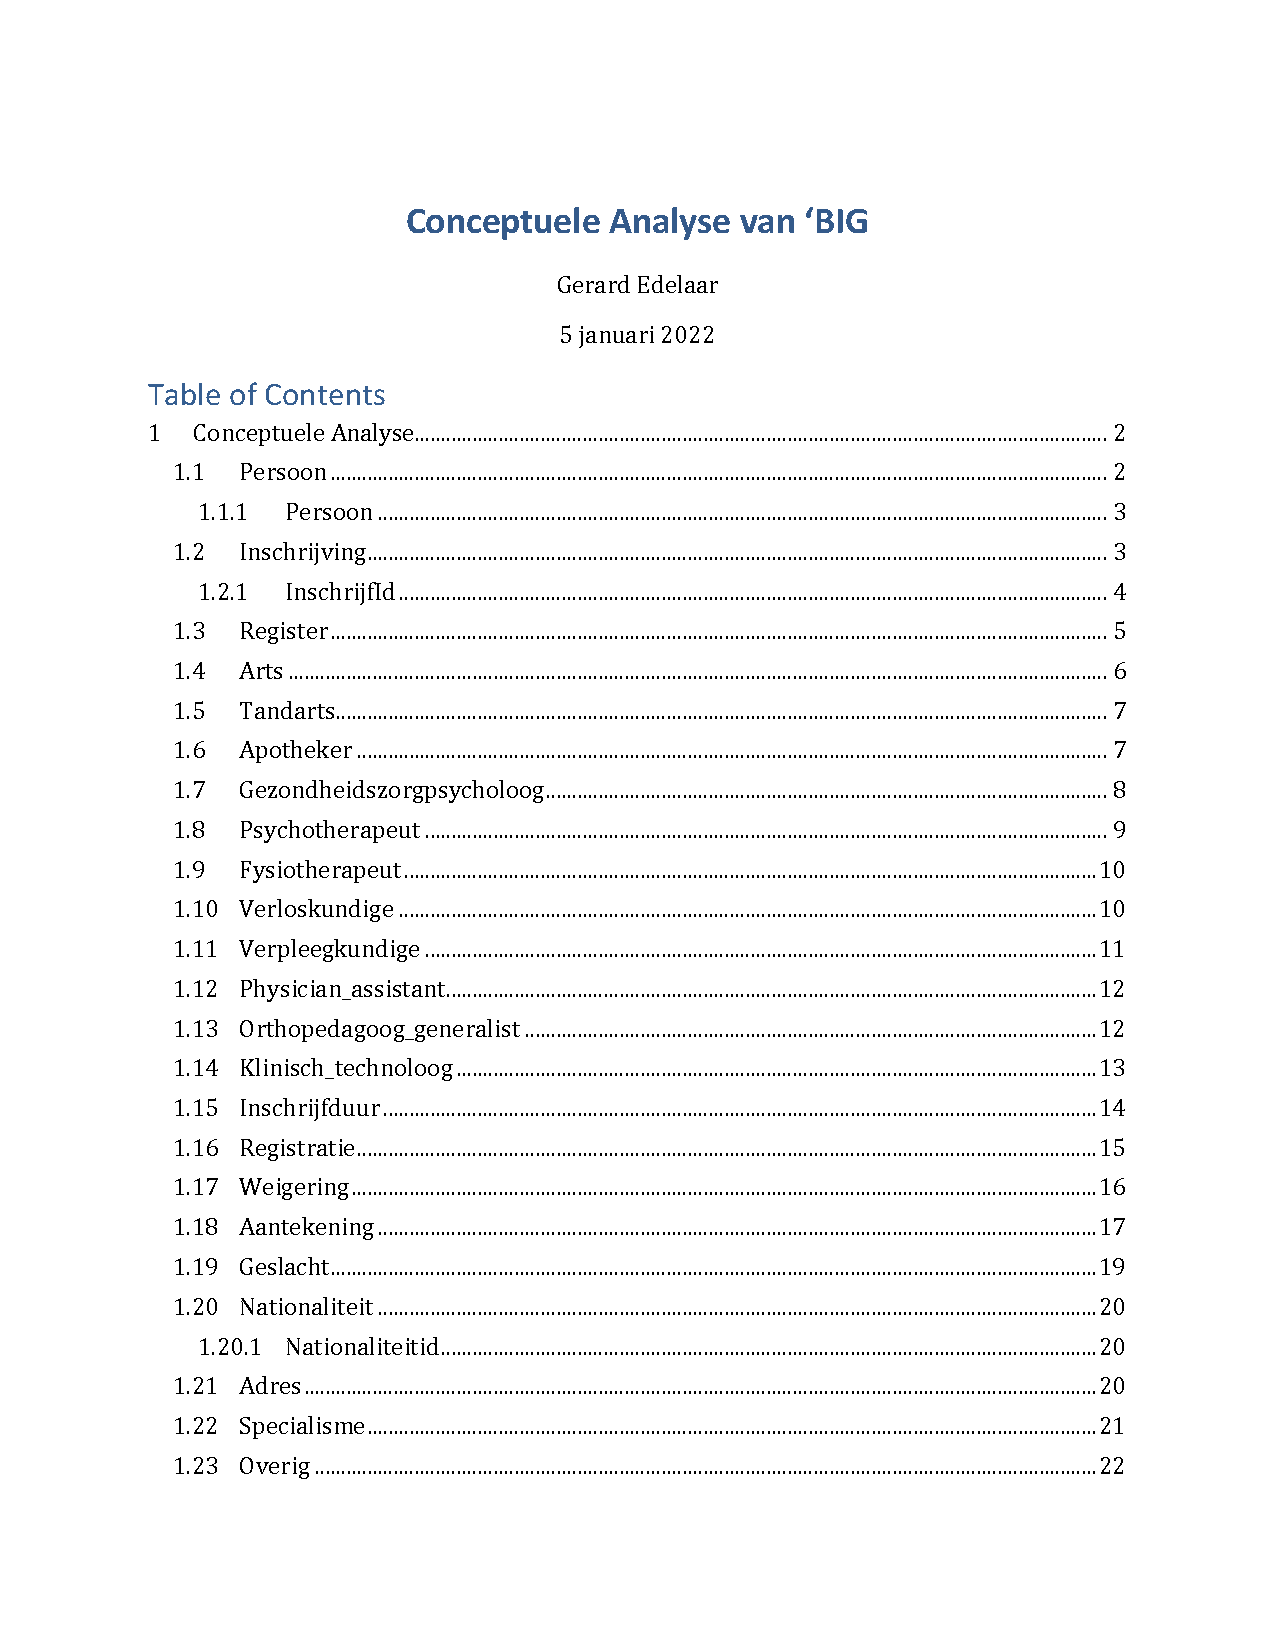
\includepdf[pages=-]{../ConceptualAnalysis/wetbig.pdf}



\includepdf[pages=-]{myfile.pdf}
\end{document}




